\documentclass{beamer}
\usetheme{Berlin}

\usepackage[T1]{fontenc}
\usepackage{textcomp}
\usepackage[utf8x]{inputenc}
\usepackage[ngerman]{babel}

\usepackage{amsmath, amsfonts, amsthm, mathtools, amssymb}

\usepackage{pgfplots}
\pgfplotsset{compat=1.16}


\renewcommand{\Im}{\operatorname{Im}}
\renewcommand{\Re}{\operatorname{Re}}

\newcommand{\N}{\mathbb{N}}
\newcommand{\Q}{\mathbb{Q}}
\newcommand{\R}{\mathbb{R}}
\newcommand{\Z}{\mathbb{Z}}
\newcommand{\C}{\mathbb{C}}

\newcommand{\intd}{\mathrm{d}}
\newtheorem*{hypothesis}{Vermutung}
\newtheorem*{behauptung}{Behauptung}

\title{Die Riemannsche Zeta-Funktion}
\author{Josua Kugler}
\date{03.11.2020}

\begin{document}
%\includeonlyframes{current}
\titlepage
\section{Definition}
\begin{frame}%texorpdfstring{$\zeta$}{\unichar{"03B6}}
    \begin{definition}[Riemannsche $\zeta$-Funktion]
        \[
            \zeta(s) = \sum_{n = 1}^{\infty} \frac{1}{n^s}
        \]
    \end{definition}
\end{frame}
\begin{frame}
    \begin{lemma}[Konvergenzgebiet]
        $\zeta(s)$ konvergiert normal auf der offenen Halbebene $\Re s > 1$.
    \end{lemma}
    \begin{proof}
    \[\sum_{n=1}^\infty \left|\frac{1}{n^s}\right| =  \sum_{n=1}^\infty \left|\frac{1}{e^{\log(n)\cdot \Re s}}\right| \cdot \left|\frac{1}{e^{i \cdot \log(n) \cdot \Im s}}\right| = \sum_{n=1}^\infty \frac{1}{n^{\Re s}}.\] 
    %Diese Reihe konvergiert, wie aus der reellen Analysis bekannt, für $\Re s > 1$.
    \end{proof}

\end{frame}
\section{Eulerprodukt}
\begin{frame}
    \begin{lemma}[Eulerprodukt]
        Die Riemannsche $\zeta$-Funktion lässt sich als absolut konvergentes unendliches Produkt schreiben:
    \[
        \zeta(s) = \prod_{k\in \mathbb{N}}\frac{1}{1-p_k^{-s}}.
    \]
    Insbesondere gilt also $\zeta(s) \neq 0$ für $\Re s > 1$.
    \end{lemma}
\end{frame}
\begin{frame}[t]
    \begin{proof}
    \begin{align*}%geometrische Reihe
        \visible<5->{\lim\limits_{m \to \infty}}\visible<2->{\prod_{k=1}^m} \frac{1}{1-p_k^{-s}} &= \only<5->{\lim\limits_{m \to \infty}}\only<2->{\prod_{k=1}^m} \sum_{\nu = 0}^\infty \frac{1}{p_k^{\nu s}}\\
        %Cauchyscher Multiplikationssatz
        \visible<3->{&=} \only<5->{\lim\limits_{m \to \infty}} \visible<3->{\sum_{\nu_1,\dots, \nu_m = 0}^\infty (p_1^{\nu_1}\cdots p_m^{\nu_m})^{-s}}\visible<3->{\\}
        %Eindeutigkeit der Primfaktorzerlegung
        \visible<4->{&=} \only<5->{\lim\limits_{m\to \infty}} \visible<4->{\sum_{n = p_1^{\nu_1}\cdots p_m^{\nu_m}}n^{-s}\\}
        \only<7>{\prod_{k=1}^\infty \frac{1}{1-p_k^{-s}} }\visible<6->{ &= \sum_{n=1}^\infty n^{-s}}\invisible<1->{justsomespaceforkeepingthe=}
    \end{align*}
    \end{proof}
\end{frame}
\begin{frame}
    \begin{proof}[Beweis. (Absolute Konvergenz)]
        \begin{align*}
        \sum_p \left|1 - \frac{1}{1-p^{-s}}\right| &= \sum_p \left|1 - \sum_{m=0}^\infty p^{-ms}\right|\\
        &\leq \sum_p \sum_{m=1}^\infty \left| p^{-ms}\right|\\
        &\leq \sum_{n=1}^\infty \left|n^{-s}\right|
        \end{align*}
    \end{proof}
\end{frame}
\section{Analytische Fortsetzung}
\begin{frame}
    \only<1>{
    \begin{figure}
        \centering
        %% This file was created by tikzplotlib v0.9.4.
\begin{tikzpicture}

\definecolor{color0}{rgb}{0.271305,0.019942,0.347269}
\definecolor{color1}{rgb}{0.274952,0.037752,0.364543}
\definecolor{color2}{rgb}{0.277941,0.056324,0.381191}
\definecolor{color3}{rgb}{0.280267,0.073417,0.397163}
\definecolor{color4}{rgb}{0.281924,0.089666,0.412415}
\definecolor{color5}{rgb}{0.28291,0.105393,0.426902}
\definecolor{color6}{rgb}{0.283229,0.120777,0.440584}
\definecolor{color7}{rgb}{0.282884,0.13592,0.453427}
\definecolor{color8}{rgb}{0.281887,0.150881,0.465405}
\definecolor{color9}{rgb}{0.280255,0.165693,0.476498}
\definecolor{color10}{rgb}{0.278012,0.180367,0.486697}
\definecolor{color11}{rgb}{0.275191,0.194905,0.496005}
\definecolor{color12}{rgb}{0.271828,0.209303,0.504434}
\definecolor{color13}{rgb}{0.267968,0.223549,0.512008}
\definecolor{color14}{rgb}{0.263663,0.237631,0.518762}
\definecolor{color15}{rgb}{0.258965,0.251537,0.524736}
\definecolor{color16}{rgb}{0.253935,0.265254,0.529983}
\definecolor{color17}{rgb}{0.248629,0.278775,0.534556}
\definecolor{color18}{rgb}{0.243113,0.292092,0.538516}
\definecolor{color19}{rgb}{0.237441,0.305202,0.541921}
\definecolor{color20}{rgb}{0.231674,0.318106,0.544834}
\definecolor{color21}{rgb}{0.225863,0.330805,0.547314}
\definecolor{color22}{rgb}{0.220057,0.343307,0.549413}
\definecolor{color23}{rgb}{0.214298,0.355619,0.551184}
\definecolor{color24}{rgb}{0.208623,0.367752,0.552675}
\definecolor{color25}{rgb}{0.203063,0.379716,0.553925}
\definecolor{color26}{rgb}{0.197636,0.391528,0.554969}
\definecolor{color27}{rgb}{0.192357,0.403199,0.555836}
\definecolor{color28}{rgb}{0.187231,0.414746,0.556547}
\definecolor{color29}{rgb}{0.182256,0.426184,0.55712}
\definecolor{color30}{rgb}{0.177423,0.437527,0.557565}
\definecolor{color31}{rgb}{0.172719,0.448791,0.557885}
\definecolor{color32}{rgb}{0.168126,0.459988,0.558082}
\definecolor{color33}{rgb}{0.163625,0.471133,0.558148}
\definecolor{color34}{rgb}{0.159194,0.482237,0.558073}
\definecolor{color35}{rgb}{0.154815,0.493313,0.55784}
\definecolor{color36}{rgb}{0.150476,0.504369,0.55743}
\definecolor{color37}{rgb}{0.14618,0.515413,0.556823}
\definecolor{color38}{rgb}{0.141935,0.526453,0.555991}
\definecolor{color39}{rgb}{0.13777,0.537492,0.554906}
\definecolor{color40}{rgb}{0.133743,0.548535,0.553541}
\definecolor{color41}{rgb}{0.129933,0.559582,0.551864}
\definecolor{color42}{rgb}{0.126453,0.570633,0.549841}
\definecolor{color43}{rgb}{0.123463,0.581687,0.547445}
\definecolor{color44}{rgb}{0.121148,0.592739,0.544641}
\definecolor{color45}{rgb}{0.119738,0.603785,0.5414}
\definecolor{color46}{rgb}{0.119483,0.614817,0.537692}
\definecolor{color47}{rgb}{0.120638,0.625828,0.533488}
\definecolor{color48}{rgb}{0.123444,0.636809,0.528763}
\definecolor{color49}{rgb}{0.128087,0.647749,0.523491}
\definecolor{color50}{rgb}{0.134692,0.658636,0.517649}
\definecolor{color51}{rgb}{0.143303,0.669459,0.511215}
\definecolor{color52}{rgb}{0.153894,0.680203,0.504172}
\definecolor{color53}{rgb}{0.166383,0.690856,0.496502}
\definecolor{color54}{rgb}{0.180653,0.701402,0.488189}
\definecolor{color55}{rgb}{0.196571,0.711827,0.479221}
\definecolor{color56}{rgb}{0.214,0.722114,0.469588}
\definecolor{color57}{rgb}{0.232815,0.732247,0.459277}
\definecolor{color58}{rgb}{0.252899,0.742211,0.448284}
\definecolor{color59}{rgb}{0.274149,0.751988,0.436601}
\definecolor{color60}{rgb}{0.296479,0.761561,0.424223}
\definecolor{color61}{rgb}{0.319809,0.770914,0.411152}
\definecolor{color62}{rgb}{0.344074,0.780029,0.397381}
\definecolor{color63}{rgb}{0.369214,0.788888,0.382914}
\definecolor{color64}{rgb}{0.395174,0.797475,0.367757}
\definecolor{color65}{rgb}{0.421908,0.805774,0.35191}
\definecolor{color66}{rgb}{0.449368,0.813768,0.335384}
\definecolor{color67}{rgb}{0.477504,0.821444,0.318195}
\definecolor{color68}{rgb}{0.506271,0.828786,0.300362}
\definecolor{color69}{rgb}{0.535621,0.835785,0.281908}
\definecolor{color70}{rgb}{0.565498,0.84243,0.262877}
\definecolor{color71}{rgb}{0.595839,0.848717,0.243329}
\definecolor{color72}{rgb}{0.626579,0.854645,0.223353}
\definecolor{color73}{rgb}{0.657642,0.860219,0.203082}
\definecolor{color74}{rgb}{0.688944,0.865448,0.182725}
\definecolor{color75}{rgb}{0.720391,0.87035,0.162603}
\definecolor{color76}{rgb}{0.751884,0.874951,0.143228}
\definecolor{color77}{rgb}{0.783315,0.879285,0.125405}
\definecolor{color78}{rgb}{0.814576,0.883393,0.110347}
\definecolor{color79}{rgb}{0.845561,0.887322,0.099702}
\definecolor{color80}{rgb}{0.876168,0.891125,0.09525}
\definecolor{color81}{rgb}{0.906311,0.894855,0.098125}
\definecolor{color82}{rgb}{0.935904,0.89857,0.108131}
\definecolor{color83}{rgb}{0.964894,0.902323,0.123941}

\begin{axis}[
tick align=outside,
tick pos=left,
x grid style={white!69.0196078431373!black},
xmin=1.06, xmax=20.96,
xtick style={color=black},
y grid style={white!69.0196078431373!black},
ymin=-9.95, ymax=9.95,
ytick style={color=black},
extra x ticks = {1.06},
extra x tick labels = {$1$},
xlabel= $\operatorname{Re} s$,
ylabel = $\operatorname{Im} s$,
]
\path [draw=color0, very thin]
(axis cs:1.06,-2.33084279544282)
--(axis cs:1.06596415598527,-2.35)
--(axis cs:1.09156672832119,-2.45)
--(axis cs:1.11247128820641,-2.55)
--(axis cs:1.1287315172552,-2.65)
--(axis cs:1.14035252592001,-2.75)
--(axis cs:1.14729352858579,-2.85)
--(axis cs:1.14946901803413,-2.95)
--(axis cs:1.1467485783386,-3.05)
--(axis cs:1.13895539013389,-3.15)
--(axis cs:1.12586340738216,-3.25)
--(axis cs:1.10719311233359,-3.35)
--(axis cs:1.08260567841278,-3.45)
--(axis cs:1.06,-3.52396190003257);

\path [draw=color0, very thin]
(axis cs:1.06,3.62396190003257)
--(axis cs:1.08260567841278,3.55)
--(axis cs:1.10719311233359,3.45)
--(axis cs:1.12586340738216,3.35)
--(axis cs:1.13895539013389,3.25)
--(axis cs:1.1467485783386,3.15)
--(axis cs:1.14946901803413,3.05)
--(axis cs:1.14729352858579,2.95)
--(axis cs:1.14035252592001,2.85)
--(axis cs:1.1287315172552,2.75)
--(axis cs:1.11247128820641,2.65)
--(axis cs:1.09156672832119,2.55)
--(axis cs:1.06596415598527,2.45)
--(axis cs:1.06,2.43084279544282);

\path [draw=color1, very thin]
(axis cs:1.06,-1.94512402462132)
--(axis cs:1.06277515639247,-1.95)
--(axis cs:1.11275425369982,-2.05)
--(axis cs:1.15751289048816,-2.15)
--(axis cs:1.16,-2.15640575993301)
--(axis cs:1.20010342523948,-2.25)
--(axis cs:1.23758308391499,-2.35)
--(axis cs:1.26,-2.4196079915338)
--(axis cs:1.27074760014764,-2.45)
--(axis cs:1.30019371371818,-2.55)
--(axis cs:1.32451914938554,-2.65)
--(axis cs:1.3438769042583,-2.75)
--(axis cs:1.35835007466792,-2.85)
--(axis cs:1.36,-2.86761611688574)
--(axis cs:1.36840981748404,-2.95)
--(axis cs:1.37335576093469,-3.05)
--(axis cs:1.37303307471321,-3.15)
--(axis cs:1.36732258058104,-3.25)
--(axis cs:1.36,-3.31571057185058)
--(axis cs:1.35622423758699,-3.35)
--(axis cs:1.33987876586398,-3.45)
--(axis cs:1.31761462777415,-3.55)
--(axis cs:1.28903635461633,-3.65)
--(axis cs:1.26,-3.73271384934331)
--(axis cs:1.2539079830586,-3.75)
--(axis cs:1.21274149672585,-3.85)
--(axis cs:1.16371280040037,-3.95)
--(axis cs:1.16,-3.95673740781451)
--(axis cs:1.10778316404305,-4.05)
--(axis cs:1.06,-4.12422617803139);

\path [draw=color1, very thin]
(axis cs:1.06,4.22422617803139)
--(axis cs:1.10778316404305,4.15)
--(axis cs:1.16,4.05673740781451)
--(axis cs:1.16371280040037,4.05)
--(axis cs:1.21274149672585,3.95)
--(axis cs:1.2539079830586,3.85)
--(axis cs:1.26,3.83271384934331)
--(axis cs:1.28903635461633,3.75)
--(axis cs:1.31761462777415,3.65)
--(axis cs:1.33987876586398,3.55)
--(axis cs:1.35622423758699,3.45)
--(axis cs:1.36,3.41571057185058)
--(axis cs:1.36732258058104,3.35)
--(axis cs:1.37303307471321,3.25)
--(axis cs:1.37335576093469,3.15)
--(axis cs:1.36840981748404,3.05)
--(axis cs:1.36,2.96761611688574)
--(axis cs:1.35835007466792,2.95)
--(axis cs:1.3438769042583,2.85)
--(axis cs:1.32451914938554,2.75)
--(axis cs:1.30019371371818,2.65)
--(axis cs:1.27074760014764,2.55)
--(axis cs:1.26,2.5196079915338)
--(axis cs:1.23758308391499,2.45)
--(axis cs:1.20010342523948,2.35)
--(axis cs:1.16,2.25640575993301)
--(axis cs:1.15751289048816,2.25)
--(axis cs:1.11275425369982,2.15)
--(axis cs:1.06277515639247,2.05)
--(axis cs:1.06,2.04512402462132);

\path [draw=color2, very thin]
(axis cs:1.06,-1.71169624804311)
--(axis cs:1.08779794432482,-1.75)
--(axis cs:1.15286996472351,-1.85)
--(axis cs:1.16,-1.86230457440359)
--(axis cs:1.21669914538333,-1.95)
--(axis cs:1.26,-2.02502809961443)
--(axis cs:1.27600753631156,-2.05)
--(axis cs:1.3324116741742,-2.15)
--(axis cs:1.36,-2.20548128784433)
--(axis cs:1.38441214831725,-2.25)
--(axis cs:1.43221355883815,-2.35)
--(axis cs:1.46,-2.41686065435539)
--(axis cs:1.47510667750891,-2.45)
--(axis cs:1.51398444529078,-2.55)
--(axis cs:1.54708885238523,-2.65)
--(axis cs:1.56,-2.69718097292728)
--(axis cs:1.57577532351528,-2.75)
--(axis cs:1.59969381140621,-2.85)
--(axis cs:1.61816104816874,-2.95)
--(axis cs:1.63131815633434,-3.05)
--(axis cs:1.63922389788341,-3.15)
--(axis cs:1.64186308665875,-3.25)
--(axis cs:1.63915127368056,-3.35)
--(axis cs:1.6309363444797,-3.45)
--(axis cs:1.61699737059494,-3.55)
--(axis cs:1.59704082534818,-3.65)
--(axis cs:1.57069407218405,-3.75)
--(axis cs:1.56,-3.78309799707796)
--(axis cs:1.53843658254382,-3.85)
--(axis cs:1.49943945250724,-3.95)
--(axis cs:1.46,-4.0347354944105)
--(axis cs:1.45284443880531,-4.05)
--(axis cs:1.3992971041149,-4.15)
--(axis cs:1.36,-4.21356002009841)
--(axis cs:1.33709243709579,-4.25)
--(axis cs:1.26583582063631,-4.35)
--(axis cs:1.26,-4.35740505704862)
--(axis cs:1.18506598255088,-4.45)
--(axis cs:1.16,-4.47789116389032)
--(axis cs:1.09301272906758,-4.55)
--(axis cs:1.06,-4.58237353443854);

\path [draw=color2, very thin]
(axis cs:1.06,4.68237353443854)
--(axis cs:1.09301272906758,4.65)
--(axis cs:1.16,4.57789116389032)
--(axis cs:1.18506598255088,4.55)
--(axis cs:1.26,4.45740505704862)
--(axis cs:1.26583582063631,4.45)
--(axis cs:1.33709243709579,4.35)
--(axis cs:1.36,4.31356002009841)
--(axis cs:1.3992971041149,4.25)
--(axis cs:1.45284443880531,4.15)
--(axis cs:1.46,4.13473549441051)
--(axis cs:1.49943945250724,4.05)
--(axis cs:1.53843658254382,3.95)
--(axis cs:1.56,3.88309799707796)
--(axis cs:1.57069407218405,3.85)
--(axis cs:1.59704082534818,3.75)
--(axis cs:1.61699737059494,3.65)
--(axis cs:1.6309363444797,3.55)
--(axis cs:1.63915127368056,3.45)
--(axis cs:1.64186308665875,3.35)
--(axis cs:1.63922389788341,3.25)
--(axis cs:1.63131815633434,3.15)
--(axis cs:1.61816104816874,3.05)
--(axis cs:1.59969381140621,2.95)
--(axis cs:1.57577532351528,2.85)
--(axis cs:1.56,2.79718097292728)
--(axis cs:1.54708885238523,2.75)
--(axis cs:1.51398444529078,2.65)
--(axis cs:1.47510667750891,2.55)
--(axis cs:1.46,2.51686065435539)
--(axis cs:1.43221355883815,2.45)
--(axis cs:1.38441214831725,2.35)
--(axis cs:1.36,2.30548128784433)
--(axis cs:1.3324116741742,2.25)
--(axis cs:1.27600753631156,2.15)
--(axis cs:1.26,2.12502809961443)
--(axis cs:1.21669914538333,2.05)
--(axis cs:1.16,1.9623045744036)
--(axis cs:1.15286996472351,1.95)
--(axis cs:1.08779794432482,1.85)
--(axis cs:1.06,1.81169624804311);

\path [draw=color3, very thin]
(axis cs:1.06,-1.53478942057479)
--(axis cs:1.07388924051761,-1.55)
--(axis cs:1.15563058247643,-1.65)
--(axis cs:1.16,-1.65597372828162)
--(axis cs:1.23756474108114,-1.75)
--(axis cs:1.26,-1.78050340874891)
--(axis cs:1.3172744623578,-1.85)
--(axis cs:1.36,-1.90846096605987)
--(axis cs:1.39380613150297,-1.95)
--(axis cs:1.46,-2.04212398742902)
--(axis cs:1.46626591259624,-2.05)
--(axis cs:1.53614145820609,-2.15)
--(axis cs:1.56,-2.1888670354306)
--(axis cs:1.60125401586996,-2.25)
--(axis cs:1.66,-2.3494961219147)
--(axis cs:1.66032580766601,-2.35)
--(axis cs:1.71642870011502,-2.45)
--(axis cs:1.76,-2.53951571269292)
--(axis cs:1.76556587033705,-2.55)
--(axis cs:1.81094851031609,-2.65)
--(axis cs:1.84963423857319,-2.75)
--(axis cs:1.86,-2.78213530164686)
--(axis cs:1.88380261977235,-2.85)
--(axis cs:1.91246257331101,-2.95)
--(axis cs:1.9352289099365,-3.05)
--(axis cs:1.95236571070178,-3.15)
--(axis cs:1.96,-3.21595787005523)
--(axis cs:1.9642787617458,-3.25)
--(axis cs:1.97089565297279,-3.35)
--(axis cs:1.97174469067171,-3.45)
--(axis cs:1.96675751413382,-3.55)
--(axis cs:1.96,-3.61225733858625)
--(axis cs:1.95599453257429,-3.65)
--(axis cs:1.93962709403035,-3.75)
--(axis cs:1.91696090406577,-3.85)
--(axis cs:1.88756294068397,-3.95)
--(axis cs:1.86,-4.02591027365247)
--(axis cs:1.85129133871288,-4.05)
--(axis cs:1.80856733789128,-4.15)
--(axis cs:1.76,-4.24505400316397)
--(axis cs:1.75745852019421,-4.25)
--(axis cs:1.69912341730725,-4.35)
--(axis cs:1.66,-4.40821744238154)
--(axis cs:1.63147231125058,-4.45)
--(axis cs:1.56,-4.54233800516544)
--(axis cs:1.55393461878834,-4.55)
--(axis cs:1.46584268726237,-4.65)
--(axis cs:1.46,-4.65601070364744)
--(axis cs:1.36548870350257,-4.75)
--(axis cs:1.36,-4.75497784024024)
--(axis cs:1.26,-4.8424584668775)
--(axis cs:1.25101956735405,-4.85)
--(axis cs:1.16,-4.92055767642662)
--(axis cs:1.11996417090938,-4.95)
--(axis cs:1.06,-4.99100998531873);

\path [draw=color3, very thin]
(axis cs:1.06,5.09100998531873)
--(axis cs:1.11996417090938,5.05)
--(axis cs:1.16,5.02055767642662)
--(axis cs:1.25101956735405,4.95)
--(axis cs:1.26,4.9424584668775)
--(axis cs:1.36,4.85497784024025)
--(axis cs:1.36548870350257,4.85)
--(axis cs:1.46,4.75601070364744)
--(axis cs:1.46584268726237,4.75)
--(axis cs:1.55393461878834,4.65)
--(axis cs:1.56,4.64233800516544)
--(axis cs:1.63147231125058,4.55)
--(axis cs:1.66,4.50821744238154)
--(axis cs:1.69912341730725,4.45)
--(axis cs:1.75745852019421,4.35)
--(axis cs:1.76,4.34505400316397)
--(axis cs:1.80856733789128,4.25)
--(axis cs:1.85129133871288,4.15)
--(axis cs:1.86,4.12591027365247)
--(axis cs:1.88756294068397,4.05)
--(axis cs:1.91696090406577,3.95)
--(axis cs:1.93962709403035,3.85)
--(axis cs:1.95599453257429,3.75)
--(axis cs:1.96,3.71225733858625)
--(axis cs:1.96675751413382,3.65)
--(axis cs:1.97174469067171,3.55)
--(axis cs:1.97089565297279,3.45)
--(axis cs:1.9642787617458,3.35)
--(axis cs:1.96,3.31595787005523)
--(axis cs:1.95236571070178,3.25)
--(axis cs:1.9352289099365,3.15)
--(axis cs:1.91246257331101,3.05)
--(axis cs:1.88380261977235,2.95)
--(axis cs:1.86,2.88213530164686)
--(axis cs:1.84963423857319,2.85)
--(axis cs:1.81094851031609,2.75)
--(axis cs:1.76556587033705,2.65)
--(axis cs:1.76,2.63951571269292)
--(axis cs:1.71642870011502,2.55)
--(axis cs:1.66032580766601,2.45)
--(axis cs:1.66,2.4494961219147)
--(axis cs:1.60125401586996,2.35)
--(axis cs:1.56,2.2888670354306)
--(axis cs:1.53614145820609,2.25)
--(axis cs:1.46626591259624,2.15)
--(axis cs:1.46,2.14212398742903)
--(axis cs:1.39380613150297,2.05)
--(axis cs:1.36,2.00846096605987)
--(axis cs:1.3172744623578,1.95)
--(axis cs:1.26,1.88050340874891)
--(axis cs:1.23756474108114,1.85)
--(axis cs:1.16,1.75597372828162)
--(axis cs:1.15563058247643,1.75)
--(axis cs:1.07388924051761,1.65)
--(axis cs:1.06,1.63478942057479);

\path [draw=color4, very thin]
(axis cs:1.06,-1.3929359770067)
--(axis cs:1.11839459817286,-1.45)
--(axis cs:1.16,-1.49549037814187)
--(axis cs:1.21709013848871,-1.55)
--(axis cs:1.26,-1.59614739427766)
--(axis cs:1.31679698900697,-1.65)
--(axis cs:1.36,-1.69635287168859)
--(axis cs:1.41620310491116,-1.75)
--(axis cs:1.46,-1.79746179889566)
--(axis cs:1.51404777274753,-1.85)
--(axis cs:1.56,-1.90084088061358)
--(axis cs:1.60917555005076,-1.95)
--(axis cs:1.66,-2.00795032190726)
--(axis cs:1.7005612373382,-2.05)
--(axis cs:1.76,-2.12042256491158)
--(axis cs:1.78731134358089,-2.15)
--(axis cs:1.86,-2.24015057516975)
--(axis cs:1.86864978318579,-2.25)
--(axis cs:1.94532800080549,-2.35)
--(axis cs:1.96,-2.3719844085966)
--(axis cs:2.0165213165374,-2.45)
--(axis cs:2.06,-2.51929009700043)
--(axis cs:2.08086448142016,-2.55)
--(axis cs:2.13955942837414,-2.65)
--(axis cs:2.16,-2.69054522550826)
--(axis cs:2.1924109957809,-2.75)
--(axis cs:2.23883227826831,-2.85)
--(axis cs:2.26,-2.90410173833923)
--(axis cs:2.27940692229577,-2.95)
--(axis cs:2.31442652375747,-3.05)
--(axis cs:2.34285602091485,-3.15)
--(axis cs:2.36,-3.22712332059187)
--(axis cs:2.36550035478466,-3.25)
--(axis cs:2.38303169917047,-3.35)
--(axis cs:2.3944836702456,-3.45)
--(axis cs:2.39998354758793,-3.55)
--(axis cs:2.39955137548267,-3.65)
--(axis cs:2.39310782033926,-3.75)
--(axis cs:2.38047690638681,-3.85)
--(axis cs:2.36138416882773,-3.95)
--(axis cs:2.36,-3.95550692455774)
--(axis cs:2.33667613194538,-4.05)
--(axis cs:2.30499160621597,-4.15)
--(axis cs:2.26563913187152,-4.25)
--(axis cs:2.26,-4.26225084391978)
--(axis cs:2.21974683242482,-4.35)
--(axis cs:2.16502822989394,-4.45)
--(axis cs:2.16,-4.45810448796904)
--(axis cs:2.10256546041672,-4.55)
--(axis cs:2.06,-4.60916872565686)
--(axis cs:2.03020793142219,-4.65)
--(axis cs:1.96,-4.73498816566825)
--(axis cs:1.94733326107514,-4.75)
--(axis cs:1.86,-4.84265602203531)
--(axis cs:1.85287705811341,-4.85)
--(axis cs:1.76,-4.93669240590078)
--(axis cs:1.74521270210074,-4.95)
--(axis cs:1.66,-5.02008995761494)
--(axis cs:1.62195741638073,-5.05)
--(axis cs:1.56,-5.09488978453767)
--(axis cs:1.47965928293708,-5.15)
--(axis cs:1.46,-5.16251641470745)
--(axis cs:1.36,-5.22364486374606)
--(axis cs:1.31432805477815,-5.25)
--(axis cs:1.26,-5.27934621446252)
--(axis cs:1.16,-5.33019710129596)
--(axis cs:1.11881289397079,-5.35)
--(axis cs:1.06,-5.37666681905067);

\path [draw=color4, very thin]
(axis cs:1.06,5.47666681905067)
--(axis cs:1.11881289397079,5.45)
--(axis cs:1.16,5.43019710129597)
--(axis cs:1.26,5.37934621446252)
--(axis cs:1.31432805477815,5.35)
--(axis cs:1.36,5.32364486374606)
--(axis cs:1.46,5.26251641470745)
--(axis cs:1.47965928293708,5.25)
--(axis cs:1.56,5.19488978453767)
--(axis cs:1.62195741638073,5.15)
--(axis cs:1.66,5.12008995761494)
--(axis cs:1.74521270210074,5.05)
--(axis cs:1.76,5.03669240590078)
--(axis cs:1.85287705811341,4.95)
--(axis cs:1.86,4.94265602203531)
--(axis cs:1.94733326107514,4.85)
--(axis cs:1.96,4.83498816566825)
--(axis cs:2.03020793142219,4.75)
--(axis cs:2.06,4.70916872565687)
--(axis cs:2.10256546041672,4.65)
--(axis cs:2.16,4.55810448796904)
--(axis cs:2.16502822989394,4.55)
--(axis cs:2.21974683242482,4.45)
--(axis cs:2.26,4.36225084391979)
--(axis cs:2.26563913187152,4.35)
--(axis cs:2.30499160621597,4.25)
--(axis cs:2.33667613194538,4.15)
--(axis cs:2.36,4.05550692455774)
--(axis cs:2.36138416882773,4.05)
--(axis cs:2.38047690638681,3.95)
--(axis cs:2.39310782033927,3.85)
--(axis cs:2.39955137548267,3.75)
--(axis cs:2.39998354758793,3.65)
--(axis cs:2.3944836702456,3.55)
--(axis cs:2.38303169917047,3.45)
--(axis cs:2.36550035478466,3.35)
--(axis cs:2.36,3.32712332059187)
--(axis cs:2.34285602091485,3.25)
--(axis cs:2.31442652375747,3.15)
--(axis cs:2.27940692229577,3.05)
--(axis cs:2.26,3.00410173833923)
--(axis cs:2.23883227826831,2.95)
--(axis cs:2.1924109957809,2.85)
--(axis cs:2.16,2.79054522550826)
--(axis cs:2.13955942837414,2.75)
--(axis cs:2.08086448142016,2.65)
--(axis cs:2.06,2.61929009700043)
--(axis cs:2.0165213165374,2.55)
--(axis cs:1.96,2.4719844085966)
--(axis cs:1.94532800080549,2.45)
--(axis cs:1.86864978318579,2.35)
--(axis cs:1.86,2.34015057516975)
--(axis cs:1.78731134358088,2.25)
--(axis cs:1.76,2.22042256491158)
--(axis cs:1.7005612373382,2.15)
--(axis cs:1.66,2.10795032190726)
--(axis cs:1.60917555005076,2.05)
--(axis cs:1.56,2.00084088061359)
--(axis cs:1.51404777274753,1.95)
--(axis cs:1.46,1.89746179889566)
--(axis cs:1.41620310491116,1.85)
--(axis cs:1.36,1.7963528716886)
--(axis cs:1.31679698900697,1.75)
--(axis cs:1.26,1.69614739427766)
--(axis cs:1.21709013848871,1.65)
--(axis cs:1.16,1.59549037814187)
--(axis cs:1.11839459817286,1.55)
--(axis cs:1.06,1.4929359770067);

\path [draw=color5, very thin]
(axis cs:1.06,-1.27227399337319)
--(axis cs:1.14926719490279,-1.35)
--(axis cs:1.16,-1.36049169545871)
--(axis cs:1.26,-1.44498736896071)
--(axis cs:1.26684963942243,-1.45)
--(axis cs:1.36,-1.52766713924259)
--(axis cs:1.39050032174684,-1.55)
--(axis cs:1.46,-1.60809893711637)
--(axis cs:1.51638010614844,-1.65)
--(axis cs:1.56,-1.6870511669879)
--(axis cs:1.6424835134609,-1.75)
--(axis cs:1.66,-1.76528808392427)
--(axis cs:1.76,-1.84423194135964)
--(axis cs:1.76804890102753,-1.85)
--(axis cs:1.86,-1.92549376448958)
--(axis cs:1.89245906010955,-1.95)
--(axis cs:1.96,-2.00841948268148)
--(axis cs:2.01199303030904,-2.05)
--(axis cs:2.06,-2.09399800839553)
--(axis cs:2.12580818250535,-2.15)
--(axis cs:2.16,-2.18336872360946)
--(axis cs:2.23329182605818,-2.25)
--(axis cs:2.26,-2.27787869857636)
--(axis cs:2.3339894388333,-2.35)
--(axis cs:2.36,-2.37916010577231)
--(axis cs:2.42754562923735,-2.45)
--(axis cs:2.46,-2.48923705529328)
--(axis cs:2.51365752982693,-2.55)
--(axis cs:2.56,-2.61067640084866)
--(axis cs:2.59203867132987,-2.65)
--(axis cs:2.66,-2.74680594415809)
--(axis cs:2.66239093934491,-2.75)
--(axis cs:2.72718543050768,-2.85)
--(axis cs:2.76,-2.90945582244773)
--(axis cs:2.78391925640058,-2.95)
--(axis cs:2.8340149915479,-3.05)
--(axis cs:2.86,-3.11186311589148)
--(axis cs:2.87716317056172,-3.15)
--(axis cs:2.91437500992477,-3.25)
--(axis cs:2.94439613098192,-3.35)
--(axis cs:2.96,-3.41677580718998)
--(axis cs:2.96835339213981,-3.45)
--(axis cs:2.98670609375547,-3.55)
--(axis cs:2.99864597554046,-3.65)
--(axis cs:3.00434907965498,-3.75)
--(axis cs:3.00386666630186,-3.85)
--(axis cs:2.99713464235223,-3.95)
--(axis cs:2.98397674904834,-4.05)
--(axis cs:2.96410210117403,-4.15)
--(axis cs:2.96,-4.16559001054174)
--(axis cs:2.93831812715565,-4.25)
--(axis cs:2.9054144019583,-4.35)
--(axis cs:2.86447315643955,-4.45)
--(axis cs:2.86,-4.4593195337411)
--(axis cs:2.81684565933803,-4.55)
--(axis cs:2.76,-4.64968211855395)
--(axis cs:2.75981905134229,-4.65)
--(axis cs:2.69494574829709,-4.75)
--(axis cs:2.66,-4.79670154357411)
--(axis cs:2.61971349293793,-4.85)
--(axis cs:2.56,-4.91955262106258)
--(axis cs:2.53339595091744,-4.95)
--(axis cs:2.46,-5.02490835574774)
--(axis cs:2.43477772073929,-5.05)
--(axis cs:2.36,-5.11706108324366)
--(axis cs:2.32199047821964,-5.15)
--(axis cs:2.26,-5.198879342637)
--(axis cs:2.19226078231984,-5.25)
--(axis cs:2.16,-5.27233160669999)
--(axis cs:2.06,-5.33857087547647)
--(axis cs:2.04207637982084,-5.35)
--(axis cs:1.96,-5.39844908690815)
--(axis cs:1.86633195911756,-5.45)
--(axis cs:1.86,-5.453245871538)
--(axis cs:1.76,-5.50296267116754)
--(axis cs:1.66,-5.54869388677691)
--(axis cs:1.65704791968238,-5.55)
--(axis cs:1.56,-5.59035745709938)
--(axis cs:1.46,-5.62866072840581)
--(axis cs:1.40055261462096,-5.65)
--(axis cs:1.36,-5.66376916263108)
--(axis cs:1.26,-5.69590553564647)
--(axis cs:1.16,-5.72537394784684)
--(axis cs:1.06906759277243,-5.75)
--(axis cs:1.06,-5.75233952088003);

\path [draw=color5, very thin]
(axis cs:1.06,5.85233952088003)
--(axis cs:1.06906759277243,5.85)
--(axis cs:1.16,5.82537394784684)
--(axis cs:1.26,5.79590553564647)
--(axis cs:1.36,5.76376916263108)
--(axis cs:1.40055261462096,5.75)
--(axis cs:1.46,5.72866072840581)
--(axis cs:1.56,5.69035745709938)
--(axis cs:1.65704791968238,5.65)
--(axis cs:1.66,5.64869388677691)
--(axis cs:1.76,5.60296267116754)
--(axis cs:1.86,5.553245871538)
--(axis cs:1.86633195911756,5.55)
--(axis cs:1.96,5.49844908690815)
--(axis cs:2.04207637982084,5.45)
--(axis cs:2.06,5.43857087547647)
--(axis cs:2.16,5.37233160669999)
--(axis cs:2.19226078231983,5.35)
--(axis cs:2.26,5.298879342637)
--(axis cs:2.32199047821964,5.25)
--(axis cs:2.36,5.21706108324366)
--(axis cs:2.43477772073929,5.15)
--(axis cs:2.46,5.12490835574774)
--(axis cs:2.53339595091744,5.05)
--(axis cs:2.56,5.01955262106258)
--(axis cs:2.61971349293793,4.95)
--(axis cs:2.66,4.89670154357411)
--(axis cs:2.69494574829709,4.85)
--(axis cs:2.75981905134229,4.75)
--(axis cs:2.76,4.74968211855395)
--(axis cs:2.81684565933803,4.65)
--(axis cs:2.86,4.5593195337411)
--(axis cs:2.86447315643955,4.55)
--(axis cs:2.9054144019583,4.45)
--(axis cs:2.93831812715565,4.35)
--(axis cs:2.96,4.26559001054174)
--(axis cs:2.96410210117403,4.25)
--(axis cs:2.98397674904834,4.15)
--(axis cs:2.99713464235223,4.05)
--(axis cs:3.00386666630186,3.95)
--(axis cs:3.00434907965498,3.85)
--(axis cs:2.99864597554046,3.75)
--(axis cs:2.98670609375547,3.65)
--(axis cs:2.96835339213981,3.55)
--(axis cs:2.96,3.51677580718998)
--(axis cs:2.94439613098192,3.45)
--(axis cs:2.91437500992477,3.35)
--(axis cs:2.87716317056172,3.25)
--(axis cs:2.86,3.21186311589148)
--(axis cs:2.8340149915479,3.15)
--(axis cs:2.78391925640058,3.05)
--(axis cs:2.76,3.00945582244773)
--(axis cs:2.72718543050768,2.95)
--(axis cs:2.66239093934491,2.85)
--(axis cs:2.66,2.84680594415808)
--(axis cs:2.59203867132987,2.75)
--(axis cs:2.56,2.71067640084866)
--(axis cs:2.51365752982693,2.65)
--(axis cs:2.46,2.58923705529328)
--(axis cs:2.42754562923735,2.55)
--(axis cs:2.36,2.47916010577231)
--(axis cs:2.3339894388333,2.45)
--(axis cs:2.26,2.37787869857636)
--(axis cs:2.23329182605818,2.35)
--(axis cs:2.16,2.28336872360946)
--(axis cs:2.12580818250535,2.25)
--(axis cs:2.06,2.19399800839553)
--(axis cs:2.01199303030904,2.15)
--(axis cs:1.96,2.10841948268148)
--(axis cs:1.89245906010955,2.05)
--(axis cs:1.86,2.02549376448958)
--(axis cs:1.76804890102753,1.95)
--(axis cs:1.76,1.94423194135964)
--(axis cs:1.66,1.86528808392427)
--(axis cs:1.6424835134609,1.85)
--(axis cs:1.56,1.7870511669879)
--(axis cs:1.51638010614844,1.75)
--(axis cs:1.46,1.70809893711637)
--(axis cs:1.39050032174684,1.65)
--(axis cs:1.36,1.62766713924259)
--(axis cs:1.26684963942243,1.55)
--(axis cs:1.26,1.54498736896071)
--(axis cs:1.16,1.46049169545872)
--(axis cs:1.14926719490279,1.45)
--(axis cs:1.06,1.3722739933732);

\path [draw=color6, very thin]
(axis cs:1.06,-1.16820653608664)
--(axis cs:1.16,-1.2455679977991)
--(axis cs:1.16680999574596,-1.25)
--(axis cs:1.26,-1.31921834056765)
--(axis cs:1.3084244614847,-1.35)
--(axis cs:1.36,-1.3875374643957)
--(axis cs:1.45856002529588,-1.45)
--(axis cs:1.46,-1.45104620241209)
--(axis cs:1.56,-1.51416715787026)
--(axis cs:1.6236124053371,-1.55)
--(axis cs:1.66,-1.573571892908)
--(axis cs:1.76,-1.63139512457812)
--(axis cs:1.79575947280412,-1.65)
--(axis cs:1.86,-1.68841932222631)
--(axis cs:1.96,-1.74339821649188)
--(axis cs:1.9732825624669,-1.75)
--(axis cs:2.06,-1.79944279893676)
--(axis cs:2.15409684481289,-1.85)
--(axis cs:2.16,-1.85363326935073)
--(axis cs:2.26,-1.9097519144234)
--(axis cs:2.33522970041728,-1.95)
--(axis cs:2.36,-1.96515012747817)
--(axis cs:2.46,-2.02219268912877)
--(axis cs:2.51115781370383,-2.05)
--(axis cs:2.56,-2.08029665239344)
--(axis cs:2.66,-2.13962610465381)
--(axis cs:2.67848393466857,-2.15)
--(axis cs:2.76,-2.20213902622583)
--(axis cs:2.83701579721689,-2.25)
--(axis cs:2.86,-2.26629167774108)
--(axis cs:2.96,-2.33406574644946)
--(axis cs:2.98444620149635,-2.35)
--(axis cs:3.06,-2.40616128304455)
--(axis cs:3.12072445806228,-2.45)
--(axis cs:3.16,-2.48239947987196)
--(axis cs:3.24468959977905,-2.55)
--(axis cs:3.26,-2.56400051153028)
--(axis cs:3.35751984126944,-2.65)
--(axis cs:3.36,-2.65251371844429)
--(axis cs:3.46,-2.74995288746252)
--(axis cs:3.46005017173883,-2.75)
--(axis cs:3.55282514031685,-2.85)
--(axis cs:3.56,-2.85896623797613)
--(axis cs:3.63619197869248,-2.95)
--(axis cs:3.66,-2.98317328465886)
--(axis cs:3.71029181263143,-3.05)
--(axis cs:3.76,-3.12757723820136)
--(axis cs:3.7751028447761,-3.15)
--(axis cs:3.83261219117443,-3.25)
--(axis cs:3.86,-3.30681845973511)
--(axis cs:3.88202028013173,-3.35)
--(axis cs:3.92441321099153,-3.45)
--(axis cs:3.95872851981216,-3.55)
--(axis cs:3.96,-3.5546825497747)
--(axis cs:3.98762231557991,-3.65)
--(axis cs:4.00935728480756,-3.75)
--(axis cs:4.02429445725531,-3.85)
--(axis cs:4.03271751409403,-3.95)
--(axis cs:4.03476206896461,-4.05)
--(axis cs:4.03042890688643,-4.15)
--(axis cs:4.01958942116643,-4.25)
--(axis cs:4.00198404457561,-4.35)
--(axis cs:3.97721374771833,-4.45)
--(axis cs:3.96,-4.50373091331504)
--(axis cs:3.94559525477758,-4.55)
--(axis cs:3.90693651552363,-4.65)
--(axis cs:3.86,-4.74862972069538)
--(axis cs:3.85935903089997,-4.75)
--(axis cs:3.80472349419868,-4.85)
--(axis cs:3.76,-4.91907674449764)
--(axis cs:3.74008015358933,-4.95)
--(axis cs:3.66541696195458,-5.05)
--(axis cs:3.66,-5.05641085348816)
--(axis cs:3.58025034735984,-5.15)
--(axis cs:3.56,-5.17095530269272)
--(axis cs:3.48231622769778,-5.25)
--(axis cs:3.46,-5.27024411002661)
--(axis cs:3.36975515476929,-5.35)
--(axis cs:3.36,-5.35775939041867)
--(axis cs:3.26,-5.43542400283297)
--(axis cs:3.24061786161228,-5.45)
--(axis cs:3.16,-5.5051166804661)
--(axis cs:3.09095396851874,-5.55)
--(axis cs:3.06,-5.56842572484116)
--(axis cs:2.96,-5.62574826563131)
--(axis cs:2.91560239240367,-5.65)
--(axis cs:2.86,-5.67803665974041)
--(axis cs:2.76,-5.72583840624636)
--(axis cs:2.70662882568454,-5.75)
--(axis cs:2.66,-5.76962750716126)
--(axis cs:2.56,-5.80969366403389)
--(axis cs:2.46,-5.84662648335386)
--(axis cs:2.4505635376018,-5.85)
--(axis cs:2.36,-5.88034394245665)
--(axis cs:2.26,-5.91136145569265)
--(axis cs:2.16,-5.93987939863457)
--(axis cs:2.12257958377392,-5.95)
--(axis cs:2.06,-5.96597753170045)
--(axis cs:1.96,-5.98986639451303)
--(axis cs:1.86,-6.01172927456146)
--(axis cs:1.76,-6.03168590130872)
--(axis cs:1.66,-6.04984763197513)
--(axis cs:1.6591187348728,-6.05)
--(axis cs:1.56,-6.06632500882678)
--(axis cs:1.46,-6.08122465232346)
--(axis cs:1.36,-6.0946327918192)
--(axis cs:1.26,-6.10662946284685)
--(axis cs:1.16,-6.11728892999269)
--(axis cs:1.06,-6.12668006002559);

\path [draw=color6, very thin]
(axis cs:1.06,6.22668006002559)
--(axis cs:1.16,6.2172889299927)
--(axis cs:1.26,6.20662946284685)
--(axis cs:1.36,6.1946327918192)
--(axis cs:1.46,6.18122465232346)
--(axis cs:1.56,6.16632500882678)
--(axis cs:1.65911873487279,6.15)
--(axis cs:1.66,6.14984763197513)
--(axis cs:1.76,6.13168590130873)
--(axis cs:1.86,6.11172927456146)
--(axis cs:1.96,6.08986639451303)
--(axis cs:2.06,6.06597753170045)
--(axis cs:2.12257958377392,6.05)
--(axis cs:2.16,6.03987939863457)
--(axis cs:2.26,6.01136145569265)
--(axis cs:2.36,5.98034394245665)
--(axis cs:2.4505635376018,5.95)
--(axis cs:2.46,5.94662648335386)
--(axis cs:2.56,5.9096936640339)
--(axis cs:2.66,5.86962750716126)
--(axis cs:2.70662882568453,5.85)
--(axis cs:2.76,5.82583840624636)
--(axis cs:2.86,5.77803665974041)
--(axis cs:2.91560239240367,5.75)
--(axis cs:2.96,5.72574826563131)
--(axis cs:3.06,5.66842572484116)
--(axis cs:3.09095396851874,5.65)
--(axis cs:3.16,5.6051166804661)
--(axis cs:3.24061786161228,5.55)
--(axis cs:3.26,5.53542400283297)
--(axis cs:3.36,5.45775939041867)
--(axis cs:3.36975515476929,5.45)
--(axis cs:3.46,5.37024411002661)
--(axis cs:3.48231622769778,5.35)
--(axis cs:3.56,5.27095530269272)
--(axis cs:3.58025034735984,5.25)
--(axis cs:3.66,5.15641085348816)
--(axis cs:3.66541696195458,5.15)
--(axis cs:3.74008015358933,5.05)
--(axis cs:3.76,5.01907674449764)
--(axis cs:3.80472349419868,4.95)
--(axis cs:3.85935903089996,4.85)
--(axis cs:3.86,4.84862972069537)
--(axis cs:3.90693651552363,4.75)
--(axis cs:3.94559525477758,4.65)
--(axis cs:3.96,4.60373091331504)
--(axis cs:3.97721374771833,4.55)
--(axis cs:4.00198404457561,4.45)
--(axis cs:4.01958942116643,4.35)
--(axis cs:4.03042890688643,4.25)
--(axis cs:4.03476206896461,4.15)
--(axis cs:4.03271751409403,4.05)
--(axis cs:4.02429445725531,3.95)
--(axis cs:4.00935728480756,3.85)
--(axis cs:3.98762231557991,3.75)
--(axis cs:3.96,3.6546825497747)
--(axis cs:3.95872851981216,3.65)
--(axis cs:3.92441321099153,3.55)
--(axis cs:3.88202028013173,3.45)
--(axis cs:3.86,3.40681845973511)
--(axis cs:3.83261219117443,3.35)
--(axis cs:3.7751028447761,3.25)
--(axis cs:3.76,3.22757723820136)
--(axis cs:3.71029181263143,3.15)
--(axis cs:3.66,3.08317328465886)
--(axis cs:3.63619197869248,3.05)
--(axis cs:3.56,2.95896623797614)
--(axis cs:3.55282514031685,2.95)
--(axis cs:3.46005017173883,2.85)
--(axis cs:3.46,2.84995288746252)
--(axis cs:3.36,2.75251371844429)
--(axis cs:3.35751984126944,2.75)
--(axis cs:3.26,2.66400051153028)
--(axis cs:3.24468959977905,2.65)
--(axis cs:3.16,2.58239947987196)
--(axis cs:3.12072445806228,2.55)
--(axis cs:3.06,2.50616128304455)
--(axis cs:2.98444620149635,2.45)
--(axis cs:2.96,2.43406574644946)
--(axis cs:2.86,2.36629167774108)
--(axis cs:2.83701579721689,2.35)
--(axis cs:2.76,2.30213902622583)
--(axis cs:2.67848393466857,2.25)
--(axis cs:2.66,2.23962610465381)
--(axis cs:2.56,2.18029665239344)
--(axis cs:2.51115781370383,2.15)
--(axis cs:2.46,2.12219268912877)
--(axis cs:2.36,2.06515012747817)
--(axis cs:2.33522970041728,2.05)
--(axis cs:2.26,2.00975191442341)
--(axis cs:2.16,1.95363326935074)
--(axis cs:2.15409684481289,1.95)
--(axis cs:2.06,1.89944279893676)
--(axis cs:1.9732825624669,1.85)
--(axis cs:1.96,1.84339821649188)
--(axis cs:1.86,1.78841932222631)
--(axis cs:1.79575947280412,1.75)
--(axis cs:1.76,1.73139512457812)
--(axis cs:1.66,1.673571892908)
--(axis cs:1.6236124053371,1.65)
--(axis cs:1.56,1.61416715787026)
--(axis cs:1.46,1.55104620241209)
--(axis cs:1.45856002529588,1.55)
--(axis cs:1.36,1.4875374643957)
--(axis cs:1.3084244614847,1.45)
--(axis cs:1.26,1.41921834056765)
--(axis cs:1.16680999574596,1.35)
--(axis cs:1.16,1.3455679977991)
--(axis cs:1.06,1.26820653608664);

\path [draw=color7, very thin]
(axis cs:20.96,-6.7484266811197)
--(axis cs:20.86,-6.74842203914304)
--(axis cs:20.76,-6.74841720574146)
--(axis cs:20.66,-6.7484121733673)
--(axis cs:20.56,-6.74840693330744)
--(axis cs:20.46,-6.74840147734465)
--(axis cs:20.36,-6.74839579615312)
--(axis cs:20.26,-6.74838988097475)
--(axis cs:20.16,-6.74838372242004)
--(axis cs:20.06,-6.74837731005904)
--(axis cs:19.96,-6.74837063310798)
--(axis cs:19.86,-6.74836368153492)
--(axis cs:19.76,-6.7483564432568)
--(axis cs:19.66,-6.74834890706021)
--(axis cs:19.56,-6.74834106030647)
--(axis cs:19.46,-6.74833289074221)
--(axis cs:19.36,-6.74832438491001)
--(axis cs:19.26,-6.7483155289229)
--(axis cs:19.16,-6.74830630843229)
--(axis cs:19.06,-6.74829670839315)
--(axis cs:18.96,-6.74828671363413)
--(axis cs:18.86,-6.74827630748486)
--(axis cs:18.76,-6.74826547338988)
--(axis cs:18.66,-6.74825419376254)
--(axis cs:18.56,-6.74824245042085)
--(axis cs:18.46,-6.74823022427762)
--(axis cs:18.36,-6.74821749565261)
--(axis cs:18.26,-6.74820424384073)
--(axis cs:18.16,-6.74819044756869)
--(axis cs:18.06,-6.74817608458623)
--(axis cs:17.96,-6.74816113167069)
--(axis cs:17.86,-6.7481455647188)
--(axis cs:17.76,-6.74812935867398)
--(axis cs:17.66,-6.74811248741863)
--(axis cs:17.56,-6.7480949237634)
--(axis cs:17.46,-6.74807663951923)
--(axis cs:17.36,-6.74805760525389)
--(axis cs:17.26,-6.74803779038644)
--(axis cs:17.16,-6.74801716308758)
--(axis cs:17.06,-6.74799569024366)
--(axis cs:16.96,-6.74797333740115)
--(axis cs:16.86,-6.74795006883416)
--(axis cs:16.76,-6.74792584716968)
--(axis cs:16.66,-6.74790063362849)
--(axis cs:16.56,-6.74787438798549)
--(axis cs:16.46,-6.74784706813796)
--(axis cs:16.36,-6.74781863054351)
--(axis cs:16.26,-6.74778902982685)
--(axis cs:16.16,-6.74775821873795)
--(axis cs:16.06,-6.74772614813889)
--(axis cs:15.96,-6.74769276706228)
--(axis cs:15.86,-6.74765802231275)
--(axis cs:15.76,-6.74762185871572)
--(axis cs:15.66,-6.74758421878861)
--(axis cs:15.56,-6.74754504281897)
--(axis cs:15.46,-6.74750426871418)
--(axis cs:15.36,-6.74746183186248)
--(axis cs:15.26,-6.74741766511155)
--(axis cs:15.16,-6.74737169864084)
--(axis cs:15.06,-6.74732385987947)
--(axis cs:14.96,-6.74727407331126)
--(axis cs:14.86,-6.74722226049659)
--(axis cs:14.76,-6.74716833984353)
--(axis cs:14.66,-6.74711222657836)
--(axis cs:14.56,-6.74705383254214)
--(axis cs:14.46,-6.74699306609515)
--(axis cs:14.36,-6.74692983201776)
--(axis cs:14.26,-6.7468640313344)
--(axis cs:14.16,-6.74679556115615)
--(axis cs:14.06,-6.74672431457481)
--(axis cs:13.96,-6.74665018049185)
--(axis cs:13.86,-6.74657304345475)
--(axis cs:13.76,-6.74649278348845)
--(axis cs:13.66,-6.74640927595081)
--(axis cs:13.56,-6.7463223913239)
--(axis cs:13.46,-6.74623199504706)
--(axis cs:13.36,-6.74613794734722)
--(axis cs:13.26,-6.74604010300711)
--(axis cs:13.16,-6.74593831118412)
--(axis cs:13.06,-6.74583241520601)
--(axis cs:12.96,-6.74572225234884)
--(axis cs:12.86,-6.74560765359573)
--(axis cs:12.76,-6.74548844344516)
--(axis cs:12.66,-6.74536443963351)
--(axis cs:12.56,-6.74523545290978)
--(axis cs:12.46,-6.74510128677809)
--(axis cs:12.36,-6.74496173722682)
--(axis cs:12.26,-6.74481659246153)
--(axis cs:12.16,-6.74466563262097)
--(axis cs:12.06,-6.74450862949357)
--(axis cs:11.96,-6.74434534620659)
--(axis cs:11.86,-6.74417553692156)
--(axis cs:11.76,-6.74399894651975)
--(axis cs:11.66,-6.74381531026205)
--(axis cs:11.56,-6.74362435345646)
--(axis cs:11.46,-6.74342579110543)
--(axis cs:11.36,-6.74321932754021)
--(axis cs:11.26,-6.7430046560507)
--(axis cs:11.16,-6.74278145850198)
--(axis cs:11.06,-6.74254940493316)
--(axis cs:10.96,-6.74230815315218)
--(axis cs:10.86,-6.74205734831353)
--(axis cs:10.76,-6.74179662248472)
--(axis cs:10.66,-6.74152559419946)
--(axis cs:10.56,-6.74124386799912)
--(axis cs:10.46,-6.74095103395883)
--(axis cs:10.36,-6.74064666720009)
--(axis cs:10.26,-6.74033032739154)
--(axis cs:10.16,-6.74000155823354)
--(axis cs:10.06,-6.7396598869291)
--(axis cs:9.96,-6.7393048236388)
--(axis cs:9.86,-6.73893586092355)
--(axis cs:9.76,-6.73855247316811)
--(axis cs:9.66,-6.73815411599358)
--(axis cs:9.56,-6.73774022565079)
--(axis cs:9.46,-6.73731021839913)
--(axis cs:9.36,-6.73686348986766)
--(axis cs:9.26,-6.73639941440336)
--(axis cs:9.16,-6.73591734439859)
--(axis cs:9.06,-6.73541660960398)
--(axis cs:8.96,-6.73489651642332)
--(axis cs:8.86,-6.73435634719178)
--(axis cs:8.76,-6.73379535943671)
--(axis cs:8.66,-6.73321278511922)
--(axis cs:8.56,-6.73260782986005)
--(axis cs:8.46,-6.73197967214571)
--(axis cs:8.36,-6.73132746251725)
--(axis cs:8.26,-6.73065032274044)
--(axis cs:8.16,-6.72994734495691)
--(axis cs:8.06,-6.72921759081783)
--(axis cs:7.96,-6.7284600905974)
--(axis cs:7.86,-6.7276738422882)
--(axis cs:7.76,-6.72685781067748)
--(axis cs:7.66,-6.72601092640445)
--(axis cs:7.56,-6.72513208499756)
--(axis cs:7.46,-6.72422014589357)
--(axis cs:7.36,-6.72327393143675)
--(axis cs:7.26,-6.72229222585878)
--(axis cs:7.16,-6.72127377423914)
--(axis cs:7.06,-6.72021728144662)
--(axis cs:6.96,-6.71912141106096)
--(axis cs:6.86,-6.71798478427544)
--(axis cs:6.76,-6.71680597878006)
--(axis cs:6.66,-6.715583527626)
--(axis cs:6.56,-6.71431591807049)
--(axis cs:6.46,-6.71300159040343)
--(axis cs:6.36,-6.71163893675509)
--(axis cs:6.26,-6.71022629988556)
--(axis cs:6.16,-6.70876197195643)
--(axis cs:6.06,-6.70724419328464)
--(axis cs:5.96,-6.70567115107943)
--(axis cs:5.86,-6.70404097816273)
--(axis cs:5.76,-6.70235175167374)
--(axis cs:5.66,-6.70060149175847)
--(axis cs:5.56,-6.69878816024524)
--(axis cs:5.46,-6.69690965930697)
--(axis cs:5.36,-6.69496383011184)
--(axis cs:5.26,-6.69294845146351)
--(axis cs:5.16,-6.69086123843242)
--(axis cs:5.06,-6.68869984098041)
--(axis cs:4.96,-6.68646184258024)
--(axis cs:4.86,-6.68414475883284)
--(axis cs:4.76,-6.68174603608458)
--(axis cs:4.66,-6.67926305004777)
--(axis cs:4.56,-6.67669310442765)
--(axis cs:4.46,-6.67403342955942)
--(axis cs:4.36,-6.67128118105967)
--(axis cs:4.26,-6.66843343849636)
--(axis cs:4.16,-6.66548720408256)
--(axis cs:4.06,-6.66243940139912)
--(axis cs:3.96,-6.6592868741522)
--(axis cs:3.86,-6.65602638497192)
--(axis cs:3.76,-6.65265461425888)
--(axis cs:3.68491520388505,-6.65)
--(axis cs:3.66,-6.64917250135341)
--(axis cs:3.56,-6.64558774852738)
--(axis cs:3.46,-6.64188367092179)
--(axis cs:3.36,-6.63805672538805)
--(axis cs:3.26,-6.63410328180696)
--(axis cs:3.16,-6.63001962196165)
--(axis cs:3.06,-6.62580193850029)
--(axis cs:2.96,-6.6214463340014)
--(axis cs:2.86,-6.61694882015517)
--(axis cs:2.76,-6.61230531707471)
--(axis cs:2.66,-6.60751165275161)
--(axis cs:2.56,-6.60256356267023)
--(axis cs:2.46,-6.59745668959554)
--(axis cs:2.36,-6.59218658354931)
--(axis cs:2.26,-6.58674870198912)
--(axis cs:2.16,-6.58113841020476)
--(axis cs:2.06,-6.57535098194587)
--(axis cs:1.96,-6.56938160029435)
--(axis cs:1.86,-6.56322535879415)
--(axis cs:1.76,-6.55687726285058)
--(axis cs:1.66,-6.55033223140995)
--(axis cs:1.65528902706467,-6.55)
--(axis cs:1.56,-6.54363911219931)
--(axis cs:1.46,-6.53674653307891)
--(axis cs:1.36,-6.52964652383321)
--(axis cs:1.26,-6.52233373875368)
--(axis cs:1.16,-6.51480274735818)
--(axis cs:1.06,-6.50704803771116);

\path [draw=color7, very thin]
(axis cs:1.06,-1.07710514456378)
--(axis cs:1.16,-1.14544469607991)
--(axis cs:1.16809389021247,-1.15)
--(axis cs:1.26,-1.20944239222008)
--(axis cs:1.33440382230529,-1.25)
--(axis cs:1.36,-1.26607393567273)
--(axis cs:1.46,-1.31915377372468)
--(axis cs:1.52733390111083,-1.35)
--(axis cs:1.56,-1.36731877888643)
--(axis cs:1.66,-1.41276631037542)
--(axis cs:1.75208284830795,-1.45)
--(axis cs:1.76,-1.45370033869637)
--(axis cs:1.86,-1.49361861620119)
--(axis cs:1.96,-1.52974098273406)
--(axis cs:2.02289302992224,-1.55)
--(axis cs:2.06,-1.56374667892957)
--(axis cs:2.16,-1.59626592253069)
--(axis cs:2.26,-1.62617654588931)
--(axis cs:2.34680292683707,-1.65)
--(axis cs:2.36,-1.65413545299581)
--(axis cs:2.46,-1.68141777374735)
--(axis cs:2.56,-1.70674369742982)
--(axis cs:2.66,-1.73037735013818)
--(axis cs:2.74931678454986,-1.75)
--(axis cs:2.76,-1.75265401447749)
--(axis cs:2.86,-1.77440531935019)
--(axis cs:2.96,-1.79478261672358)
--(axis cs:3.06,-1.81393685789637)
--(axis cs:3.16,-1.83199416680368)
--(axis cs:3.26,-1.84906062403899)
--(axis cs:3.26625027888483,-1.85)
--(axis cs:3.36,-1.86572594218043)
--(axis cs:3.46,-1.88148276496992)
--(axis cs:3.56,-1.89638048550883)
--(axis cs:3.66,-1.91049091210635)
--(axis cs:3.76,-1.92387647007682)
--(axis cs:3.86,-1.93659176505722)
--(axis cs:3.96,-1.94868485717762)
--(axis cs:3.97222017831548,-1.95)
--(axis cs:4.06,-1.96042748090149)
--(axis cs:4.16,-1.97160624328277)
--(axis cs:4.26,-1.98223030010366)
--(axis cs:4.36,-1.99233664580545)
--(axis cs:4.46,-2.00195855897161)
--(axis cs:4.56,-2.01112611283579)
--(axis cs:4.66,-2.01986660335028)
--(axis cs:4.76,-2.02820490930379)
--(axis cs:4.86,-2.03616379627931)
--(axis cs:4.96,-2.04376417407206)
--(axis cs:5.046759237156,-2.05)
--(axis cs:5.06,-2.05103955998175)
--(axis cs:5.16,-2.05806722592477)
--(axis cs:5.26,-2.06477250216215)
--(axis cs:5.36,-2.07117293194888)
--(axis cs:5.46,-2.07728477139809)
--(axis cs:5.56,-2.08312312174141)
--(axis cs:5.66,-2.08870204430755)
--(axis cs:5.76,-2.09403466080465)
--(axis cs:5.86,-2.09913324107145)
--(axis cs:5.96,-2.10400928011597)
--(axis cs:6.06,-2.10867356597185)
--(axis cs:6.16,-2.11313623966323)
--(axis cs:6.26,-2.11740684836965)
--(axis cs:6.36,-2.12149439271533)
--(axis cs:6.46,-2.12540736896871)
--(axis cs:6.56,-2.12915380681997)
--(axis cs:6.66,-2.13274130330707)
--(axis cs:6.76,-2.13617705337762)
--(axis cs:6.86,-2.13946787750397)
--(axis cs:6.96,-2.1426202467104)
--(axis cs:7.06,-2.14564030532065)
--(axis cs:7.16,-2.14853389169229)
--(axis cs:7.21465663794299,-2.15)
--(axis cs:7.26,-2.1513130754581)
--(axis cs:7.36,-2.15398194345721)
--(axis cs:7.46,-2.15653793988821)
--(axis cs:7.56,-2.15898610498809)
--(axis cs:7.66,-2.1613312284099)
--(axis cs:7.76,-2.16357786427717)
--(axis cs:7.86,-2.16573034506906)
--(axis cs:7.96,-2.16779279445109)
--(axis cs:8.06,-2.16976913915509)
--(axis cs:8.16,-2.17166311999841)
--(axis cs:8.26,-2.17347830212295)
--(axis cs:8.36,-2.17521808452473)
--(axis cs:8.46,-2.17688570893833)
--(axis cs:8.56,-2.17848426813054)
--(axis cs:8.66,-2.18001671365676)
--(axis cs:8.76,-2.18148586312126)
--(axis cs:8.86,-2.18289440698475)
--(axis cs:8.96,-2.18424491495452)
--(axis cs:9.06,-2.18553984198868)
--(axis cs:9.16,-2.18678153394643)
--(axis cs:9.26,-2.18797223290781)
--(axis cs:9.36,-2.18911408218988)
--(axis cs:9.46,-2.19020913107982)
--(axis cs:9.56,-2.19125933930458)
--(axis cs:9.66,-2.19226658125602)
--(axis cs:9.76,-2.19323264998757)
--(axis cs:9.86,-2.19415926099854)
--(axis cs:9.96,-2.19504805581738)
--(axis cs:10.06,-2.19590060540023)
--(axis cs:10.16,-2.19671841335357)
--(axis cs:10.26,-2.19750291899222)
--(axis cs:10.36,-2.19825550024525)
--(axis cs:10.46,-2.19897747641469)
--(axis cs:10.56,-2.19967011079938)
--(axis cs:10.66,-2.20033461318943)
--(axis cs:10.76,-2.2009721422393)
--(axis cs:10.86,-2.20158380772768)
--(axis cs:10.96,-2.20217067270803)
--(axis cs:11.06,-2.20273375555758)
--(axis cs:11.16,-2.20327403193)
--(axis cs:11.26,-2.20379243661548)
--(axis cs:11.36,-2.20428986531445)
--(axis cs:11.46,-2.20476717633385)
--(axis cs:11.56,-2.20522519219319)
--(axis cs:11.66,-2.20566470117356)
--(axis cs:11.76,-2.20608645878327)
--(axis cs:11.86,-2.20649118916062)
--(axis cs:11.96,-2.20687958641685)
--(axis cs:12.06,-2.20725231591497)
--(axis cs:12.16,-2.20761001549261)
--(axis cs:12.26,-2.20795329663161)
--(axis cs:12.36,-2.20828274557129)
--(axis cs:12.46,-2.20859892437861)
--(axis cs:12.56,-2.20890237196887)
--(axis cs:12.66,-2.20919360507987)
--(axis cs:12.76,-2.20947311920121)
--(axis cs:12.86,-2.20974138947392)
--(axis cs:12.96,-2.20999887153706)
--(axis cs:13.06,-2.21024600234893)
--(axis cs:13.16,-2.21048320096193)
--(axis cs:13.26,-2.21071086927695)
--(axis cs:13.36,-2.21092939275152)
--(axis cs:13.46,-2.21113914108821)
--(axis cs:13.56,-2.2113404688929)
--(axis cs:13.66,-2.21153371629229)
--(axis cs:13.76,-2.21171920954326)
--(axis cs:13.86,-2.21189726160145)
--(axis cs:13.96,-2.21206817268037)
--(axis cs:14.06,-2.21223223076278)
--(axis cs:14.16,-2.21238971212278)
--(axis cs:14.26,-2.212540881798)
--(axis cs:14.36,-2.21268599405818)
--(axis cs:14.46,-2.21282529283907)
--(axis cs:14.56,-2.21295901219366)
--(axis cs:14.66,-2.21308737664991)
--(axis cs:14.76,-2.21321060165773)
--(axis cs:14.86,-2.21332889391862)
--(axis cs:14.96,-2.21344245177675)
--(axis cs:15.06,-2.21355146552169)
--(axis cs:15.16,-2.21365611777157)
--(axis cs:15.26,-2.21375658373467)
--(axis cs:15.36,-2.21385303154466)
--(axis cs:15.46,-2.21394562253311)
--(axis cs:15.56,-2.21403451153177)
--(axis cs:15.66,-2.21411984708442)
--(axis cs:15.76,-2.21420177178483)
--(axis cs:15.86,-2.2142804224188)
--(axis cs:15.96,-2.21435593031107)
--(axis cs:16.06,-2.21442842144877)
--(axis cs:16.16,-2.21449801676828)
--(axis cs:16.26,-2.21456483231059)
--(axis cs:16.36,-2.21462897946801)
--(axis cs:16.46,-2.21469056511734)
--(axis cs:16.56,-2.21474969185549)
--(axis cs:16.66,-2.2148064581356)
--(axis cs:16.76,-2.21486095847631)
--(axis cs:16.86,-2.21491328358605)
--(axis cs:16.96,-2.2149635204816)
--(axis cs:17.06,-2.21501175275699)
--(axis cs:17.16,-2.21505806056828)
--(axis cs:17.26,-2.21510252093203)
--(axis cs:17.36,-2.21514520771418)
--(axis cs:17.46,-2.21518619185579)
--(axis cs:17.56,-2.21522554141417)
--(axis cs:17.66,-2.21526332172668)
--(axis cs:17.76,-2.2152995954988)
--(axis cs:17.86,-2.21533442293065)
--(axis cs:17.96,-2.2153678618812)
--(axis cs:18.06,-2.21539996773105)
--(axis cs:18.16,-2.21543079381414)
--(axis cs:18.26,-2.21546039115589)
--(axis cs:18.36,-2.21548880887334)
--(axis cs:18.46,-2.21551609408646)
--(axis cs:18.56,-2.21554229204403)
--(axis cs:18.66,-2.21556744607063)
--(axis cs:18.76,-2.21559159789078)
--(axis cs:18.86,-2.21561478738283)
--(axis cs:18.96,-2.21563705313795)
--(axis cs:19.06,-2.21565843190073)
--(axis cs:19.16,-2.21567895900436)
--(axis cs:19.26,-2.21569866860119)
--(axis cs:19.36,-2.21571759309035)
--(axis cs:19.46,-2.21573576406779)
--(axis cs:19.56,-2.21575321129747)
--(axis cs:19.66,-2.21576996385385)
--(axis cs:19.76,-2.2157860492641)
--(axis cs:19.86,-2.21580149421826)
--(axis cs:19.96,-2.21581632414029)
--(axis cs:20.06,-2.21583056375365)
--(axis cs:20.16,-2.21584423646933)
--(axis cs:20.26,-2.21585736491502)
--(axis cs:20.36,-2.21586997069765)
--(axis cs:20.46,-2.21588207487851)
--(axis cs:20.56,-2.21589369694301)
--(axis cs:20.66,-2.21590485681803)
--(axis cs:20.76,-2.21591557221312)
--(axis cs:20.86,-2.21592586134949)
--(axis cs:20.96,-2.21593574101984);

\path [draw=color7, very thin]
(axis cs:20.96,2.31593574101984)
--(axis cs:20.86,2.31592586134949)
--(axis cs:20.76,2.31591557221313)
--(axis cs:20.66,2.31590485681803)
--(axis cs:20.56,2.31589369694301)
--(axis cs:20.46,2.31588207487851)
--(axis cs:20.36,2.31586997069765)
--(axis cs:20.26,2.31585736491503)
--(axis cs:20.16,2.31584423646933)
--(axis cs:20.06,2.31583056375365)
--(axis cs:19.96,2.31581632414029)
--(axis cs:19.86,2.31580149421826)
--(axis cs:19.76,2.3157860492641)
--(axis cs:19.66,2.31576996385385)
--(axis cs:19.56,2.31575321129747)
--(axis cs:19.46,2.31573576406779)
--(axis cs:19.36,2.31571759309035)
--(axis cs:19.26,2.31569866860119)
--(axis cs:19.16,2.31567895900436)
--(axis cs:19.06,2.31565843190073)
--(axis cs:18.96,2.31563705313795)
--(axis cs:18.86,2.31561478738283)
--(axis cs:18.76,2.31559159789078)
--(axis cs:18.66,2.31556744607063)
--(axis cs:18.56,2.31554229204403)
--(axis cs:18.46,2.31551609408646)
--(axis cs:18.36,2.31548880887334)
--(axis cs:18.26,2.31546039115589)
--(axis cs:18.16,2.31543079381414)
--(axis cs:18.06,2.31539996773105)
--(axis cs:17.96,2.3153678618812)
--(axis cs:17.86,2.31533442293065)
--(axis cs:17.76,2.31529959549881)
--(axis cs:17.66,2.31526332172668)
--(axis cs:17.56,2.31522554141417)
--(axis cs:17.46,2.31518619185579)
--(axis cs:17.36,2.31514520771418)
--(axis cs:17.26,2.31510252093203)
--(axis cs:17.16,2.31505806056828)
--(axis cs:17.06,2.31501175275699)
--(axis cs:16.96,2.3149635204816)
--(axis cs:16.86,2.31491328358605)
--(axis cs:16.76,2.31486095847631)
--(axis cs:16.66,2.3148064581356)
--(axis cs:16.56,2.31474969185549)
--(axis cs:16.46,2.31469056511734)
--(axis cs:16.36,2.31462897946801)
--(axis cs:16.26,2.31456483231059)
--(axis cs:16.16,2.31449801676829)
--(axis cs:16.06,2.31442842144877)
--(axis cs:15.96,2.31435593031107)
--(axis cs:15.86,2.3142804224188)
--(axis cs:15.76,2.31420177178483)
--(axis cs:15.66,2.31411984708442)
--(axis cs:15.56,2.31403451153177)
--(axis cs:15.46,2.31394562253311)
--(axis cs:15.36,2.31385303154466)
--(axis cs:15.26,2.31375658373467)
--(axis cs:15.16,2.31365611777157)
--(axis cs:15.06,2.31355146552169)
--(axis cs:14.96,2.31344245177675)
--(axis cs:14.86,2.31332889391862)
--(axis cs:14.76,2.31321060165773)
--(axis cs:14.66,2.31308737664991)
--(axis cs:14.56,2.31295901219366)
--(axis cs:14.46,2.31282529283907)
--(axis cs:14.36,2.31268599405818)
--(axis cs:14.26,2.312540881798)
--(axis cs:14.16,2.31238971212279)
--(axis cs:14.06,2.31223223076278)
--(axis cs:13.96,2.31206817268038)
--(axis cs:13.86,2.31189726160145)
--(axis cs:13.76,2.31171920954326)
--(axis cs:13.66,2.31153371629229)
--(axis cs:13.56,2.31134046889291)
--(axis cs:13.46,2.31113914108821)
--(axis cs:13.36,2.31092939275152)
--(axis cs:13.26,2.31071086927695)
--(axis cs:13.16,2.31048320096193)
--(axis cs:13.06,2.31024600234893)
--(axis cs:12.96,2.30999887153706)
--(axis cs:12.86,2.30974138947392)
--(axis cs:12.76,2.30947311920121)
--(axis cs:12.66,2.30919360507987)
--(axis cs:12.56,2.30890237196887)
--(axis cs:12.46,2.30859892437862)
--(axis cs:12.36,2.3082827455713)
--(axis cs:12.26,2.30795329663161)
--(axis cs:12.16,2.30761001549261)
--(axis cs:12.06,2.30725231591497)
--(axis cs:11.96,2.30687958641685)
--(axis cs:11.86,2.30649118916062)
--(axis cs:11.76,2.30608645878327)
--(axis cs:11.66,2.30566470117356)
--(axis cs:11.56,2.3052251921932)
--(axis cs:11.46,2.30476717633385)
--(axis cs:11.36,2.30428986531445)
--(axis cs:11.26,2.30379243661548)
--(axis cs:11.16,2.30327403193)
--(axis cs:11.06,2.30273375555758)
--(axis cs:10.96,2.30217067270803)
--(axis cs:10.86,2.30158380772768)
--(axis cs:10.76,2.3009721422393)
--(axis cs:10.66,2.30033461318943)
--(axis cs:10.56,2.29967011079939)
--(axis cs:10.46,2.29897747641469)
--(axis cs:10.36,2.29825550024525)
--(axis cs:10.26,2.29750291899222)
--(axis cs:10.16,2.29671841335357)
--(axis cs:10.06,2.29590060540023)
--(axis cs:9.96,2.29504805581738)
--(axis cs:9.86,2.29415926099854)
--(axis cs:9.76,2.29323264998757)
--(axis cs:9.66,2.29226658125602)
--(axis cs:9.56,2.29125933930458)
--(axis cs:9.46,2.29020913107982)
--(axis cs:9.36,2.28911408218988)
--(axis cs:9.26,2.28797223290781)
--(axis cs:9.16,2.28678153394643)
--(axis cs:9.06,2.28553984198868)
--(axis cs:8.96,2.28424491495452)
--(axis cs:8.86,2.28289440698475)
--(axis cs:8.76,2.28148586312126)
--(axis cs:8.66,2.28001671365676)
--(axis cs:8.56,2.27848426813054)
--(axis cs:8.46,2.27688570893833)
--(axis cs:8.36,2.27521808452473)
--(axis cs:8.26,2.27347830212295)
--(axis cs:8.16,2.27166311999841)
--(axis cs:8.06,2.26976913915509)
--(axis cs:7.96,2.26779279445109)
--(axis cs:7.86,2.26573034506907)
--(axis cs:7.76,2.26357786427717)
--(axis cs:7.66,2.2613312284099)
--(axis cs:7.56,2.25898610498809)
--(axis cs:7.46,2.25653793988821)
--(axis cs:7.36,2.25398194345722)
--(axis cs:7.26,2.2513130754581)
--(axis cs:7.21465663794299,2.25)
--(axis cs:7.16,2.24853389169229)
--(axis cs:7.06,2.24564030532065)
--(axis cs:6.96,2.2426202467104)
--(axis cs:6.86,2.23946787750397)
--(axis cs:6.76,2.23617705337763)
--(axis cs:6.66,2.23274130330707)
--(axis cs:6.56,2.22915380681997)
--(axis cs:6.46,2.22540736896871)
--(axis cs:6.36,2.22149439271534)
--(axis cs:6.26,2.21740684836965)
--(axis cs:6.16,2.21313623966324)
--(axis cs:6.06,2.20867356597186)
--(axis cs:5.96,2.20400928011597)
--(axis cs:5.86,2.19913324107145)
--(axis cs:5.76,2.19403466080465)
--(axis cs:5.66,2.18870204430756)
--(axis cs:5.56,2.18312312174141)
--(axis cs:5.46,2.17728477139809)
--(axis cs:5.36,2.17117293194888)
--(axis cs:5.26,2.16477250216215)
--(axis cs:5.16,2.15806722592477)
--(axis cs:5.06,2.15103955998176)
--(axis cs:5.046759237156,2.15)
--(axis cs:4.96,2.14376417407206)
--(axis cs:4.86,2.13616379627931)
--(axis cs:4.76,2.12820490930379)
--(axis cs:4.66,2.11986660335028)
--(axis cs:4.56,2.1111261128358)
--(axis cs:4.46,2.10195855897161)
--(axis cs:4.36,2.09233664580545)
--(axis cs:4.26,2.08223030010367)
--(axis cs:4.16,2.07160624328277)
--(axis cs:4.06,2.06042748090149)
--(axis cs:3.97222017831548,2.05)
--(axis cs:3.96,2.04868485717763)
--(axis cs:3.86,2.03659176505722)
--(axis cs:3.76,2.02387647007682)
--(axis cs:3.66,2.01049091210635)
--(axis cs:3.56,1.99638048550883)
--(axis cs:3.46,1.98148276496992)
--(axis cs:3.36,1.96572594218043)
--(axis cs:3.26625027888483,1.95)
--(axis cs:3.26,1.94906062403899)
--(axis cs:3.16,1.93199416680368)
--(axis cs:3.06,1.91393685789638)
--(axis cs:2.96,1.89478261672359)
--(axis cs:2.86,1.87440531935019)
--(axis cs:2.76,1.85265401447749)
--(axis cs:2.74931678454986,1.85)
--(axis cs:2.66,1.83037735013818)
--(axis cs:2.56,1.80674369742982)
--(axis cs:2.46,1.78141777374735)
--(axis cs:2.36,1.75413545299581)
--(axis cs:2.34680292683707,1.75)
--(axis cs:2.26,1.72617654588931)
--(axis cs:2.16,1.69626592253069)
--(axis cs:2.06,1.66374667892957)
--(axis cs:2.02289302992224,1.65)
--(axis cs:1.96,1.62974098273406)
--(axis cs:1.86,1.5936186162012)
--(axis cs:1.76,1.55370033869638)
--(axis cs:1.75208284830795,1.55)
--(axis cs:1.66,1.51276631037542)
--(axis cs:1.56,1.46731877888643)
--(axis cs:1.52733390111083,1.45)
--(axis cs:1.46,1.41915377372469)
--(axis cs:1.36,1.36607393567273)
--(axis cs:1.33440382230529,1.35)
--(axis cs:1.26,1.30944239222008)
--(axis cs:1.16809389021247,1.25)
--(axis cs:1.16,1.24544469607991)
--(axis cs:1.06,1.17710514456378);

\path [draw=color7, very thin]
(axis cs:1.06,6.60704803771116)
--(axis cs:1.16,6.61480274735818)
--(axis cs:1.26,6.62233373875368)
--(axis cs:1.36,6.62964652383321)
--(axis cs:1.46,6.63674653307891)
--(axis cs:1.56,6.64363911219931)
--(axis cs:1.65528902706469,6.65)
--(axis cs:1.66,6.65033223140995)
--(axis cs:1.76,6.65687726285058)
--(axis cs:1.86,6.66322535879415)
--(axis cs:1.96,6.66938160029435)
--(axis cs:2.06,6.67535098194587)
--(axis cs:2.16,6.68113841020476)
--(axis cs:2.26,6.68674870198912)
--(axis cs:2.36,6.69218658354931)
--(axis cs:2.46,6.69745668959554)
--(axis cs:2.56,6.70256356267023)
--(axis cs:2.66,6.70751165275161)
--(axis cs:2.76,6.71230531707471)
--(axis cs:2.86,6.71694882015517)
--(axis cs:2.96,6.72144633400141)
--(axis cs:3.06,6.72580193850029)
--(axis cs:3.16,6.73001962196165)
--(axis cs:3.26,6.73410328180696)
--(axis cs:3.36,6.73805672538805)
--(axis cs:3.46,6.74188367092179)
--(axis cs:3.56,6.74558774852738)
--(axis cs:3.66,6.7491725013534)
--(axis cs:3.68491520388505,6.75)
--(axis cs:3.76,6.75265461425888)
--(axis cs:3.86,6.75602638497192)
--(axis cs:3.96,6.7592868741522)
--(axis cs:4.06,6.76243940139912)
--(axis cs:4.16,6.76548720408256)
--(axis cs:4.26,6.76843343849636)
--(axis cs:4.36,6.77128118105967)
--(axis cs:4.46,6.77403342955942)
--(axis cs:4.56,6.77669310442765)
--(axis cs:4.66,6.77926305004777)
--(axis cs:4.76,6.78174603608458)
--(axis cs:4.86,6.78414475883284)
--(axis cs:4.96,6.78646184258024)
--(axis cs:5.06,6.78869984098041)
--(axis cs:5.16,6.79086123843242)
--(axis cs:5.26,6.79294845146351)
--(axis cs:5.36,6.79496383011184)
--(axis cs:5.46,6.79690965930697)
--(axis cs:5.56,6.79878816024524)
--(axis cs:5.66,6.80060149175848)
--(axis cs:5.76,6.80235175167374)
--(axis cs:5.86,6.80404097816273)
--(axis cs:5.96,6.80567115107943)
--(axis cs:6.06,6.80724419328464)
--(axis cs:6.16,6.80876197195643)
--(axis cs:6.26,6.81022629988556)
--(axis cs:6.36,6.81163893675509)
--(axis cs:6.46,6.81300159040343)
--(axis cs:6.56,6.81431591807049)
--(axis cs:6.66,6.815583527626)
--(axis cs:6.76,6.81680597878007)
--(axis cs:6.86,6.81798478427542)
--(axis cs:6.96,6.81912141106096)
--(axis cs:7.06,6.82021728144662)
--(axis cs:7.16,6.82127377423914)
--(axis cs:7.26,6.82229222585878)
--(axis cs:7.36,6.82327393143675)
--(axis cs:7.46,6.82422014589357)
--(axis cs:7.56,6.82513208499756)
--(axis cs:7.66,6.82601092640445)
--(axis cs:7.76,6.82685781067748)
--(axis cs:7.86,6.8276738422882)
--(axis cs:7.96,6.8284600905974)
--(axis cs:8.06,6.82921759081783)
--(axis cs:8.16,6.82994734495691)
--(axis cs:8.26,6.83065032274044)
--(axis cs:8.36,6.83132746251725)
--(axis cs:8.46,6.83197967214571)
--(axis cs:8.56,6.83260782986005)
--(axis cs:8.66,6.83321278511923)
--(axis cs:8.76,6.83379535943671)
--(axis cs:8.86,6.83435634719178)
--(axis cs:8.96,6.83489651642332)
--(axis cs:9.06,6.83541660960399)
--(axis cs:9.16,6.83591734439859)
--(axis cs:9.26,6.83639941440336)
--(axis cs:9.36,6.83686348986766)
--(axis cs:9.46,6.83731021839913)
--(axis cs:9.56,6.83774022565079)
--(axis cs:9.66,6.83815411599358)
--(axis cs:9.76,6.83855247316811)
--(axis cs:9.86,6.83893586092357)
--(axis cs:9.96,6.83930482363881)
--(axis cs:10.06,6.83965988692911)
--(axis cs:10.16,6.84000155823354)
--(axis cs:10.26,6.84033032739154)
--(axis cs:10.36,6.84064666720009)
--(axis cs:10.46,6.84095103395883)
--(axis cs:10.56,6.84124386799912)
--(axis cs:10.66,6.84152559419946)
--(axis cs:10.76,6.84179662248472)
--(axis cs:10.86,6.84205734831353)
--(axis cs:10.96,6.84230815315219)
--(axis cs:11.06,6.84254940493316)
--(axis cs:11.16,6.84278145850198)
--(axis cs:11.26,6.8430046560507)
--(axis cs:11.36,6.84321932754021)
--(axis cs:11.46,6.84342579110543)
--(axis cs:11.56,6.84362435345647)
--(axis cs:11.66,6.84381531026206)
--(axis cs:11.76,6.84399894651975)
--(axis cs:11.86,6.84417553692156)
--(axis cs:11.96,6.84434534620659)
--(axis cs:12.06,6.84450862949357)
--(axis cs:12.16,6.84466563262097)
--(axis cs:12.26,6.84481659246153)
--(axis cs:12.36,6.84496173722682)
--(axis cs:12.46,6.84510128677809)
--(axis cs:12.56,6.84523545290978)
--(axis cs:12.66,6.84536443963351)
--(axis cs:12.76,6.84548844344516)
--(axis cs:12.86,6.84560765359573)
--(axis cs:12.96,6.84572225234884)
--(axis cs:13.06,6.84583241520602)
--(axis cs:13.16,6.84593831118412)
--(axis cs:13.26,6.84604010300711)
--(axis cs:13.36,6.84613794734722)
--(axis cs:13.46,6.84623199504706)
--(axis cs:13.56,6.8463223913239)
--(axis cs:13.66,6.84640927595081)
--(axis cs:13.76,6.84649278348845)
--(axis cs:13.86,6.84657304345475)
--(axis cs:13.96,6.84665018049185)
--(axis cs:14.06,6.84672431457481)
--(axis cs:14.16,6.84679556115615)
--(axis cs:14.26,6.8468640313344)
--(axis cs:14.36,6.84692983201776)
--(axis cs:14.46,6.84699306609515)
--(axis cs:14.56,6.84705383254214)
--(axis cs:14.66,6.84711222657836)
--(axis cs:14.76,6.84716833984353)
--(axis cs:14.86,6.84722226049659)
--(axis cs:14.96,6.84727407331126)
--(axis cs:15.06,6.84732385987947)
--(axis cs:15.16,6.84737169864084)
--(axis cs:15.26,6.84741766511155)
--(axis cs:15.36,6.84746183186248)
--(axis cs:15.46,6.84750426871418)
--(axis cs:15.56,6.84754504281897)
--(axis cs:15.66,6.84758421878861)
--(axis cs:15.76,6.84762185871572)
--(axis cs:15.86,6.84765802231275)
--(axis cs:15.96,6.84769276706228)
--(axis cs:16.06,6.84772614813889)
--(axis cs:16.16,6.84775821873795)
--(axis cs:16.26,6.84778902982685)
--(axis cs:16.36,6.84781863054351)
--(axis cs:16.46,6.84784706813796)
--(axis cs:16.56,6.84787438798549)
--(axis cs:16.66,6.84790063362849)
--(axis cs:16.76,6.84792584716968)
--(axis cs:16.86,6.84795006883416)
--(axis cs:16.96,6.84797333740115)
--(axis cs:17.06,6.84799569024366)
--(axis cs:17.16,6.84801716308758)
--(axis cs:17.26,6.84803779038644)
--(axis cs:17.36,6.84805760525389)
--(axis cs:17.46,6.84807663951923)
--(axis cs:17.56,6.8480949237634)
--(axis cs:17.66,6.84811248741863)
--(axis cs:17.76,6.84812935867398)
--(axis cs:17.86,6.8481455647188)
--(axis cs:17.96,6.8481611316707)
--(axis cs:18.06,6.84817608458623)
--(axis cs:18.16,6.84819044756869)
--(axis cs:18.26,6.84820424384073)
--(axis cs:18.36,6.84821749565261)
--(axis cs:18.46,6.84823022427762)
--(axis cs:18.56,6.84824245042085)
--(axis cs:18.66,6.84825419376254)
--(axis cs:18.76,6.84826547338988)
--(axis cs:18.86,6.84827630748486)
--(axis cs:18.96,6.84828671363413)
--(axis cs:19.06,6.84829670839315)
--(axis cs:19.16,6.84830630843229)
--(axis cs:19.26,6.8483155289229)
--(axis cs:19.36,6.84832438491001)
--(axis cs:19.46,6.84833289074221)
--(axis cs:19.56,6.84834106030647)
--(axis cs:19.66,6.84834890706021)
--(axis cs:19.76,6.8483564432568)
--(axis cs:19.86,6.84836368153493)
--(axis cs:19.96,6.84837063310798)
--(axis cs:20.06,6.84837731005904)
--(axis cs:20.16,6.84838372242004)
--(axis cs:20.26,6.84838988097476)
--(axis cs:20.36,6.84839579615312)
--(axis cs:20.46,6.84840147734465)
--(axis cs:20.56,6.84840693330745)
--(axis cs:20.66,6.8484121733673)
--(axis cs:20.76,6.84841720574146)
--(axis cs:20.86,6.84842203914305)
--(axis cs:20.96,6.8484266811197);

\path [draw=color8, very thin]
(axis cs:3.75196784853612,-9.95)
--(axis cs:3.76,-9.9280748692147)
--(axis cs:3.79010636791161,-9.85)
--(axis cs:3.82142441744957,-9.75)
--(axis cs:3.8459834625145,-9.65)
--(axis cs:3.86,-9.57320798906278)
--(axis cs:3.86449319903583,-9.55)
--(axis cs:3.87748597814781,-9.45)
--(axis cs:3.88427395416897,-9.35)
--(axis cs:3.88495927981611,-9.25)
--(axis cs:3.87953656223429,-9.15)
--(axis cs:3.86789514480278,-9.05)
--(axis cs:3.86,-9.00593124765774)
--(axis cs:3.85039025328126,-8.95)
--(axis cs:3.82692612362592,-8.85)
--(axis cs:3.79661239003321,-8.75)
--(axis cs:3.76,-8.65292335239423)
--(axis cs:3.75892987435758,-8.65)
--(axis cs:3.7155120955157,-8.55)
--(axis cs:3.66344129236966,-8.45)
--(axis cs:3.66,-8.44423437503436)
--(axis cs:3.60471710209403,-8.35)
--(axis cs:3.56,-8.28440690191403)
--(axis cs:3.53683075046707,-8.25)
--(axis cs:3.46,-8.15050926956504)
--(axis cs:3.45960954067687,-8.15)
--(axis cs:3.37331602750594,-8.05)
--(axis cs:3.36,-8.03628230683226)
--(axis cs:3.27595749592087,-7.95)
--(axis cs:3.26,-7.93532118866639)
--(axis cs:3.16635296000317,-7.85)
--(axis cs:3.16,-7.84477712930005)
--(axis cs:3.06,-7.76313490393402)
--(axis cs:3.04370036036818,-7.75)
--(axis cs:2.96,-7.68869863281503)
--(axis cs:2.90588863400904,-7.65)
--(axis cs:2.86,-7.62001041619044)
--(axis cs:2.76,-7.55635896060595)
--(axis cs:2.74993468601526,-7.55)
--(axis cs:2.66,-7.49778081113243)
--(axis cs:2.57427303041208,-7.45)
--(axis cs:2.56,-7.44265705099525)
--(axis cs:2.46,-7.39158282371487)
--(axis cs:2.37495226482982,-7.35)
--(axis cs:2.36,-7.34322053971384)
--(axis cs:2.26,-7.29815617810062)
--(axis cs:2.16,-7.25522107035221)
--(axis cs:2.1477902185124,-7.25)
--(axis cs:2.06,-7.21501642366516)
--(axis cs:1.96,-7.17670779999588)
--(axis cs:1.8880912564467,-7.15)
--(axis cs:1.86,-7.14024082749688)
--(axis cs:1.76,-7.1057738668439)
--(axis cs:1.66,-7.07269409791576)
--(axis cs:1.58957980808898,-7.05)
--(axis cs:1.56,-7.04104771734075)
--(axis cs:1.46,-7.01094016979031)
--(axis cs:1.36,-6.98190316052418)
--(axis cs:1.26,-6.95385117606908)
--(axis cs:1.24633611145282,-6.95)
--(axis cs:1.16,-6.92705092495469)
--(axis cs:1.06,-6.9011246018214);

\path [draw=color8, very thin]
(axis cs:1.06,-0.996019026702799)
--(axis cs:1.15010563982662,-1.05)
--(axis cs:1.16,-1.05676718146623)
--(axis cs:1.26,-1.11240059264434)
--(axis cs:1.34198523135804,-1.15)
--(axis cs:1.36,-1.15959123128304)
--(axis cs:1.46,-1.20294944164833)
--(axis cs:1.56,-1.23954884149338)
--(axis cs:1.59494749688215,-1.25)
--(axis cs:1.66,-1.27269407155284)
--(axis cs:1.76,-1.30149095687975)
--(axis cs:1.86,-1.32568451775878)
--(axis cs:1.96,-1.34583917666355)
--(axis cs:1.98682691650554,-1.35)
--(axis cs:2.06,-1.36309592353804)
--(axis cs:2.16,-1.37676126346684)
--(axis cs:2.26,-1.38676459915571)
--(axis cs:2.36,-1.39323137926275)
--(axis cs:2.46,-1.396210904628)
--(axis cs:2.56,-1.39569222053948)
--(axis cs:2.66,-1.39161579607503)
--(axis cs:2.76,-1.38388199404927)
--(axis cs:2.86,-1.37235709907693)
--(axis cs:2.96,-1.3568774880077)
--(axis cs:2.99712728002072,-1.35)
--(axis cs:3.06,-1.33731925566801)
--(axis cs:3.16,-1.31332970921444)
--(axis cs:3.26,-1.28457887901327)
--(axis cs:3.36,-1.25077622266659)
--(axis cs:3.36216819609632,-1.25)
--(axis cs:3.46,-1.21097123597341)
--(axis cs:3.56,-1.16514287585348)
--(axis cs:3.59093689117389,-1.15)
--(axis cs:3.66,-1.11173102619124)
--(axis cs:3.76,-1.05059576497833)
--(axis cs:3.76094808112645,-1.05)
--(axis cs:3.86,-0.978455979799188)
--(axis cs:3.89725142604081,-0.949999999999999)
--(axis cs:3.96,-0.894071799775146)
--(axis cs:4.00800823429879,-0.85)
--(axis cs:4.06,-0.793385826153646)
--(axis cs:4.09950209724672,-0.75)
--(axis cs:4.16,-0.669694421207768)
--(axis cs:4.17496254668628,-0.65)
--(axis cs:4.23779498173159,-0.549999999999999)
--(axis cs:4.26,-0.505677914747076)
--(axis cs:4.28886616995792,-0.449999999999999)
--(axis cs:4.32935177589524,-0.35)
--(axis cs:4.35920128231766,-0.25)
--(axis cs:4.36,-0.246179513312046)
--(axis cs:4.38143520554688,-0.149999999999999)
--(axis cs:4.39448305789063,-0.0499999999999989)
--(axis cs:4.39877792542236,0.0500000000000007)
--(axis cs:4.39448305789063,0.15)
--(axis cs:4.38143520554688,0.25)
--(axis cs:4.36,0.346179513312047)
--(axis cs:4.35920128231766,0.350000000000001)
--(axis cs:4.32935177589524,0.450000000000001)
--(axis cs:4.28886616995792,0.550000000000001)
--(axis cs:4.26,0.605677914747077)
--(axis cs:4.23779498173159,0.65)
--(axis cs:4.17496254668628,0.75)
--(axis cs:4.16,0.769694421207768)
--(axis cs:4.09950209724672,0.850000000000001)
--(axis cs:4.06,0.893385826153647)
--(axis cs:4.00800823429879,0.950000000000001)
--(axis cs:3.96,0.994071799775148)
--(axis cs:3.89725142604081,1.05)
--(axis cs:3.86,1.07845597979919)
--(axis cs:3.76094808112645,1.15)
--(axis cs:3.76,1.15059576497833)
--(axis cs:3.66,1.21173102619124)
--(axis cs:3.59093689117389,1.25)
--(axis cs:3.56,1.26514287585348)
--(axis cs:3.46,1.31097123597341)
--(axis cs:3.36216819609632,1.35)
--(axis cs:3.36,1.35077622266659)
--(axis cs:3.26,1.38457887901328)
--(axis cs:3.16,1.41332970921444)
--(axis cs:3.06,1.43731925566801)
--(axis cs:2.99712728002072,1.45)
--(axis cs:2.96,1.4568774880077)
--(axis cs:2.86,1.47235709907693)
--(axis cs:2.76,1.48388199404927)
--(axis cs:2.66,1.49161579607503)
--(axis cs:2.56,1.49569222053948)
--(axis cs:2.46,1.496210904628)
--(axis cs:2.36,1.49323137926275)
--(axis cs:2.26,1.48676459915571)
--(axis cs:2.16,1.47676126346684)
--(axis cs:2.06,1.46309592353804)
--(axis cs:1.98682691650554,1.45)
--(axis cs:1.96,1.44583917666355)
--(axis cs:1.86,1.42568451775878)
--(axis cs:1.76,1.40149095687975)
--(axis cs:1.66,1.37269407155284)
--(axis cs:1.59494749688215,1.35)
--(axis cs:1.56,1.33954884149338)
--(axis cs:1.46,1.30294944164833)
--(axis cs:1.36,1.25959123128304)
--(axis cs:1.34198523135804,1.25)
--(axis cs:1.26,1.21240059264434)
--(axis cs:1.16,1.15676718146624)
--(axis cs:1.15010563982662,1.15)
--(axis cs:1.06,1.0960190267028);

\path [draw=color8, very thin]
(axis cs:1.06,7.0011246018214)
--(axis cs:1.16,7.02705092495469)
--(axis cs:1.24633611145282,7.05)
--(axis cs:1.26,7.05385117606908)
--(axis cs:1.36,7.08190316052418)
--(axis cs:1.46,7.11094016979031)
--(axis cs:1.56,7.14104771734075)
--(axis cs:1.58957980808899,7.15)
--(axis cs:1.66,7.17269409791576)
--(axis cs:1.76,7.2057738668439)
--(axis cs:1.86,7.24024082749688)
--(axis cs:1.88809125644669,7.25)
--(axis cs:1.96,7.27670779999588)
--(axis cs:2.06,7.31501642366516)
--(axis cs:2.1477902185124,7.35)
--(axis cs:2.16,7.35522107035221)
--(axis cs:2.26,7.39815617810062)
--(axis cs:2.36,7.44322053971384)
--(axis cs:2.37495226482982,7.45)
--(axis cs:2.46,7.49158282371487)
--(axis cs:2.56,7.54265705099525)
--(axis cs:2.57427303041208,7.55)
--(axis cs:2.66,7.59778081113243)
--(axis cs:2.74993468601526,7.65)
--(axis cs:2.76,7.65635896060595)
--(axis cs:2.86,7.72001041619044)
--(axis cs:2.90588863400904,7.75)
--(axis cs:2.96,7.78869863281503)
--(axis cs:3.04370036036818,7.85)
--(axis cs:3.06,7.86313490393402)
--(axis cs:3.16,7.94477712930005)
--(axis cs:3.16635296000317,7.95)
--(axis cs:3.26,8.03532118866639)
--(axis cs:3.27595749592087,8.05)
--(axis cs:3.36,8.13628230683227)
--(axis cs:3.37331602750594,8.15)
--(axis cs:3.45960954067687,8.25)
--(axis cs:3.46,8.25050926956504)
--(axis cs:3.53683075046707,8.35)
--(axis cs:3.56,8.38440690191403)
--(axis cs:3.60471710209403,8.45)
--(axis cs:3.66,8.54423437503436)
--(axis cs:3.66344129236966,8.55)
--(axis cs:3.7155120955157,8.65)
--(axis cs:3.75892987435758,8.75)
--(axis cs:3.76,8.75292335239423)
--(axis cs:3.79661239003321,8.85)
--(axis cs:3.82692612362592,8.95)
--(axis cs:3.85039025328126,9.05)
--(axis cs:3.86,9.10593124765774)
--(axis cs:3.86789514480278,9.15)
--(axis cs:3.87953656223429,9.25)
--(axis cs:3.88495927981611,9.35)
--(axis cs:3.88427395416897,9.45)
--(axis cs:3.87748597814781,9.55)
--(axis cs:3.86449319903583,9.65)
--(axis cs:3.86,9.67320798906278)
--(axis cs:3.8459834625145,9.75)
--(axis cs:3.82142441744957,9.85)
--(axis cs:3.79010636791161,9.95);

\path [draw=color9, very thin]
(axis cs:2.70934771155108,-9.95)
--(axis cs:2.73395523247985,-9.85)
--(axis cs:2.75274601182341,-9.75)
--(axis cs:2.76,-9.69500957947482)
--(axis cs:2.76631588648189,-9.65)
--(axis cs:2.77456163289843,-9.55)
--(axis cs:2.77714256165204,-9.45)
--(axis cs:2.7740681612268,-9.35)
--(axis cs:2.76526665015962,-9.25)
--(axis cs:2.76,-9.21374599260595)
--(axis cs:2.75107200972221,-9.15)
--(axis cs:2.73133101196064,-9.05)
--(axis cs:2.70544734869031,-8.95)
--(axis cs:2.67300379628768,-8.85)
--(axis cs:2.66,-8.81649632629128)
--(axis cs:2.63477943902026,-8.75)
--(axis cs:2.58980512512669,-8.65)
--(axis cs:2.56,-8.59310055273632)
--(axis cs:2.53777801199342,-8.55)
--(axis cs:2.47846679061846,-8.45)
--(axis cs:2.46,-8.42251458082927)
--(axis cs:2.41168752936678,-8.35)
--(axis cs:2.36,-8.28162699010902)
--(axis cs:2.33619086825637,-8.25)
--(axis cs:2.26,-8.15987466498871)
--(axis cs:2.25165087158895,-8.15)
--(axis cs:2.16,-8.05262491648926)
--(axis cs:2.15751800473926,-8.05)
--(axis cs:2.06,-7.95665591056166)
--(axis cs:2.0529820151298,-7.95)
--(axis cs:1.96,-7.86966479469602)
--(axis cs:1.93691656883797,-7.85)
--(axis cs:1.86,-7.78996659117673)
--(axis cs:1.80779849333394,-7.75)
--(axis cs:1.76,-7.7163028687424)
--(axis cs:1.6635903716895,-7.65)
--(axis cs:1.66,-7.64771623364188)
--(axis cs:1.56,-7.58437214176351)
--(axis cs:1.50414060591618,-7.55)
--(axis cs:1.46,-7.52475289506223)
--(axis cs:1.36,-7.46876111220963)
--(axis cs:1.32592702704621,-7.45)
--(axis cs:1.26,-7.41610799892549)
--(axis cs:1.16,-7.36616417613073)
--(axis cs:1.12717744511111,-7.35)
--(axis cs:1.06,-7.3189899273553);

\path [draw=color9, very thin]
(axis cs:1.06,-0.922457432453786)
--(axis cs:1.11302573074578,-0.949999999999999)
--(axis cs:1.16,-0.978102160902489)
--(axis cs:1.26,-1.02540779889765)
--(axis cs:1.32561281234317,-1.05)
--(axis cs:1.36,-1.06510614350083)
--(axis cs:1.46,-1.09934637122857)
--(axis cs:1.56,-1.12656730774923)
--(axis cs:1.66,-1.14787075593188)
--(axis cs:1.67425566598126,-1.15)
--(axis cs:1.76,-1.16501735905067)
--(axis cs:1.86,-1.17679675988967)
--(axis cs:1.96,-1.18333953766935)
--(axis cs:2.06,-1.18477922767951)
--(axis cs:2.16,-1.18110949616926)
--(axis cs:2.26,-1.1722182572495)
--(axis cs:2.36,-1.157912035989)
--(axis cs:2.40199831316529,-1.15)
--(axis cs:2.46,-1.13811284195379)
--(axis cs:2.56,-1.11230615347922)
--(axis cs:2.66,-1.0798978188492)
--(axis cs:2.73762457702881,-1.05)
--(axis cs:2.76,-1.04029843011578)
--(axis cs:2.86,-0.992366181041272)
--(axis cs:2.93682631132498,-0.949999999999999)
--(axis cs:2.96,-0.935252373836758)
--(axis cs:3.06,-0.866654964429585)
--(axis cs:3.08280859783216,-0.85)
--(axis cs:3.16,-0.783425552528599)
--(axis cs:3.19695398729883,-0.75)
--(axis cs:3.26,-0.681104356398125)
--(axis cs:3.28797127127451,-0.65)
--(axis cs:3.36,-0.550731735088479)
--(axis cs:3.36053427416594,-0.549999999999999)
--(axis cs:3.42032755149238,-0.449999999999999)
--(axis cs:3.46,-0.361791136404845)
--(axis cs:3.46552103030767,-0.35)
--(axis cs:3.50110638671366,-0.25)
--(axis cs:3.52528978498035,-0.149999999999999)
--(axis cs:3.53932949951815,-0.0499999999999989)
--(axis cs:3.54393324938862,0.0500000000000007)
--(axis cs:3.53932949951815,0.15)
--(axis cs:3.52528978498035,0.25)
--(axis cs:3.50110638671366,0.350000000000001)
--(axis cs:3.46552103030767,0.450000000000001)
--(axis cs:3.46,0.461791136404846)
--(axis cs:3.42032755149238,0.550000000000001)
--(axis cs:3.36053427416594,0.65)
--(axis cs:3.36,0.65073173508848)
--(axis cs:3.28797127127451,0.75)
--(axis cs:3.26,0.781104356398125)
--(axis cs:3.19695398729883,0.850000000000001)
--(axis cs:3.16,0.8834255525286)
--(axis cs:3.08280859783216,0.950000000000001)
--(axis cs:3.06,0.966654964429587)
--(axis cs:2.96,1.03525237383676)
--(axis cs:2.93682631132498,1.05)
--(axis cs:2.86,1.09236618104127)
--(axis cs:2.76,1.14029843011578)
--(axis cs:2.73762457702881,1.15)
--(axis cs:2.66,1.1798978188492)
--(axis cs:2.56,1.21230615347922)
--(axis cs:2.46,1.23811284195379)
--(axis cs:2.40199831316529,1.25)
--(axis cs:2.36,1.257912035989)
--(axis cs:2.26,1.2722182572495)
--(axis cs:2.16,1.28110949616926)
--(axis cs:2.06,1.28477922767951)
--(axis cs:1.96,1.28333953766935)
--(axis cs:1.86,1.27679675988967)
--(axis cs:1.76,1.26501735905067)
--(axis cs:1.67425566598126,1.25)
--(axis cs:1.66,1.24787075593188)
--(axis cs:1.56,1.22656730774923)
--(axis cs:1.46,1.19934637122857)
--(axis cs:1.36,1.16510614350083)
--(axis cs:1.32561281234317,1.15)
--(axis cs:1.26,1.12540779889765)
--(axis cs:1.16,1.07810216090249)
--(axis cs:1.11302573074578,1.05)
--(axis cs:1.06,1.02245743245379);

\path [draw=color9, very thin]
(axis cs:1.06,7.4189899273553)
--(axis cs:1.12717744511111,7.45)
--(axis cs:1.16,7.46616417613073)
--(axis cs:1.26,7.51610799892549)
--(axis cs:1.32592702704621,7.55)
--(axis cs:1.36,7.56876111220963)
--(axis cs:1.46,7.62475289506223)
--(axis cs:1.50414060591618,7.65)
--(axis cs:1.56,7.68437214176351)
--(axis cs:1.66,7.74771623364188)
--(axis cs:1.66359037168949,7.75)
--(axis cs:1.76,7.8163028687424)
--(axis cs:1.80779849333394,7.85)
--(axis cs:1.86,7.88996659117673)
--(axis cs:1.93691656883796,7.95)
--(axis cs:1.96,7.96966479469602)
--(axis cs:2.0529820151298,8.05)
--(axis cs:2.06,8.05665591056166)
--(axis cs:2.15751800473927,8.15)
--(axis cs:2.16,8.15262491648925)
--(axis cs:2.25165087158895,8.25)
--(axis cs:2.26,8.25987466498871)
--(axis cs:2.33619086825637,8.35)
--(axis cs:2.36,8.38162699010902)
--(axis cs:2.41168752936678,8.45)
--(axis cs:2.46,8.52251458082927)
--(axis cs:2.47846679061846,8.55)
--(axis cs:2.53777801199342,8.65)
--(axis cs:2.56,8.69310055273633)
--(axis cs:2.58980512512669,8.75)
--(axis cs:2.63477943902026,8.85)
--(axis cs:2.66,8.91649632629128)
--(axis cs:2.67300379628768,8.95)
--(axis cs:2.70544734869031,9.05)
--(axis cs:2.73133101196064,9.15)
--(axis cs:2.75107200972221,9.25)
--(axis cs:2.76,9.31374599260595)
--(axis cs:2.76526665015962,9.35)
--(axis cs:2.7740681612268,9.45)
--(axis cs:2.77714256165204,9.55)
--(axis cs:2.77456163289843,9.65)
--(axis cs:2.76631588648189,9.75)
--(axis cs:2.76,9.79500957947482)
--(axis cs:2.75274601182341,9.85)
--(axis cs:2.73395523247985,9.95);

\path [draw=color10, very thin]
(axis cs:2.07515738932537,-9.95)
--(axis cs:2.09082522113955,-9.85)
--(axis cs:2.10120140872914,-9.75)
--(axis cs:2.10637285824137,-9.65)
--(axis cs:2.10636037804286,-9.55)
--(axis cs:2.10112180345487,-9.45)
--(axis cs:2.09055272898235,-9.35)
--(axis cs:2.07448498285946,-9.25)
--(axis cs:2.06,-9.18309459500535)
--(axis cs:2.05302682206123,-9.15)
--(axis cs:2.02647197952046,-9.05)
--(axis cs:1.99375287298482,-8.95)
--(axis cs:1.96,-8.86389038481193)
--(axis cs:1.95465336488751,-8.85)
--(axis cs:1.91017383086166,-8.75)
--(axis cs:1.86,-8.65350365780648)
--(axis cs:1.8581999475428,-8.65)
--(axis cs:1.80038568778491,-8.55)
--(axis cs:1.76,-8.48863904125944)
--(axis cs:1.73471503331535,-8.45)
--(axis cs:1.66106289477719,-8.35)
--(axis cs:1.66,-8.34868995035288)
--(axis cs:1.57987140291307,-8.25)
--(axis cs:1.56,-8.22790986989098)
--(axis cs:1.48960477653938,-8.15)
--(axis cs:1.46,-8.12020903245733)
--(axis cs:1.38965580977015,-8.05)
--(axis cs:1.36,-8.02291671004398)
--(axis cs:1.27918812906135,-7.95)
--(axis cs:1.26,-7.93407018423617)
--(axis cs:1.16,-7.8522667889591)
--(axis cs:1.15720821280144,-7.85)
--(axis cs:1.06,-7.77693034845188);

\path [draw=color10, very thin]
(axis cs:1.06,-0.854875791030537)
--(axis cs:1.16,-0.906534108698859)
--(axis cs:1.26,-0.946190712361419)
--(axis cs:1.27303103903042,-0.949999999999999)
--(axis cs:1.36,-0.980155741258608)
--(axis cs:1.46,-1.0058879648757)
--(axis cs:1.56,-1.02425280751235)
--(axis cs:1.66,-1.03603600426371)
--(axis cs:1.76,-1.04159133836222)
--(axis cs:1.86,-1.04096458747535)
--(axis cs:1.96,-1.03398481295674)
--(axis cs:2.06,-1.02032916574628)
--(axis cs:2.16,-0.999567153520466)
--(axis cs:2.26,-0.971189619647524)
--(axis cs:2.3206899376824,-0.949999999999999)
--(axis cs:2.36,-0.934584392119693)
--(axis cs:2.46,-0.888646723744041)
--(axis cs:2.53131505476403,-0.85)
--(axis cs:2.56,-0.831911982568712)
--(axis cs:2.66,-0.761998707025242)
--(axis cs:2.67600605505814,-0.75)
--(axis cs:2.76,-0.674361799340961)
--(axis cs:2.78563751950306,-0.65)
--(axis cs:2.86,-0.562527705984444)
--(axis cs:2.87047449587623,-0.549999999999999)
--(axis cs:2.93769917296793,-0.449999999999999)
--(axis cs:2.96,-0.406176478102729)
--(axis cs:2.98952327719812,-0.35)
--(axis cs:3.02818299009732,-0.25)
--(axis cs:3.05412020920185,-0.149999999999999)
--(axis cs:3.06,-0.111106294534317)
--(axis cs:3.07003938388441,-0.0499999999999989)
--(axis cs:3.0754529612787,0.0500000000000007)
--(axis cs:3.07003938388441,0.15)
--(axis cs:3.06,0.211106294534318)
--(axis cs:3.05412020920185,0.25)
--(axis cs:3.02818299009732,0.350000000000001)
--(axis cs:2.98952327719812,0.450000000000001)
--(axis cs:2.96,0.50617647810273)
--(axis cs:2.93769917296793,0.550000000000001)
--(axis cs:2.87047449587623,0.65)
--(axis cs:2.86,0.662527705984446)
--(axis cs:2.78563751950306,0.75)
--(axis cs:2.76,0.774361799340961)
--(axis cs:2.67600605505814,0.850000000000001)
--(axis cs:2.66,0.861998707025243)
--(axis cs:2.56,0.931911982568714)
--(axis cs:2.53131505476403,0.950000000000001)
--(axis cs:2.46,0.988646723744042)
--(axis cs:2.36,1.03458439211969)
--(axis cs:2.3206899376824,1.05)
--(axis cs:2.26,1.07118961964753)
--(axis cs:2.16,1.09956715352047)
--(axis cs:2.06,1.12032916574628)
--(axis cs:1.96,1.13398481295674)
--(axis cs:1.86,1.14096458747535)
--(axis cs:1.76,1.14159133836223)
--(axis cs:1.66,1.13603600426371)
--(axis cs:1.56,1.12425280751235)
--(axis cs:1.46,1.10588796487571)
--(axis cs:1.36,1.08015574125861)
--(axis cs:1.27303103903042,1.05)
--(axis cs:1.26,1.04619071236142)
--(axis cs:1.16,1.00653410869886)
--(axis cs:1.06,0.954875791030539);

\path [draw=color10, very thin]
(axis cs:1.06,7.87693034845188)
--(axis cs:1.15720821280144,7.95)
--(axis cs:1.16,7.9522667889591)
--(axis cs:1.26,8.03407018423618)
--(axis cs:1.27918812906135,8.05)
--(axis cs:1.36,8.12291671004398)
--(axis cs:1.38965580977015,8.15)
--(axis cs:1.46,8.22020903245733)
--(axis cs:1.48960477653938,8.25)
--(axis cs:1.56,8.32790986989098)
--(axis cs:1.57987140291307,8.35)
--(axis cs:1.66,8.44868995035288)
--(axis cs:1.66106289477719,8.45)
--(axis cs:1.73471503331535,8.55)
--(axis cs:1.76,8.58863904125944)
--(axis cs:1.80038568778491,8.65)
--(axis cs:1.8581999475428,8.75)
--(axis cs:1.86,8.75350365780648)
--(axis cs:1.91017383086166,8.85)
--(axis cs:1.95465336488751,8.95)
--(axis cs:1.96,8.96389038481193)
--(axis cs:1.99375287298482,9.05)
--(axis cs:2.02647197952047,9.15)
--(axis cs:2.05302682206123,9.25)
--(axis cs:2.06,9.28309459500535)
--(axis cs:2.07448498285946,9.35)
--(axis cs:2.09055272898235,9.45)
--(axis cs:2.10112180345487,9.55)
--(axis cs:2.10636037804286,9.65)
--(axis cs:2.10637285824137,9.75)
--(axis cs:2.10120140872914,9.85)
--(axis cs:2.09082522113955,9.95);

\path [draw=color11, very thin]
(axis cs:1.60784593663898,-9.95)
--(axis cs:1.61573994569848,-9.85)
--(axis cs:1.61881128920994,-9.75)
--(axis cs:1.61703794139785,-9.65)
--(axis cs:1.6103490088705,-9.55)
--(axis cs:1.59862423248502,-9.45)
--(axis cs:1.58169192321526,-9.35)
--(axis cs:1.56,-9.25295242888762)
--(axis cs:1.5593546724275,-9.25)
--(axis cs:1.53247602586544,-9.15)
--(axis cs:1.49975513934843,-9.05)
--(axis cs:1.46077498923005,-8.95)
--(axis cs:1.46,-8.94825569338012)
--(axis cs:1.41688498870312,-8.85)
--(axis cs:1.36594017646206,-8.75)
--(axis cs:1.36,-8.73957332485633)
--(axis cs:1.30932750318093,-8.65)
--(axis cs:1.26,-8.5730639216489)
--(axis cs:1.24527039103531,-8.55)
--(axis cs:1.17426320596462,-8.45)
--(axis cs:1.16,-8.43179225754776)
--(axis cs:1.09583231541338,-8.35)
--(axis cs:1.06,-8.30858844163735);

\path [draw=color11, very thin]
(axis cs:1.06,-0.795819642760148)
--(axis cs:1.16,-0.840020173212584)
--(axis cs:1.19137280844823,-0.85)
--(axis cs:1.26,-0.875954078038411)
--(axis cs:1.36,-0.902666346913714)
--(axis cs:1.46,-0.920524642482332)
--(axis cs:1.56,-0.930545962669094)
--(axis cs:1.66,-0.93312470937328)
--(axis cs:1.76,-0.928220229909183)
--(axis cs:1.86,-0.915496143009093)
--(axis cs:1.96,-0.894418301284933)
--(axis cs:2.06,-0.864319976208036)
--(axis cs:2.09877596859594,-0.85)
--(axis cs:2.16,-0.824421140192998)
--(axis cs:2.26,-0.773163836807582)
--(axis cs:2.29936334308551,-0.75)
--(axis cs:2.36,-0.707762742627431)
--(axis cs:2.43367647677219,-0.65)
--(axis cs:2.46,-0.624641323987943)
--(axis cs:2.53324240533188,-0.549999999999999)
--(axis cs:2.56,-0.51510904724772)
--(axis cs:2.6093610619156,-0.449999999999999)
--(axis cs:2.66,-0.360403785345345)
--(axis cs:2.66601198843609,-0.35)
--(axis cs:2.70962463118372,-0.25)
--(axis cs:2.73853750005063,-0.149999999999999)
--(axis cs:2.75504376025673,-0.0499999999999989)
--(axis cs:2.76,0.0422888472160047)
--(axis cs:2.76045982552445,0.0500000000000007)
--(axis cs:2.76,0.0577111527839968)
--(axis cs:2.75504376025673,0.15)
--(axis cs:2.73853750005063,0.25)
--(axis cs:2.70962463118372,0.350000000000001)
--(axis cs:2.66601198843609,0.450000000000001)
--(axis cs:2.66,0.460403785345347)
--(axis cs:2.6093610619156,0.550000000000001)
--(axis cs:2.56,0.615109047247721)
--(axis cs:2.53324240533188,0.65)
--(axis cs:2.46,0.724641323987943)
--(axis cs:2.43367647677219,0.75)
--(axis cs:2.36,0.807762742627432)
--(axis cs:2.29936334308551,0.850000000000001)
--(axis cs:2.26,0.873163836807583)
--(axis cs:2.16,0.924421140192999)
--(axis cs:2.09877596859594,0.950000000000001)
--(axis cs:2.06,0.964319976208037)
--(axis cs:1.96,0.994418301284934)
--(axis cs:1.86,1.01549614300909)
--(axis cs:1.76,1.02822022990918)
--(axis cs:1.66,1.03312470937328)
--(axis cs:1.56,1.0305459626691)
--(axis cs:1.46,1.02052464248233)
--(axis cs:1.36,1.00266634691372)
--(axis cs:1.26,0.975954078038413)
--(axis cs:1.19137280844823,0.950000000000001)
--(axis cs:1.16,0.940020173212585)
--(axis cs:1.06,0.895819642760149);

\path [draw=color11, very thin]
(axis cs:1.06,8.40858844163735)
--(axis cs:1.09583231541338,8.45)
--(axis cs:1.16,8.53179225754776)
--(axis cs:1.17426320596462,8.55)
--(axis cs:1.24527039103531,8.65)
--(axis cs:1.26,8.6730639216489)
--(axis cs:1.30932750318093,8.75)
--(axis cs:1.36,8.83957332485633)
--(axis cs:1.36594017646206,8.85)
--(axis cs:1.41688498870312,8.95)
--(axis cs:1.46,9.04825569338012)
--(axis cs:1.46077498923005,9.05)
--(axis cs:1.49975513934843,9.15)
--(axis cs:1.53247602586544,9.25)
--(axis cs:1.5593546724275,9.35)
--(axis cs:1.56,9.35295242888762)
--(axis cs:1.58169192321526,9.45)
--(axis cs:1.59862423248502,9.55)
--(axis cs:1.6103490088705,9.65)
--(axis cs:1.61703794139785,9.75)
--(axis cs:1.61881128920994,9.85)
--(axis cs:1.61573994569848,9.95);

\path [draw=color12, very thin]
(axis cs:1.23043531936334,-9.95)
--(axis cs:1.23191790365226,-9.85)
--(axis cs:1.22884987052384,-9.75)
--(axis cs:1.22114205761258,-9.65)
--(axis cs:1.20866582537467,-9.55)
--(axis cs:1.19125072386131,-9.45)
--(axis cs:1.16868099259682,-9.35)
--(axis cs:1.16,-9.31846178375322)
--(axis cs:1.14146499987097,-9.25)
--(axis cs:1.10906321685167,-9.15)
--(axis cs:1.07075070715175,-9.05)
--(axis cs:1.06,-9.02539481519657);

\path [draw=color12, very thin]
(axis cs:1.06,-0.739243013386005)
--(axis cs:1.0891341992205,-0.75)
--(axis cs:1.16,-0.780942427039667)
--(axis cs:1.26,-0.81115828330498)
--(axis cs:1.36,-0.830864000899069)
--(axis cs:1.46,-0.841544216365033)
--(axis cs:1.56,-0.843735647277222)
--(axis cs:1.66,-0.837323429893195)
--(axis cs:1.76,-0.821767371355506)
--(axis cs:1.86,-0.796260842371778)
--(axis cs:1.96,-0.759833829181274)
--(axis cs:1.98256444899001,-0.75)
--(axis cs:2.06,-0.711078197331234)
--(axis cs:2.15701216145106,-0.65)
--(axis cs:2.16,-0.647725955171957)
--(axis cs:2.26,-0.564016931674028)
--(axis cs:2.27533204263794,-0.549999999999999)
--(axis cs:2.36,-0.451333507196921)
--(axis cs:2.36110745232612,-0.449999999999999)
--(axis cs:2.42647815559999,-0.35)
--(axis cs:2.46,-0.276533318563405)
--(axis cs:2.47260007040612,-0.25)
--(axis cs:2.50541656815722,-0.149999999999999)
--(axis cs:2.52401705720847,-0.0499999999999989)
--(axis cs:2.53004269880101,0.0500000000000007)
--(axis cs:2.52401705720847,0.15)
--(axis cs:2.50541656815722,0.25)
--(axis cs:2.47260007040612,0.350000000000001)
--(axis cs:2.46,0.376533318563406)
--(axis cs:2.42647815559999,0.450000000000001)
--(axis cs:2.36110745232612,0.550000000000001)
--(axis cs:2.36,0.551333507196922)
--(axis cs:2.27533204263794,0.65)
--(axis cs:2.26,0.66401693167403)
--(axis cs:2.16,0.747725955171957)
--(axis cs:2.15701216145106,0.75)
--(axis cs:2.06,0.811078197331235)
--(axis cs:1.98256444899001,0.850000000000001)
--(axis cs:1.96,0.859833829181276)
--(axis cs:1.86,0.896260842371779)
--(axis cs:1.76,0.921767371355507)
--(axis cs:1.66,0.937323429893196)
--(axis cs:1.56,0.943735647277223)
--(axis cs:1.46,0.941544216365034)
--(axis cs:1.36,0.930864000899071)
--(axis cs:1.26,0.911158283304982)
--(axis cs:1.16,0.880942427039669)
--(axis cs:1.0891341992205,0.850000000000001)
--(axis cs:1.06,0.839243013386006);

\path [draw=color12, very thin]
(axis cs:1.06,9.12539481519657)
--(axis cs:1.07075070715176,9.15)
--(axis cs:1.10906321685167,9.25)
--(axis cs:1.14146499987097,9.35)
--(axis cs:1.16,9.41846178375322)
--(axis cs:1.16868099259682,9.45)
--(axis cs:1.19125072386131,9.55)
--(axis cs:1.20866582537467,9.65)
--(axis cs:1.22114205761258,9.75)
--(axis cs:1.22884987052384,9.85)
--(axis cs:1.23191790365226,9.95);

\path [draw=color13, very thin]
(axis cs:1.06,-0.689286308536739)
--(axis cs:1.16,-0.725777875185951)
--(axis cs:1.26,-0.749608677811907)
--(axis cs:1.26312407674933,-0.75)
--(axis cs:1.36,-0.764896373272089)
--(axis cs:1.46,-0.769362425649805)
--(axis cs:1.56,-0.763435891404577)
--(axis cs:1.64311548993551,-0.75)
--(axis cs:1.66,-0.7470943670322)
--(axis cs:1.76,-0.720313388763129)
--(axis cs:1.86,-0.680709455569795)
--(axis cs:1.92054508490944,-0.65)
--(axis cs:1.96,-0.626338740165919)
--(axis cs:2.06,-0.553863116721248)
--(axis cs:2.06485469411603,-0.549999999999999)
--(axis cs:2.16,-0.454327701328777)
--(axis cs:2.16402518970189,-0.449999999999999)
--(axis cs:2.23648975770512,-0.35)
--(axis cs:2.26,-0.303602505286484)
--(axis cs:2.28796797454373,-0.25)
--(axis cs:2.32301463350989,-0.149999999999999)
--(axis cs:2.34264723281869,-0.0499999999999989)
--(axis cs:2.34896865336269,0.0500000000000007)
--(axis cs:2.34264723281869,0.15)
--(axis cs:2.32301463350989,0.25)
--(axis cs:2.28796797454373,0.350000000000001)
--(axis cs:2.26,0.403602505286485)
--(axis cs:2.23648975770512,0.450000000000001)
--(axis cs:2.16402518970189,0.550000000000001)
--(axis cs:2.16,0.554327701328778)
--(axis cs:2.06485469411603,0.65)
--(axis cs:2.06,0.653863116721249)
--(axis cs:1.96,0.726338740165919)
--(axis cs:1.92054508490944,0.75)
--(axis cs:1.86,0.780709455569795)
--(axis cs:1.76,0.82031338876313)
--(axis cs:1.66,0.847094367032201)
--(axis cs:1.64311548993551,0.850000000000001)
--(axis cs:1.56,0.863435891404579)
--(axis cs:1.46,0.869362425649806)
--(axis cs:1.36,0.86489637327209)
--(axis cs:1.26312407674933,0.850000000000001)
--(axis cs:1.26,0.849608677811908)
--(axis cs:1.16,0.825777875185952)
--(axis cs:1.06,0.789286308536739);

\path [draw=color14, very thin]
(axis cs:1.06,-0.640998830359935)
--(axis cs:1.09036162126496,-0.65)
--(axis cs:1.16,-0.67491694360185)
--(axis cs:1.26,-0.69587099287908)
--(axis cs:1.36,-0.704641873827016)
--(axis cs:1.46,-0.702107958127356)
--(axis cs:1.56,-0.688062722399518)
--(axis cs:1.66,-0.661610925118204)
--(axis cs:1.69198951859923,-0.65)
--(axis cs:1.76,-0.621925891575389)
--(axis cs:1.86,-0.565845358813477)
--(axis cs:1.8839870182297,-0.549999999999999)
--(axis cs:1.96,-0.487686419428895)
--(axis cs:2.00053487828135,-0.449999999999999)
--(axis cs:2.06,-0.376452495535186)
--(axis cs:2.08056732274205,-0.35)
--(axis cs:2.13715528502083,-0.25)
--(axis cs:2.16,-0.187417263688566)
--(axis cs:2.174506043667,-0.149999999999999)
--(axis cs:2.19706392497347,-0.0499999999999989)
--(axis cs:2.20430747251622,0.0500000000000007)
--(axis cs:2.19706392497347,0.15)
--(axis cs:2.174506043667,0.25)
--(axis cs:2.16,0.287417263688567)
--(axis cs:2.13715528502083,0.350000000000001)
--(axis cs:2.08056732274205,0.450000000000001)
--(axis cs:2.06,0.476452495535187)
--(axis cs:2.00053487828135,0.550000000000001)
--(axis cs:1.96,0.587686419428896)
--(axis cs:1.8839870182297,0.65)
--(axis cs:1.86,0.665845358813479)
--(axis cs:1.76,0.72192589157539)
--(axis cs:1.69198951859923,0.75)
--(axis cs:1.66,0.761610925118203)
--(axis cs:1.56,0.788062722399518)
--(axis cs:1.46,0.802107958127357)
--(axis cs:1.36,0.804641873827017)
--(axis cs:1.26,0.795870992879081)
--(axis cs:1.16,0.77491694360185)
--(axis cs:1.09036162126496,0.75)
--(axis cs:1.06,0.740998830359935);

\path [draw=color15, very thin]
(axis cs:1.06,-0.598857117734042)
--(axis cs:1.16,-0.627930222313669)
--(axis cs:1.26,-0.643184322886043)
--(axis cs:1.36,-0.646495294867722)
--(axis cs:1.46,-0.637823047406779)
--(axis cs:1.56,-0.615934916233744)
--(axis cs:1.66,-0.57895427206589)
--(axis cs:1.7175135227666,-0.549999999999999)
--(axis cs:1.76,-0.524395314993634)
--(axis cs:1.85732776214417,-0.449999999999999)
--(axis cs:1.86,-0.447334062699464)
--(axis cs:1.94848522181117,-0.35)
--(axis cs:1.96,-0.331827851391842)
--(axis cs:2.01152532308658,-0.25)
--(axis cs:2.05135354835077,-0.149999999999999)
--(axis cs:2.06,-0.11129672336955)
--(axis cs:2.07509855401561,-0.0499999999999989)
--(axis cs:2.08312353689677,0.0500000000000007)
--(axis cs:2.07509855401561,0.15)
--(axis cs:2.06,0.211296723369551)
--(axis cs:2.05135354835077,0.25)
--(axis cs:2.01152532308658,0.350000000000001)
--(axis cs:1.96,0.431827851391843)
--(axis cs:1.94848522181117,0.450000000000001)
--(axis cs:1.86,0.547334062699465)
--(axis cs:1.85732776214417,0.550000000000001)
--(axis cs:1.76,0.624395314993635)
--(axis cs:1.7175135227666,0.65)
--(axis cs:1.66,0.678954272065891)
--(axis cs:1.56,0.715934916233745)
--(axis cs:1.46,0.737823047406779)
--(axis cs:1.36,0.746495294867722)
--(axis cs:1.26,0.743184322886043)
--(axis cs:1.16,0.727930222313669)
--(axis cs:1.06,0.698857117734042);

\path [draw=color16, very thin]
(axis cs:1.06,-0.556715405108148)
--(axis cs:1.16,-0.58466434299902)
--(axis cs:1.26,-0.596626162626132)
--(axis cs:1.36,-0.594462340661525)
--(axis cs:1.46,-0.578082095286224)
--(axis cs:1.54954397936674,-0.549999999999999)
--(axis cs:1.56,-0.546333989941997)
--(axis cs:1.66,-0.497446979861018)
--(axis cs:1.73055650556336,-0.449999999999999)
--(axis cs:1.76,-0.42461782461599)
--(axis cs:1.83476053786118,-0.35)
--(axis cs:1.86,-0.314086945141368)
--(axis cs:1.90374126781614,-0.25)
--(axis cs:1.94731422232402,-0.149999999999999)
--(axis cs:1.96,-0.0970848819964219)
--(axis cs:1.97245137541498,-0.0499999999999989)
--(axis cs:1.98111155306641,0.0500000000000007)
--(axis cs:1.97245137541498,0.15)
--(axis cs:1.96,0.197084881996423)
--(axis cs:1.94731422232402,0.25)
--(axis cs:1.90374126781614,0.350000000000001)
--(axis cs:1.86,0.414086945141369)
--(axis cs:1.83476053786118,0.450000000000001)
--(axis cs:1.76,0.524617824615992)
--(axis cs:1.73055650556336,0.550000000000001)
--(axis cs:1.66,0.597446979861019)
--(axis cs:1.56,0.646333989941999)
--(axis cs:1.54954397936674,0.65)
--(axis cs:1.46,0.678082095286225)
--(axis cs:1.36,0.694462340661526)
--(axis cs:1.26,0.696626162626133)
--(axis cs:1.16,0.684664342999021)
--(axis cs:1.06,0.656715405108149);

\path [draw=color17, very thin]
(axis cs:1.06,-0.520715858600836)
--(axis cs:1.16,-0.542801709513031)
--(axis cs:1.25927067900872,-0.549999999999999)
--(axis cs:1.26,-0.550068002366221)
--(axis cs:1.26099388840632,-0.549999999999999)
--(axis cs:1.36,-0.543253678494854)
--(axis cs:1.46,-0.52072177050388)
--(axis cs:1.56,-0.47954478979173)
--(axis cs:1.61158770378778,-0.449999999999999)
--(axis cs:1.66,-0.415410033002281)
--(axis cs:1.73353708298823,-0.35)
--(axis cs:1.76,-0.316845035649211)
--(axis cs:1.81007971251952,-0.25)
--(axis cs:1.85675484296488,-0.149999999999999)
--(axis cs:1.86,-0.137537181624697)
--(axis cs:1.88511963405273,-0.0499999999999989)
--(axis cs:1.89425038961759,0.0500000000000007)
--(axis cs:1.88511963405273,0.15)
--(axis cs:1.86,0.237537181624698)
--(axis cs:1.85675484296488,0.25)
--(axis cs:1.81007971251952,0.350000000000001)
--(axis cs:1.76,0.416845035649212)
--(axis cs:1.73353708298823,0.450000000000001)
--(axis cs:1.66,0.515410033002282)
--(axis cs:1.61158770378778,0.550000000000001)
--(axis cs:1.56,0.579544789791732)
--(axis cs:1.46,0.620721770503881)
--(axis cs:1.36,0.643253678494855)
--(axis cs:1.26099388840632,0.65)
--(axis cs:1.26,0.650068002366223)
--(axis cs:1.25927067900872,0.65)
--(axis cs:1.16,0.642801709513033)
--(axis cs:1.06,0.620715858600838);

\path [draw=color18, very thin]
(axis cs:1.06,-0.485880620106918)
--(axis cs:1.16,-0.506594181456085)
--(axis cs:1.26,-0.510015667094054)
--(axis cs:1.36,-0.496886097338286)
--(axis cs:1.46,-0.465473114001361)
--(axis cs:1.49343222004204,-0.449999999999999)
--(axis cs:1.56,-0.413085320574823)
--(axis cs:1.64159326033148,-0.35)
--(axis cs:1.66,-0.330378626235608)
--(axis cs:1.72716941900955,-0.25)
--(axis cs:1.76,-0.186516022027678)
--(axis cs:1.77920183653133,-0.149999999999999)
--(axis cs:1.80932978047818,-0.0499999999999989)
--(axis cs:1.81872526344184,0.0500000000000007)
--(axis cs:1.80932978047818,0.15)
--(axis cs:1.77920183653133,0.25)
--(axis cs:1.76,0.28651602202768)
--(axis cs:1.72716941900955,0.350000000000001)
--(axis cs:1.66,0.43037862623561)
--(axis cs:1.64159326033148,0.450000000000001)
--(axis cs:1.56,0.513085320574825)
--(axis cs:1.49343222004204,0.550000000000001)
--(axis cs:1.46,0.565473114001362)
--(axis cs:1.36,0.596886097338287)
--(axis cs:1.26,0.610015667094055)
--(axis cs:1.16,0.606594181456087)
--(axis cs:1.06,0.58588062010692);

\path [draw=color19, very thin]
(axis cs:1.06,-0.451045381613)
--(axis cs:1.16,-0.47038665339914)
--(axis cs:1.26,-0.46997284806174)
--(axis cs:1.36,-0.450518516181717)
--(axis cs:1.36152953518334,-0.449999999999999)
--(axis cs:1.46,-0.412262916030544)
--(axis cs:1.55619230946217,-0.35)
--(axis cs:1.56,-0.346724191926152)
--(axis cs:1.65208567071524,-0.25)
--(axis cs:1.66,-0.236699904547406)
--(axis cs:1.71083049223616,-0.149999999999999)
--(axis cs:1.74145873501295,-0.0499999999999989)
--(axis cs:1.75082774370381,0.0500000000000007)
--(axis cs:1.74145873501295,0.15)
--(axis cs:1.71083049223616,0.25)
--(axis cs:1.66,0.336699904547407)
--(axis cs:1.65208567071524,0.350000000000001)
--(axis cs:1.56,0.446724191926153)
--(axis cs:1.55619230946217,0.450000000000001)
--(axis cs:1.46,0.512262916030545)
--(axis cs:1.36152953518334,0.550000000000001)
--(axis cs:1.36,0.550518516181719)
--(axis cs:1.26,0.569972848061742)
--(axis cs:1.16,0.570386653399141)
--(axis cs:1.06,0.551045381613001);

\path [draw=color20, very thin]
(axis cs:1.06,-0.422901454366773)
--(axis cs:1.16,-0.437052781119349)
--(axis cs:1.26,-0.4328367195286)
--(axis cs:1.36,-0.408657463091229)
--(axis cs:1.46,-0.359845700361531)
--(axis cs:1.47521099101082,-0.35)
--(axis cs:1.56,-0.277054859773796)
--(axis cs:1.58575741248145,-0.25)
--(axis cs:1.64789071433532,-0.149999999999999)
--(axis cs:1.66,-0.112690106763908)
--(axis cs:1.68214346214763,-0.0499999999999989)
--(axis cs:1.69344525322548,0.0500000000000007)
--(axis cs:1.68214346214763,0.15)
--(axis cs:1.66,0.212690106763909)
--(axis cs:1.64789071433532,0.25)
--(axis cs:1.58575741248145,0.350000000000001)
--(axis cs:1.56,0.377054859773797)
--(axis cs:1.47521099101082,0.450000000000001)
--(axis cs:1.46,0.459845700361532)
--(axis cs:1.36,0.50865746309123)
--(axis cs:1.26,0.532836719528602)
--(axis cs:1.16,0.53705278111935)
--(axis cs:1.06,0.522901454366775);

\path [draw=color21, very thin]
(axis cs:1.06,-0.394964541129806)
--(axis cs:1.16,-0.407421878844973)
--(axis cs:1.26,-0.398593215393753)
--(axis cs:1.36,-0.366847375221664)
--(axis cs:1.39316142525238,-0.35)
--(axis cs:1.46,-0.307523468756135)
--(axis cs:1.5242620910754,-0.25)
--(axis cs:1.56,-0.200038353532281)
--(axis cs:1.59338845119453,-0.149999999999999)
--(axis cs:1.62988482789995,-0.0499999999999989)
--(axis cs:1.64080982305791,0.0500000000000007)
--(axis cs:1.62988482789995,0.15)
--(axis cs:1.59338845119453,0.25)
--(axis cs:1.56,0.300038353532283)
--(axis cs:1.5242620910754,0.350000000000001)
--(axis cs:1.46,0.407523468756136)
--(axis cs:1.39316142525238,0.450000000000001)
--(axis cs:1.36,0.466847375221666)
--(axis cs:1.26,0.498593215393755)
--(axis cs:1.16,0.507421878844974)
--(axis cs:1.06,0.494964541129807);

\path [draw=color22, very thin]
(axis cs:1.06,-0.367027627892839)
--(axis cs:1.16,-0.377790976570597)
--(axis cs:1.26,-0.364349711258906)
--(axis cs:1.30124097066568,-0.35)
--(axis cs:1.36,-0.326755210878958)
--(axis cs:1.46,-0.255223204530164)
--(axis cs:1.46583508005482,-0.25)
--(axis cs:1.54254023739723,-0.149999999999999)
--(axis cs:1.56,-0.103972831924138)
--(axis cs:1.58182987399773,-0.0499999999999989)
--(axis cs:1.59480701437848,0.0500000000000007)
--(axis cs:1.58182987399773,0.15)
--(axis cs:1.56,0.20397283192414)
--(axis cs:1.54254023739723,0.25)
--(axis cs:1.46583508005482,0.350000000000001)
--(axis cs:1.46,0.355223204530165)
--(axis cs:1.36,0.426755210878959)
--(axis cs:1.30124097066568,0.450000000000001)
--(axis cs:1.26,0.464349711258908)
--(axis cs:1.16,0.477790976570599)
--(axis cs:1.06,0.46702762789284);

\path [draw=color23, very thin]
(axis cs:1.06,-0.341661213857594)
--(axis cs:1.16,-0.348538563208207)
--(axis cs:1.26,-0.332929508428393)
--(axis cs:1.36,-0.287822475908665)
--(axis cs:1.41190616847638,-0.25)
--(axis cs:1.46,-0.198014856242868)
--(axis cs:1.49747037610576,-0.149999999999999)
--(axis cs:1.53930147826297,-0.0499999999999989)
--(axis cs:1.55131787612263,0.0500000000000007)
--(axis cs:1.53930147826297,0.15)
--(axis cs:1.49747037610576,0.25)
--(axis cs:1.46,0.29801485624287)
--(axis cs:1.41190616847638,0.350000000000001)
--(axis cs:1.36,0.387822475908666)
--(axis cs:1.26,0.432929508428395)
--(axis cs:1.16,0.448538563208209)
--(axis cs:1.06,0.441661213857596);

\path [draw=color24, very thin]
(axis cs:1.06,-0.320306932837951)
--(axis cs:1.16,-0.32500299833792)
--(axis cs:1.26,-0.303545798023771)
--(axis cs:1.35845919760495,-0.25)
--(axis cs:1.36,-0.248877872445272)
--(axis cs:1.45371180562352,-0.149999999999999)
--(axis cs:1.46,-0.136612009950946)
--(axis cs:1.50137341430513,-0.0499999999999989)
--(axis cs:1.5156435797819,0.0500000000000007)
--(axis cs:1.50137341430513,0.15)
--(axis cs:1.46,0.236612009950947)
--(axis cs:1.45371180562352,0.25)
--(axis cs:1.36,0.348877872445273)
--(axis cs:1.35845919760495,0.350000000000001)
--(axis cs:1.26,0.403545798023772)
--(axis cs:1.16,0.425002998337921)
--(axis cs:1.06,0.420306932837952);

\path [draw=color25, very thin]
(axis cs:1.06,-0.298952651818307)
--(axis cs:1.16,-0.301467433467632)
--(axis cs:1.26,-0.274162087619149)
--(axis cs:1.30442887859073,-0.25)
--(axis cs:1.36,-0.209528952719246)
--(axis cs:1.41641874676547,-0.149999999999999)
--(axis cs:1.46,-0.0572125717341758)
--(axis cs:1.46344535034729,-0.0499999999999989)
--(axis cs:1.47996928344116,0.0500000000000007)
--(axis cs:1.46344535034729,0.15)
--(axis cs:1.46,0.157212571734177)
--(axis cs:1.41641874676547,0.25)
--(axis cs:1.36,0.309528952719248)
--(axis cs:1.30442887859073,0.350000000000001)
--(axis cs:1.26,0.37416208761915)
--(axis cs:1.16,0.401467433467634)
--(axis cs:1.06,0.398952651818308);

\path [draw=color26, very thin]
(axis cs:1.06,-0.277598370798663)
--(axis cs:1.16,-0.277931868597345)
--(axis cs:1.2469765597663,-0.25)
--(axis cs:1.26,-0.245346367164239)
--(axis cs:1.36,-0.170180032993221)
--(axis cs:1.37912568790741,-0.149999999999999)
--(axis cs:1.43370331154932,-0.0499999999999989)
--(axis cs:1.44841510945887,0.0500000000000007)
--(axis cs:1.43370331154932,0.15)
--(axis cs:1.37912568790741,0.25)
--(axis cs:1.36,0.270180032993223)
--(axis cs:1.26,0.345346367164241)
--(axis cs:1.2469765597663,0.350000000000001)
--(axis cs:1.16,0.377931868597346)
--(axis cs:1.06,0.377598370798665);

\path [draw=color27, very thin]
(axis cs:1.06,-0.25624408977902)
--(axis cs:1.16,-0.254396303727057)
--(axis cs:1.17368957370448,-0.25)
--(axis cs:1.26,-0.219158914490362)
--(axis cs:1.34442644783636,-0.149999999999999)
--(axis cs:1.36,-0.12606501419458)
--(axis cs:1.40477918183315,-0.0499999999999989)
--(axis cs:1.42209976537849,0.0500000000000007)
--(axis cs:1.40477918183315,0.15)
--(axis cs:1.36,0.226065014194582)
--(axis cs:1.34442644783636,0.25)
--(axis cs:1.26,0.319158914490363)
--(axis cs:1.17368957370448,0.350000000000001)
--(axis cs:1.16,0.354396303727058)
--(axis cs:1.06,0.356244089779021);

\path [draw=color28, very thin]
(axis cs:1.06,-0.2393895839982)
--(axis cs:1.16,-0.235303400095628)
--(axis cs:1.26,-0.192971461816484)
--(axis cs:1.31245784879992,-0.149999999999999)
--(axis cs:1.36,-0.0769324877088721)
--(axis cs:1.37585505211699,-0.0499999999999989)
--(axis cs:1.3957844212981,0.0500000000000007)
--(axis cs:1.37585505211699,0.15)
--(axis cs:1.36,0.176932487708873)
--(axis cs:1.31245784879992,0.25)
--(axis cs:1.26,0.292971461816485)
--(axis cs:1.16,0.335303400095629)
--(axis cs:1.06,0.339389583998201);

\path [draw=color29, very thin]
(axis cs:1.06,-0.224394551742844)
--(axis cs:1.16,-0.217230979335312)
--(axis cs:1.26,-0.166784009142606)
--(axis cs:1.28048924976347,-0.149999999999999)
--(axis cs:1.35044201883197,-0.0499999999999989)
--(axis cs:1.36,0.00566787139872136)
--(axis cs:1.36946907721771,0.0500000000000007)
--(axis cs:1.36,0.0943321286012801)
--(axis cs:1.35044201883197,0.15)
--(axis cs:1.28048924976347,0.25)
--(axis cs:1.26,0.266784009142608)
--(axis cs:1.16,0.317230979335314)
--(axis cs:1.06,0.324394551742845);

\path [draw=color30, very thin]
(axis cs:1.06,-0.209399519487487)
--(axis cs:1.16,-0.199158558574997)
--(axis cs:1.24833834679816,-0.149999999999999)
--(axis cs:1.26,-0.140120452120993)
--(axis cs:1.32928855294803,-0.0499999999999989)
--(axis cs:1.3485782869389,0.0500000000000007)
--(axis cs:1.32928855294803,0.15)
--(axis cs:1.26,0.240120452120994)
--(axis cs:1.24833834679816,0.25)
--(axis cs:1.16,0.299158558574998)
--(axis cs:1.06,0.309399519487489);

\path [draw=color31, very thin]
(axis cs:1.06,-0.194404487232131)
--(axis cs:1.16,-0.181086137814681)
--(axis cs:1.21586205337366,-0.149999999999999)
--(axis cs:1.26,-0.112607106434338)
--(axis cs:1.30813508706408,-0.0499999999999989)
--(axis cs:1.33073657092902,0.0500000000000007)
--(axis cs:1.30813508706408,0.15)
--(axis cs:1.26,0.21260710643434)
--(axis cs:1.21586205337366,0.25)
--(axis cs:1.16,0.281086137814682)
--(axis cs:1.06,0.294404487232132);

\path [draw=color32, very thin]
(axis cs:1.06,-0.179409454976774)
--(axis cs:1.16,-0.163013717054365)
--(axis cs:1.18338575994916,-0.149999999999999)
--(axis cs:1.26,-0.0850937607476837)
--(axis cs:1.28698162118014,-0.0499999999999989)
--(axis cs:1.31289485491914,0.0500000000000007)
--(axis cs:1.28698162118014,0.15)
--(axis cs:1.26,0.185093760747685)
--(axis cs:1.18338575994916,0.25)
--(axis cs:1.16,0.263013717054367)
--(axis cs:1.06,0.279409454976776);

\path [draw=color33, very thin]
(axis cs:1.06,-0.164414422721418)
--(axis cs:1.13744807206126,-0.149999999999999)
--(axis cs:1.16,-0.14605893580857)
--(axis cs:1.26,-0.0575804150610291)
--(axis cs:1.26582815529619,-0.0499999999999989)
--(axis cs:1.29505313890927,0.0500000000000007)
--(axis cs:1.26582815529619,0.15)
--(axis cs:1.26,0.157580415061031)
--(axis cs:1.16,0.246058935808572)
--(axis cs:1.13744807206126,0.25)
--(axis cs:1.06,0.264414422721419);

\path [draw=color34, very thin]
(axis cs:1.06,-0.149661649826609)
--(axis cs:1.16,-0.131979326791906)
--(axis cs:1.24893420036726,-0.0499999999999989)
--(axis cs:1.26,-0.00710979069873567)
--(axis cs:1.27721142289939,0.0500000000000007)
--(axis cs:1.26,0.107109790698737)
--(axis cs:1.24893420036726,0.15)
--(axis cs:1.16,0.231979326791908)
--(axis cs:1.06,0.24966164982661);

\path [draw=color35, very thin]
(axis cs:1.06,-0.140923295619468)
--(axis cs:1.16,-0.117899717775243)
--(axis cs:1.23366012068911,-0.0499999999999989)
--(axis cs:1.25964182123317,0.0500000000000007)
--(axis cs:1.23366012068911,0.15)
--(axis cs:1.16,0.217899717775244)
--(axis cs:1.06,0.24092329561947);

\path [draw=color36, very thin]
(axis cs:1.06,-0.132184941412328)
--(axis cs:1.16,-0.103820108758579)
--(axis cs:1.21838604101096,-0.0499999999999989)
--(axis cs:1.24950284980496,0.0500000000000007)
--(axis cs:1.21838604101096,0.15)
--(axis cs:1.16,0.20382010875858)
--(axis cs:1.06,0.232184941412329);

\path [draw=color37, very thin]
(axis cs:1.06,-0.123446587205187)
--(axis cs:1.16,-0.0897404997419152)
--(axis cs:1.20311196133281,-0.0499999999999989)
--(axis cs:1.23936387837675,0.0500000000000007)
--(axis cs:1.20311196133281,0.15)
--(axis cs:1.16,0.189740499741917)
--(axis cs:1.06,0.223446587205189);

\path [draw=color38, very thin]
(axis cs:1.06,-0.114708232998047)
--(axis cs:1.16,-0.0756608907252514)
--(axis cs:1.18783788165466,-0.0499999999999989)
--(axis cs:1.22922490694853,0.0500000000000007)
--(axis cs:1.18783788165466,0.15)
--(axis cs:1.16,0.175660890725253)
--(axis cs:1.06,0.214708232998048);

\path [draw=color39, very thin]
(axis cs:1.06,-0.105969878790906)
--(axis cs:1.16,-0.0615812817085876)
--(axis cs:1.17256380197651,-0.0499999999999989)
--(axis cs:1.21908593552032,0.0500000000000007)
--(axis cs:1.17256380197651,0.15)
--(axis cs:1.16,0.161581281708589)
--(axis cs:1.06,0.205969878790907);

\path [draw=color40, very thin]
(axis cs:1.06,-0.0972315245837655)
--(axis cs:1.15682145740156,-0.0499999999999989)
--(axis cs:1.16,-0.0464547213914189)
--(axis cs:1.20894696409211,0.0500000000000007)
--(axis cs:1.16,0.14645472139142)
--(axis cs:1.15682145740156,0.15)
--(axis cs:1.06,0.197231524583767);

\path [draw=color41, very thin]
(axis cs:1.06,-0.088493170376625)
--(axis cs:1.13890841739105,-0.0499999999999989)
--(axis cs:1.16,-0.0264748986906022)
--(axis cs:1.1988079926639,0.0500000000000007)
--(axis cs:1.16,0.126474898690604)
--(axis cs:1.13890841739105,0.15)
--(axis cs:1.06,0.188493170376626);

\path [draw=color42, very thin]
(axis cs:1.06,-0.0797548161694844)
--(axis cs:1.12099537738054,-0.0499999999999989)
--(axis cs:1.16,-0.0064950759897855)
--(axis cs:1.18866902123569,0.0500000000000007)
--(axis cs:1.16,0.106495075989787)
--(axis cs:1.12099537738054,0.15)
--(axis cs:1.06,0.179754816169486);

\path [draw=color43, very thin]
(axis cs:1.06,-0.0710164619623439)
--(axis cs:1.10308233737003,-0.0499999999999989)
--(axis cs:1.16,0.0134847467110311)
--(axis cs:1.17853004980748,0.0500000000000007)
--(axis cs:1.16,0.0865152532889704)
--(axis cs:1.10308233737003,0.15)
--(axis cs:1.06,0.171016461962345);

\path [draw=color44, very thin]
(axis cs:1.06,-0.0622781077552034)
--(axis cs:1.08516929735952,-0.0499999999999989)
--(axis cs:1.16,0.0334645694118478)
--(axis cs:1.16839107837927,0.0500000000000007)
--(axis cs:1.16,0.0665354305881537)
--(axis cs:1.08516929735952,0.15)
--(axis cs:1.06,0.162278107755205);

\path [draw=color45, very thin]
(axis cs:1.06,-0.0535397535480629)
--(axis cs:1.06725625734901,-0.0499999999999989)
--(axis cs:1.15955820633619,0.0500000000000007)
--(axis cs:1.06725625734901,0.15)
--(axis cs:1.06,0.153539753548064);

\path [draw=color46, very thin]
(axis cs:1.06,-0.0484525005748493)
--(axis cs:1.15699550186336,0.0500000000000007)
--(axis cs:1.06,0.148452500574851);

\path [draw=color47, very thin]
(axis cs:1.06,-0.0458513009445808)
--(axis cs:1.15443279739052,0.0500000000000007)
--(axis cs:1.06,0.145851300944582);

\path [draw=color48, very thin]
(axis cs:1.06,-0.0432501013143122)
--(axis cs:1.15187009291769,0.0500000000000007)
--(axis cs:1.06,0.143250101314314);

\path [draw=color49, very thin]
(axis cs:1.06,-0.0406489016840437)
--(axis cs:1.14930738844486,0.0500000000000007)
--(axis cs:1.06,0.140648901684045);

\path [draw=color50, very thin]
(axis cs:1.06,-0.0380477020537752)
--(axis cs:1.14674468397203,0.0500000000000007)
--(axis cs:1.06,0.138047702053777);

\path [draw=color51, very thin]
(axis cs:1.06,-0.0354465024235067)
--(axis cs:1.1441819794992,0.0500000000000007)
--(axis cs:1.06,0.135446502423508);

\path [draw=color52, very thin]
(axis cs:1.06,-0.0328453027932381)
--(axis cs:1.14161927502636,0.0500000000000007)
--(axis cs:1.06,0.13284530279324);

\path [draw=color53, very thin]
(axis cs:1.06,-0.0302441031629696)
--(axis cs:1.13905657055353,0.0500000000000007)
--(axis cs:1.06,0.130244103162971);

\path [draw=color54, very thin]
(axis cs:1.06,-0.0276429035327011)
--(axis cs:1.1364938660807,0.0500000000000007)
--(axis cs:1.06,0.127642903532702);

\path [draw=color55, very thin]
(axis cs:1.06,-0.0250417039024325)
--(axis cs:1.13393116160787,0.0500000000000007)
--(axis cs:1.06,0.125041703902434);

\path [draw=color56, very thin]
(axis cs:1.06,-0.022440504272164)
--(axis cs:1.13136845713503,0.0500000000000007)
--(axis cs:1.06,0.122440504272165);

\path [draw=color57, very thin]
(axis cs:1.06,-0.0198393046418955)
--(axis cs:1.1288057526622,0.0500000000000007)
--(axis cs:1.06,0.119839304641897);

\path [draw=color58, very thin]
(axis cs:1.06,-0.0172381050116269)
--(axis cs:1.12624304818937,0.0500000000000007)
--(axis cs:1.06,0.117238105011628);

\path [draw=color59, very thin]
(axis cs:1.06,-0.0146369053813584)
--(axis cs:1.12368034371654,0.0500000000000007)
--(axis cs:1.06,0.11463690538136);

\path [draw=color60, very thin]
(axis cs:1.06,-0.0120357057510899)
--(axis cs:1.12111763924371,0.0500000000000007)
--(axis cs:1.06,0.112035705751091);

\path [draw=color61, very thin]
(axis cs:1.06,-0.00943450612082136)
--(axis cs:1.11855493477087,0.0500000000000007)
--(axis cs:1.06,0.109434506120823);

\path [draw=color62, very thin]
(axis cs:1.06,-0.00683330649055282)
--(axis cs:1.11599223029804,0.0500000000000007)
--(axis cs:1.06,0.106833306490554);

\path [draw=color63, very thin]
(axis cs:1.06,-0.0042321068602843)
--(axis cs:1.11342952582521,0.0500000000000007)
--(axis cs:1.06,0.104232106860286);

\path [draw=color64, very thin]
(axis cs:1.06,-0.00163090723001577)
--(axis cs:1.11086682135238,0.0500000000000007)
--(axis cs:1.06,0.101630907230017);

\path [draw=color65, very thin]
(axis cs:1.06,0.000970292400252769)
--(axis cs:1.10830411687955,0.0500000000000007)
--(axis cs:1.06,0.0990297075997487);

\path [draw=color66, very thin]
(axis cs:1.06,0.00357149203052128)
--(axis cs:1.10574141240671,0.0500000000000007)
--(axis cs:1.06,0.0964285079694801);

\path [draw=color67, very thin]
(axis cs:1.06,0.00617269166078983)
--(axis cs:1.10317870793388,0.0500000000000007)
--(axis cs:1.06,0.0938273083392116);

\path [draw=color68, very thin]
(axis cs:1.06,0.00877389129105835)
--(axis cs:1.10061600346105,0.0500000000000007)
--(axis cs:1.06,0.0912261087089431);

\path [draw=color69, very thin]
(axis cs:1.06,0.0113750909213269)
--(axis cs:1.09805329898822,0.0500000000000007)
--(axis cs:1.06,0.0886249090786745);

\path [draw=color70, very thin]
(axis cs:1.06,0.0139762905515954)
--(axis cs:1.09549059451539,0.0500000000000007)
--(axis cs:1.06,0.086023709448406);

\path [draw=color71, very thin]
(axis cs:1.06,0.016577490181864)
--(axis cs:1.09292789004255,0.0500000000000007)
--(axis cs:1.06,0.0834225098181375);

\path [draw=color72, very thin]
(axis cs:1.06,0.0191786898121325)
--(axis cs:1.09036518556972,0.0500000000000007)
--(axis cs:1.06,0.0808213101878689);

\path [draw=color73, very thin]
(axis cs:1.06,0.021779889442401)
--(axis cs:1.08780248109689,0.0500000000000007)
--(axis cs:1.06,0.0782201105576004);

\path [draw=color74, very thin]
(axis cs:1.06,0.0243810890726695)
--(axis cs:1.08523977662406,0.0500000000000007)
--(axis cs:1.06,0.0756189109273319);

\path [draw=color75, very thin]
(axis cs:1.06,0.0269822887029381)
--(axis cs:1.08267707215123,0.0500000000000007)
--(axis cs:1.06,0.0730177112970634);

\path [draw=color76, very thin]
(axis cs:1.06,0.0295834883332066)
--(axis cs:1.08011436767839,0.0500000000000007)
--(axis cs:1.06,0.0704165116667948);

\path [draw=color77, very thin]
(axis cs:1.06,0.0321846879634751)
--(axis cs:1.07755166320556,0.0500000000000007)
--(axis cs:1.06,0.0678153120365263);

\path [draw=color78, very thin]
(axis cs:1.06,0.0347858875937436)
--(axis cs:1.07498895873273,0.0500000000000007)
--(axis cs:1.06,0.0652141124062578);

\path [draw=color79, very thin]
(axis cs:1.06,0.0373870872240122)
--(axis cs:1.0724262542599,0.0500000000000007)
--(axis cs:1.06,0.0626129127759892);

\path [draw=color80, very thin]
(axis cs:1.06,0.0399882868542807)
--(axis cs:1.06986354978706,0.0500000000000007)
--(axis cs:1.06,0.0600117131457208);

\path [draw=color81, very thin]
(axis cs:1.06,0.0425894864845492)
--(axis cs:1.06730084531423,0.0500000000000007)
--(axis cs:1.06,0.0574105135154522);

\path [draw=color82, very thin]
(axis cs:1.06,0.0451906861148178)
--(axis cs:1.0647381408414,0.0500000000000007)
--(axis cs:1.06,0.0548093138851836);

\path [draw=color83, very thin]
(axis cs:1.06,0.0477918857450863)
--(axis cs:1.06217543636857,0.0500000000000007)
--(axis cs:1.06,0.0522081142549151);

\end{axis}

\end{tikzpicture}

        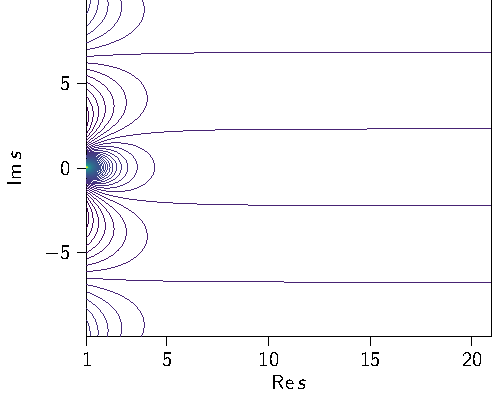
\includegraphics{figures/half_absolute_value_contour_plot.pdf}
        \vspace*{-3mm}
        \caption{Konturplot, Linien entsprechen gleichem Betrag.}
    \end{figure}
    }
    \only<2>{
    \begin{figure}
        \centering
        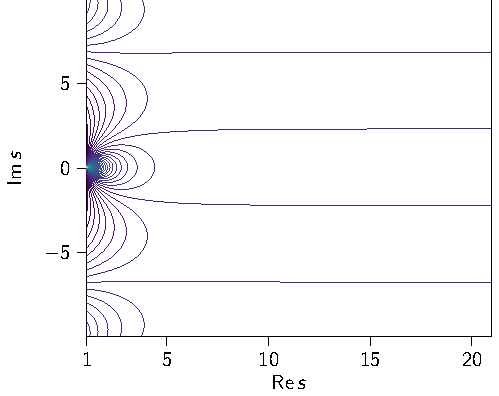
\includegraphics{figures/half_real_value_contour_plot.pdf}
        \vspace*{-3mm}
        \caption{Konturplot, Linien entsprechen gleichem Realteil.}
    \end{figure}
    }
    \only<3>{
    \begin{figure}
        \centering
        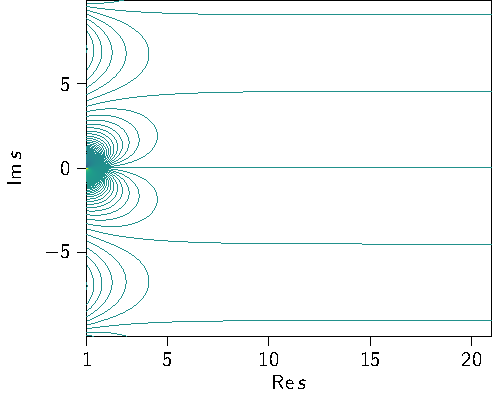
\includegraphics{figures/half_imag_value_contour_plot.pdf}
        \vspace*{-3mm}
        %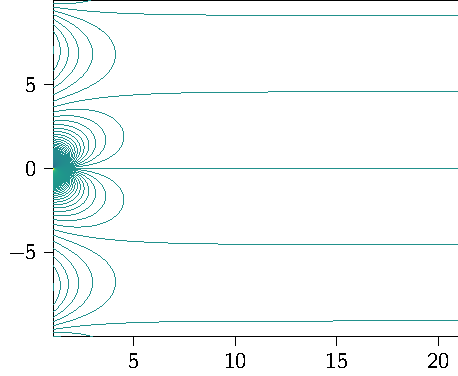
\includegraphics{figures/main-figure2.pdf}
        \caption{Konturplot, Linien entsprechen gleichem Imaginärteil.}
    \end{figure}
    }
\end{frame}
\begin{frame}
    \begin{lemma}[$\theta$-Funktion]
        Die Thetafunktion, gegeben durch
        \[
            \theta(z) = \sum_{n = -\infty}^{\infty} e^{i\pi n^2z},
        \] konvergiert für $\Im z > 0$.
    \end{lemma}
\end{frame}
\begin{frame}
    \begin{proof}
        \begin{align*}
            \visible<1->{\sum_{n = -\infty}^{\infty} \left|e^{i\pi n^2 (\Re z + i (\Im z)}\right| &= \sum_{n = -\infty}^{\infty} \left|e^{i\pi n^2 \Re z}\right|\cdot \left| e^{i \pi n^2 \cdot i (\Im z)}\right|\\}
            \visible<2->{&= \sum_{n = -\infty}^{\infty} e^{- \pi n^2 \Im z}\\}
            \visible<3->{&= \sum_{n = -N}^{N} e^{- \pi n^2 \Im z} + 2\cdot \sum_{n = N}^{\infty} e^{- \pi n^2 \Im z}\\}
            \visible<4>{&\leq \sum_{n = -N}^{N} e^{- \pi n^2 \Im z} + 2\cdot \sum_{n = N}^{\infty} \frac{1}{n^2}< \infty}
        \end{align*}
    \end{proof}
\end{frame}
\begin{frame}
    \begin{lemma}[$\theta$-Funktion]
        Die Thetafunktion, $\theta(z) = \sum_{n = -\infty}^{\infty} e^{i\pi n^2z}$, konvergiert für $\Im z > 0$.
    \end{lemma}
    \begin{behauptung}
        $\theta(z)$ erfüllt die Thetatransformationsformel ($\sqrt{\cdot}$ bezeichne den Zweig mit positivem Realteil): 
            \begin{align*}
                \theta(z) &= \theta\left(-\frac{1}{z}\right)\cdot \sqrt{\frac{i}{z}}\\
                \Leftrightarrow \theta(it) &= \theta\left(-\frac{1}{it}\right) \cdot \sqrt{\frac{i}{it}} = \theta\left(it^{-1}\right)\cdot t^{-\frac{1}{2}}.
            \end{align*}
    \end{behauptung}
\end{frame}
\begin{frame}
    \begin{lemma}
        Die Funktion 
        \[
            R_\infty(s) \coloneqq \int_1^\infty \frac{\theta(it)-1}{2} t^{s/2} \frac{\intd t}{t} = \int_1^\infty \sum_{n=1}^\infty e^{-\pi n^2 t} t^{s/2} \frac{\intd t}{t}
        \] ist ganz.
    \end{lemma}
\end{frame}
\begin{frame}
    \begin{block}{Beweis.}
        Abschätzen der Reihe ergibt
        \begin{align*}
            e^{\pi t} \cdot \sum_{n = 1}^{\infty} e^{-\pi t n^2} &= \sum_{n = 1}^{\infty} e^{-\pi t (n^2-1)}\stackrel{t \geq 1}{\leq} \sum_{n = 1}^{\infty} e^{-\pi (n^2-1)}\\
            \visible<2->{&= \sum_{n = 1}^{N} e^{-\pi (n^2-1)} + \sum_{n = N+1}^{\infty} e^{-\pi (n^2-1)}\\}
            \visible<3->{&\leq  \sum_{n = 1}^{N} e^{-\pi (n^2-1)} + \sum_{n = N+1}^{\infty} \frac{1}{n^2}\\}
            \visible<4->{&\leq B}
        \end{align*}
        \visible<5>{Also ist $\sum_{n = 1}^{\infty} e^{-\pi n^2 t} \leq B e^{-\pi t}$.}
    \end{block}
\end{frame}
\begin{frame}
    \begin{proof}
        \begin{align*}
            \int_1^\infty \sum_{n=1}^\infty e^{-\pi n^2 t} t^s \frac{\intd t}{t} &\leq B \cdot \int_1^\infty e^{-\pi t} t^{s+1} \frac{\intd t}{t^2}
            \visible<2->{\intertext{$\exists a(s):\ \forall \alpha > a: e^{-\pi \alpha} < \alpha^{-s+1}$}}
            \visible<3->{&= B \cdot \int_1^a e^{-\pi t} t^{s+1} \frac{\intd t}{t^2} + B\cdot \int_a^\infty e^{-\pi t} t^{s+1} \frac{\intd t}{t^2}\\}
            \visible<4->{&\leq B \cdot C(s) + B\cdot \int_a^\infty \frac{\intd t}{t^2}\\}
            \visible<5->{&\leq B\cdot C(s) + \frac{B}{a(s)} < \infty}
        \end{align*}
    \end{proof}
\end{frame}
\begin{frame}
    \begin{lemma}
        Die Riemannsche $\zeta$-Funktion besitzt eine analytische Fortsetzung auf $\C\setminus\{1\}$, wobei an der Stelle 1 eine einfache Polstelle vorliegt. Außerdem genügt 
        \[\xi(s) \coloneqq \pi^{-\frac{s}{2}} \Gamma\left(\frac{s}{2}\right)\zeta(s)\] der Funktionalgleichung $\xi(s) = \xi(1-s)$.
    \end{lemma}
\end{frame}
\begin{frame}
    \begin{block}{Beweis.}
        Sei $\Re s > 1$.
        \begin{align*}
            \Gamma(s) &= \int_0^\infty e^{-t} t^s \frac{\intd t}{t}&&\left|t \mapsto \pi n^2t\right.\\
            \visible<2->{&= \int_0^\infty e^{-\pi n^2t}(\pi n^2 t)^s \frac{\intd t}{t} &&\left|\cdot \pi^{-s} \cdot n^{-2s}\right.\\}
            \visible<4->{\sum_{n = 1}^{\infty}}\visible<3->{\pi^{-s} \Gamma(s)n^{-2s}&= }\only<4->{\sum_{n = 1}^{\infty}}\visible<3->{\int_0^\infty e^{-\pi n^2 t} t^s \frac{\intd t}{t}&&\left|\sum_{n = 1}^{\infty},\; s\mapsto s/2\right.\\}
            \alt<6>{\invisible<1->{\sum_{n=1}^{\infty}n^{-s}}}{\invisible<1->{\zeta(s)}}\visible<5->{\pi^{-s/2} \Gamma(s/2)\alt<6>{\zeta(s)}{\sum_{n=1}^{\infty}n^{-s}} &= \sum_{n=1}^\infty \int_0^\infty e^{-\pi n^2 t}t^{s/2} \frac{\intd t}{t}}
        \end{align*}
    \end{block}
\end{frame}
\begin{frame}
    \begin{block}{Beweis.}%
    Wegen
    \begin{align*}
        \sum_{n = 1}^{\infty} \left|\int_0^\infty e^{-\pi n^2 t}t^{s/2} \frac{\intd t}{t}\right| &\leq \sum_{n = 1}^{\infty} \int_0^\infty e^{-\pi n^2 t}t^{\Re s/2} \frac{\intd t}{t}\\
        &= \pi^{- \Re s/2} \Gamma(\Re s/2)\zeta(\Re s)\\
        &< \infty
    \end{align*}
    gilt nach dem Satz von Fubini/Tonelli für absolut konvergente Reihen
    \[
        \sum_{n = 1}^{\infty} \int_0^\infty e^{-\pi n^2 t}t^{s/2} \frac{\intd t}{t} = \int_0^\infty \sum_{n = 1}^{\infty} e^{-\pi n^2 t}t^{s/2} \frac{\intd t}{t}.
    \]
    \end{block}
\end{frame}
\begin{frame}
\begin{block}{Beweis.}
    \begin{align*}
        \pi^{-s/2} \Gamma(s/2)\zeta(s) &= \alt<1>{\sum_{n = 1}^{\infty} \int_0^\infty}{\int_0^\infty \sum_{n = 1}^{\infty}} e^{-\pi n^2 t}t^{s/2} \frac{\intd t}{t}\\
        \visible<3->{&= \int_0^\infty \frac{\theta(it)-1}{2} t^{s/2} \frac{\intd t}{t}\\}
        \visible<4->{&= \underbrace{\int_0^1 \frac{\theta(it)-1}{2} t^{s/2} \frac{\intd t}{t}}_{R_0(s)} + \underbrace{\int_1^\infty \frac{\theta(it)-1}{2} t^{s/2} \frac{\intd t}{t}}_{R_\infty(s)}\\}
        \visible<5->{&= R_0(s) + R_\infty(s)}
    \end{align*}
\end{block}
\end{frame}

\begin{frame}
\begin{block}{Beweis.}
    \begin{align*}
        R_0(s) &= \int_0^1 \frac{\theta(it)-1}{2} t^{s/2} \frac{\intd t}{t}\invisible<1->{\hspace*{2.2cm}}&&\left|\theta(it) = \theta(it^{-1})\cdot t^{-\frac{1}{2}}\right.\\
        \visible<2->{&= \only<3->{-}\alt<-2>{\int_0^1}{\int_1^0} \frac{\theta\left(it^{-1}\right)\cdot t^{-\frac{1}{2}}-1}{2} t^{s/2\only<4->{+1}} \frac{\intd t}{t\only<4->{^2}}&&\left|u = \frac{1}{t},\; \intd u = \frac{-1}{t^2}\intd t\right.\\}
        \visible<5->{&= \int_1^\infty \frac{\theta\left(iu\right)\cdot u^{\frac{1}{2}}-1}{2} u^{-s/2-1} \intd u\\}
        \visible<6->{&= \int_1^\infty \frac{\theta\left(it\right)\cdot t^{\frac{1}{2}}-1}{2} t^{-s/2} \frac{\intd t}{t}}
    \end{align*}
\end{block}
\end{frame}
\begin{frame}
\begin{block}{Beweis.}
    \begin{align*}
        R_0(s) &= \alt<3->{\int_1^\infty 
        \alt<3>{\frac{\theta\left(it\right)\cdot t^{\frac{1}{2}}-t^{\frac{1}{2}}}{2}\cdot t^{-s/2}}{\frac{\theta\left(it\right)-1}{2}\cdot t^{\frac{1-s}{2}}}\only<4>{}\frac{\intd t}{t} + \int_1^\infty \frac{t^{\frac{1}{2}} -1}{2} t^{-s/2} \frac{\intd t}{t}}{\int_1^\infty \frac{\theta\left(it\right)\cdot t^{\frac{1}{2}}\only<2->{-t^{\frac{1}{2}} + t^{\frac{1}{2}}}-1}{2} t^{-s/2} \frac{\intd t}{t}}\\
        \visible<5->{&= R_\infty\left(1-s\right) + \int_1^\infty \frac{1}{2}t^{\frac{1-s}{2}} \frac{\intd t}{t} - \int_1^{\infty} \frac{1}{2} t^{-s/2} \frac{\intd t}{t}\hspace*{1.4cm}\\}
        \visible<6->{&= R_\infty(1-s) + \alt<6>{\frac{1}{2}\frac{2}{1-s}}{\frac{1}{1-s}}t^{\frac{1-s}{2}}\bigg|_1^\infty + \alt<6>{\frac{1}{2}\frac{2}{s}}{\frac{1}{s}}t^{-\frac{s}{2}}\bigg|_1^\infty\\}
        \visible<8->{&= R_\infty\left(1-s\right) - \frac{1}{1-s} - \frac{1}{s}\\}
    \end{align*}
\end{block}
\end{frame}
\begin{frame}
\begin{block}{Beweis.}
    \vspace*{-0.5cm}
    \begin{align*}
        \pi^{-s/2} \Gamma(s/2)\zeta(s) &= R_\infty(s) + R_0(s)\\
        \visible<3->{\xi(s)}\visible<2->{&= R_\infty(s) + R_\infty(1-s) - \frac{1}{s} - \frac{1}{1-s}}
    \end{align*}%
    \begin{itemize}
        \item<4-> $R_\infty$ ist ganz
        \item<5-> $\xi$ ist holomorph auf $\C \setminus\{0,1\}$.
        \item<6-> $\xi$ genügt der Funktionalgleichung $\xi(s) = \xi(1-s)$
    \end{itemize}
\end{block}
\end{frame}
\begin{frame}
    \begin{block}{Beweis.}
        \begin{align*}
            \pi^{-s/2} \Gamma(s/2)\zeta(s) &= \xi(s)\\
            \visible<2->{\zeta(s) &= \frac{\pi^{s/2}}{\Gamma(s/2)}\xi(s)}
        \end{align*}
        \visible<3->{$\Gamma$ ist meromorph auf $\C$ und besitzt keine Nullstellen.\\}
        \visible<4->{$\implies$ $\frac{\pi^{s/2}}{\Gamma(s/2)}$ ist holomorph auf $\C$.\\}
        \visible<5->{$\implies$ $\frac{\pi^{s/2}}{\Gamma(s/2)}\xi(s)$ ist holomorph auf $\C\setminus\{0,1\}$.}
    \end{block}
\end{frame}
\begin{frame}
    \begin{block}{Beweis.}
        \begin{align*}
            & \lim\limits_{s \to 0} \frac{\pi^{s/2}}{\Gamma(s/2)}\bigg(\underbrace{R_\infty(s) + R_\infty(1-s) - \frac{1}{1-s}}_{\implies \text{beschränkt für } s \to 0} - \frac{1}{s}\bigg)\\
            \visible<2->{\intertext{Wegen $\lim\limits_{s \to 0} \Gamma(s/2) = \infty$ erhalten wir}}
            \visible<3->{=& 0 - \lim\limits_{s \to 0} \frac{\pi^{s/2}}{s\cdot \Gamma(s/2)} = - \lim\limits_{s \to 0} \frac{\pi^{s/2}}{2\cdot s/2\cdot \Gamma(s/2)}\\}
            \visible<4->{=& -\lim\limits_{s \to 0} \frac{\pi^{s/2}}{2\cdot \Gamma(s/2 + 1)}= -\frac{\pi^0}{2\cdot \Gamma(1)} = -\frac{1}{2}}
        \end{align*}
    \end{block}
\end{frame}
\begin{frame}
    \begin{block}{Beweis.}
        Die Funktion \[
            \frac{\pi^{s/2}}{\Gamma(s/2)}\left(R_\infty(s) + R_\infty(1-s) - \frac{1}{s} - \frac{1}{1-s}\right)
        \] ist daher
        \begin{itemize}
            \item<2-> holomorph auf $\C \setminus \{1\}$. 
            \item<3-> stimmt für $\Re s > 1$ mit $\zeta(s)$ überein
        \end{itemize}
        \visible<4->{$\implies$ stellt die gesuchte analytische Fortsetzung für die Riemannsche $\zeta$-Funktion dar!!!}
    \end{block}
\end{frame}
\begin{frame}
    \begin{block}{Exkurs.}
        Es gilt die Duplikationsformel und der Ergänzungssatz: 
        \[
            \frac{\Gamma\left(\frac{1-s}{2}\right)}{\Gamma\left(\frac{s}{2}\right)} = \frac{\Gamma\left(\frac{1-s}{2}\right) \cdot \Gamma\left(1-\frac{s}{2}\right)}{\Gamma\left(\frac{s}{2}\right)\cdot \Gamma\left(1-\frac{s}{2}\right)} = \frac{\sin\left(\frac{\pi \cdot s}{2}\right)}{\pi} \cdot \frac{\sqrt{\pi}}{2^{1-s-1}}\cdot \Gamma(1-s)
        \]
        \begin{align*}
            \xi(s) &= \xi(1-s)\\
            \pi^{-\frac{s}{2}} \Gamma\left(\frac{s}{2}\right)\zeta(s) &= \pi^\frac{s-1}{2} \Gamma\left(\frac{1-s}{2}\right)\zeta(1-s)\\
            \zeta(s) &= \pi^{s-1}\cdot \sqrt{\pi} \frac{\Gamma\left(\frac{1-s}{2}\right)}{\Gamma\left(\frac{s}{2}\right)}\zeta(1-s)\\
            &= \pi^{s-1} \cdot 2^s \cdot \sin\left(\frac{\pi s}{2}\right)\Gamma(1-s)\zeta(1-s)
        \end{align*}
    \end{block}
\end{frame}
\begin{frame}
    \begin{block}{Beispiel}
        \[
            \zeta(s) = \pi^{s-1} \cdot 2^s \cdot \sin\left(\frac{\pi s}{2}\right)\Gamma(1-s)\zeta(1-s)
        \]
        \[
            \zeta(-1) = \pi^{-2} \cdot 2^{-1} \cdot \sin\left(\frac{-\pi}{2}\right)\Gamma(2)\zeta(2) = \frac{1}{2\pi^2}\cdot -1 \cdot 1 \cdot \frac{\pi^2}{6} = -\frac{1}{12}
        \]
        \visible<2->{\[
           -\frac{1}{12} = \zeta(-1)\ \text{\glqq}=\text{\grqq}\ \sum_{n = 1}^{\infty} \frac{1}{n^{-1}} = 1 + 2 + 3 + \dots  
        \]}
    \end{block}
\end{frame}
\begin{frame}[label=current]
    \only<1>{
    \begin{figure}
        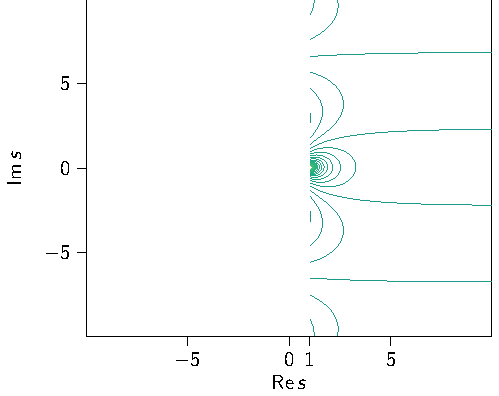
\includegraphics{figures/half_absolute_value_contour_for_overlays_plot.pdf}
        \vspace*{-4mm}
        \caption{Konturplot, Linien entsprechen gleichem Betrag}
    \end{figure}
    }
    \only<2>{
        \begin{figure}
            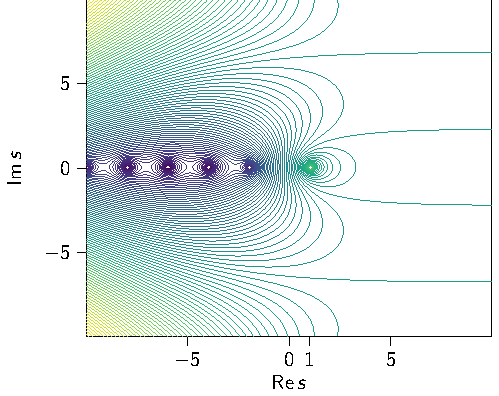
\includegraphics{figures/full_absolute_value_contour_for_overlays_plot.pdf}
            \vspace*{-4mm}
            \caption{Konturplot, Linien entsprechen gleichem Betrag}
        \end{figure}
    }
\end{frame}
\begin{frame}[label=current]%
    \begin{figure}%
        \begin{tikzpicture}
        \temporal<2>{
                \node[anchor=south west,inner sep=0] (image) at (0,0) {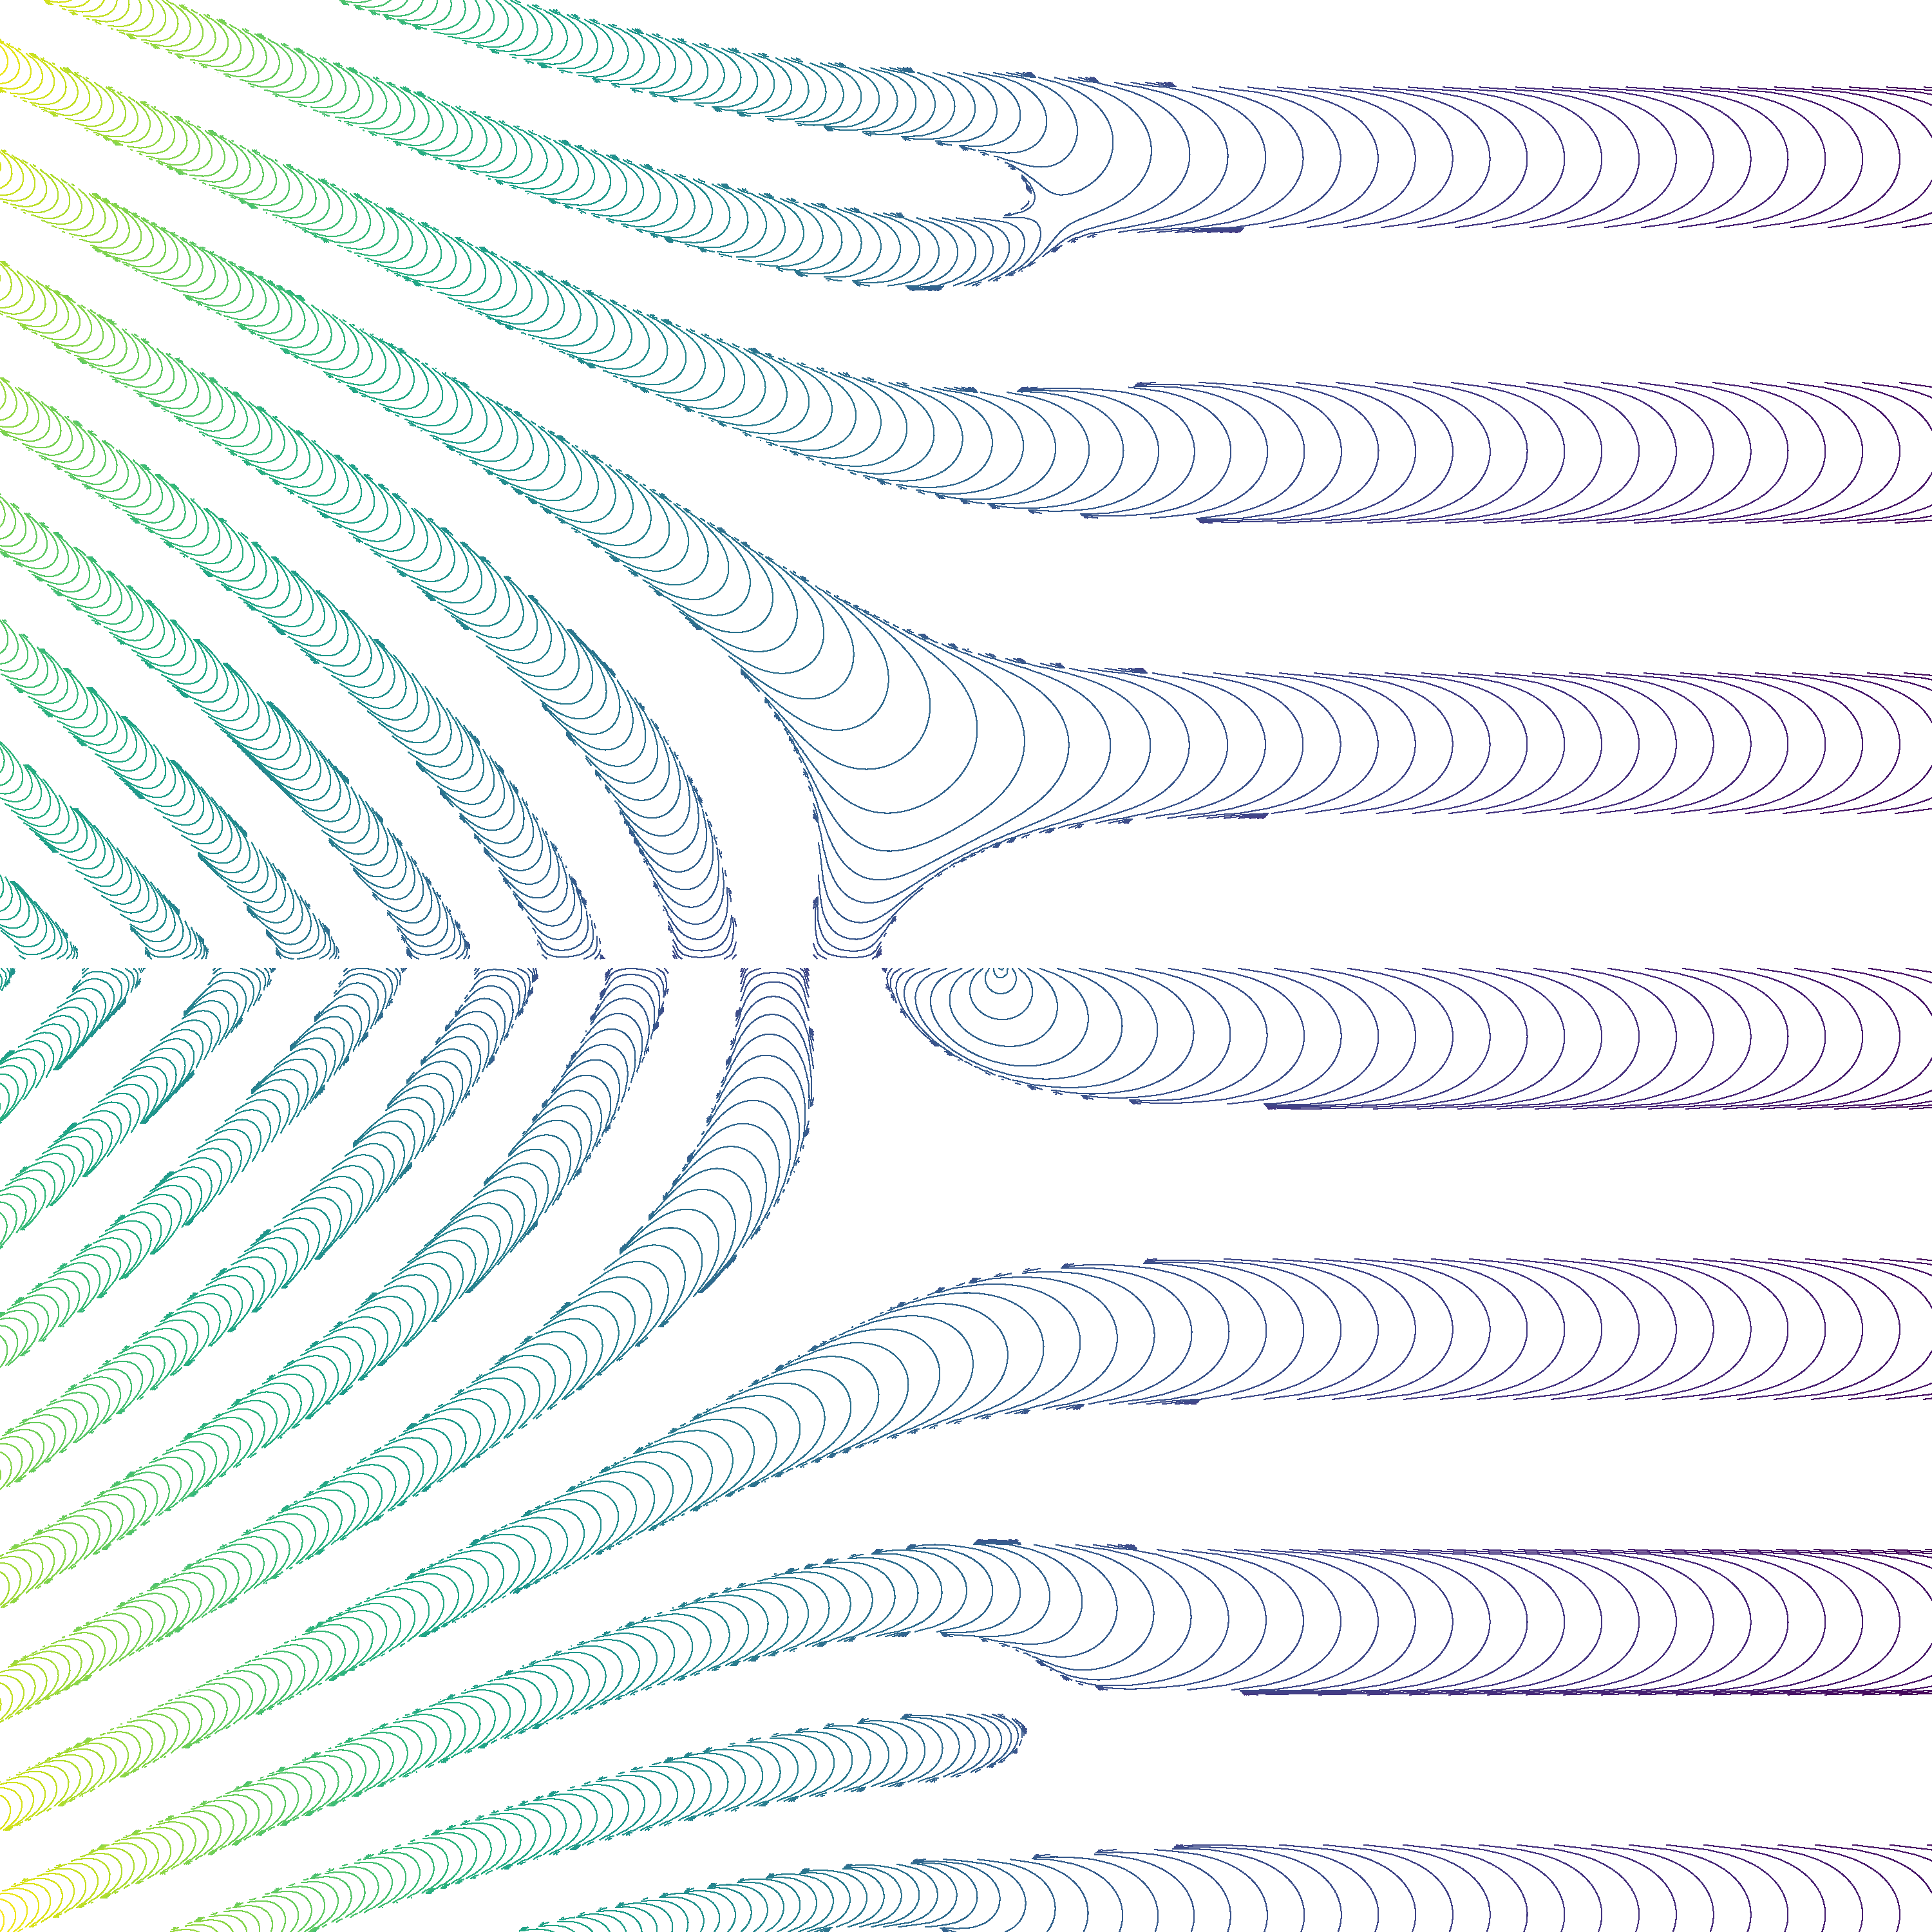
\includegraphics[width=0.55\textwidth]{figures/3030imag_contour_py.pdf}};
            }{
                \node[anchor=south west,inner sep=0] (image) at (0,0) {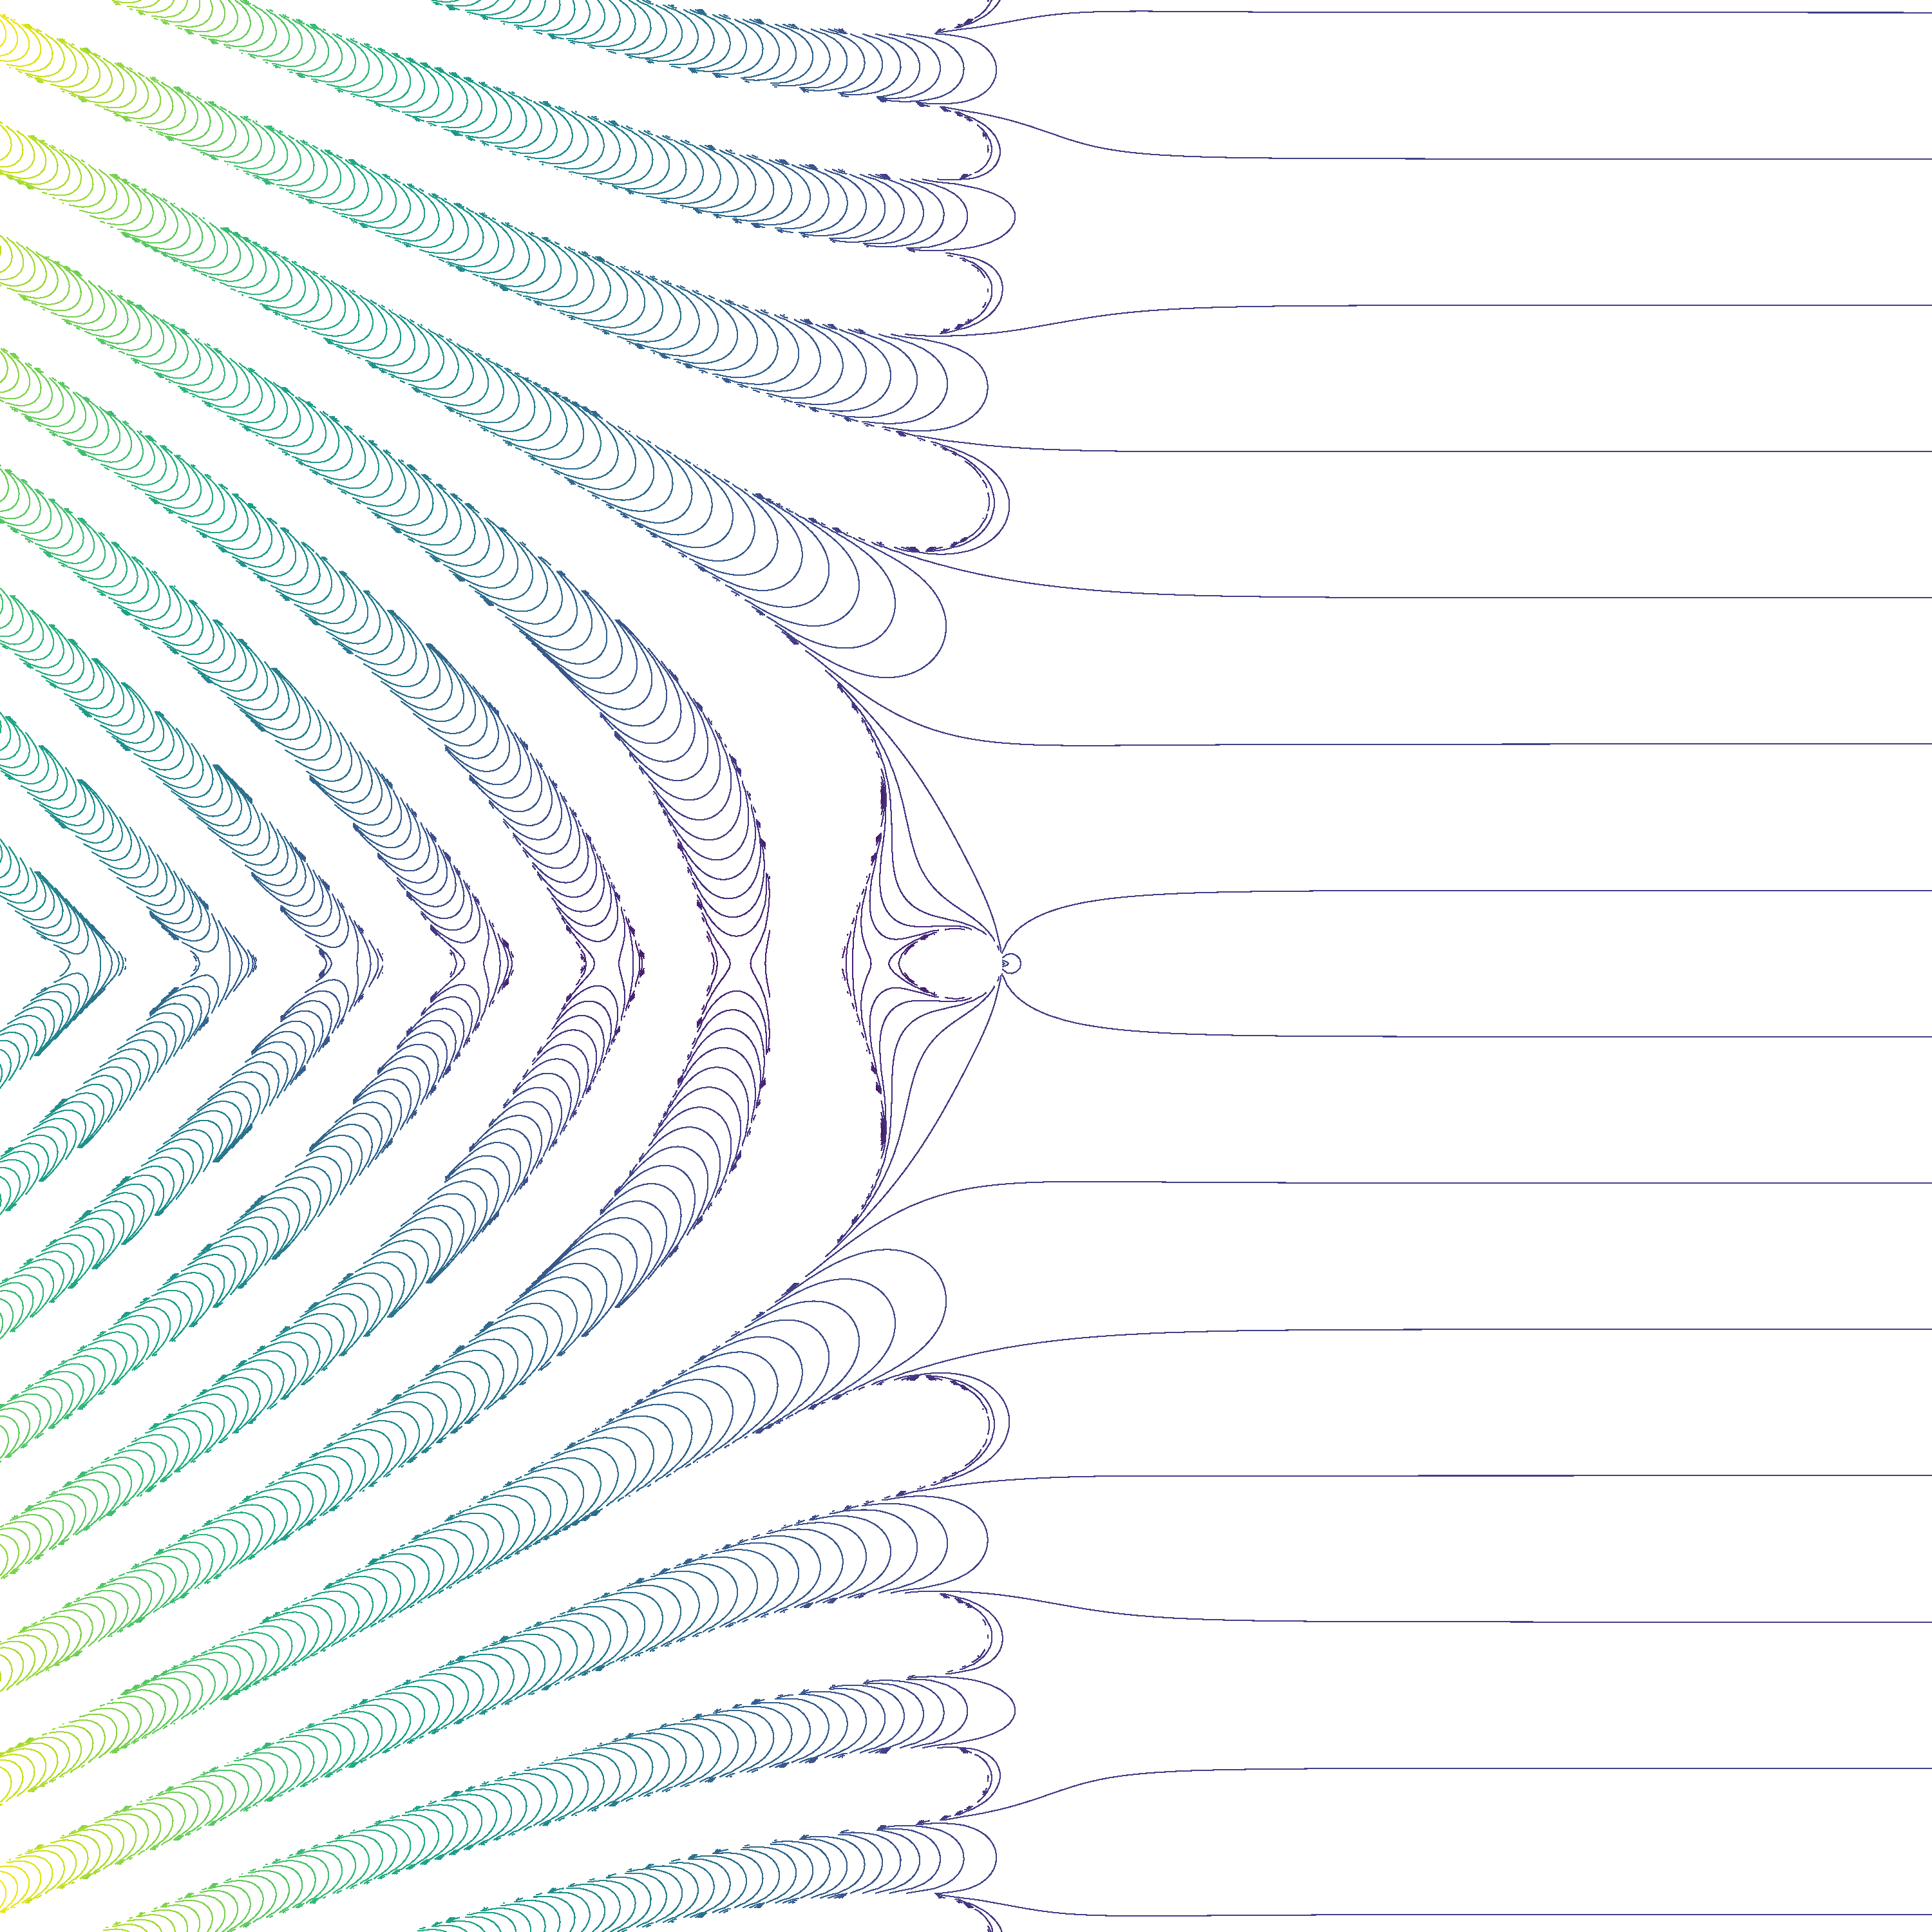
\includegraphics[width=0.55\textwidth]{figures/3030real_contour_py.pdf}};
            }{
                \node[anchor=south west,inner sep=0] (image) at (0,0) {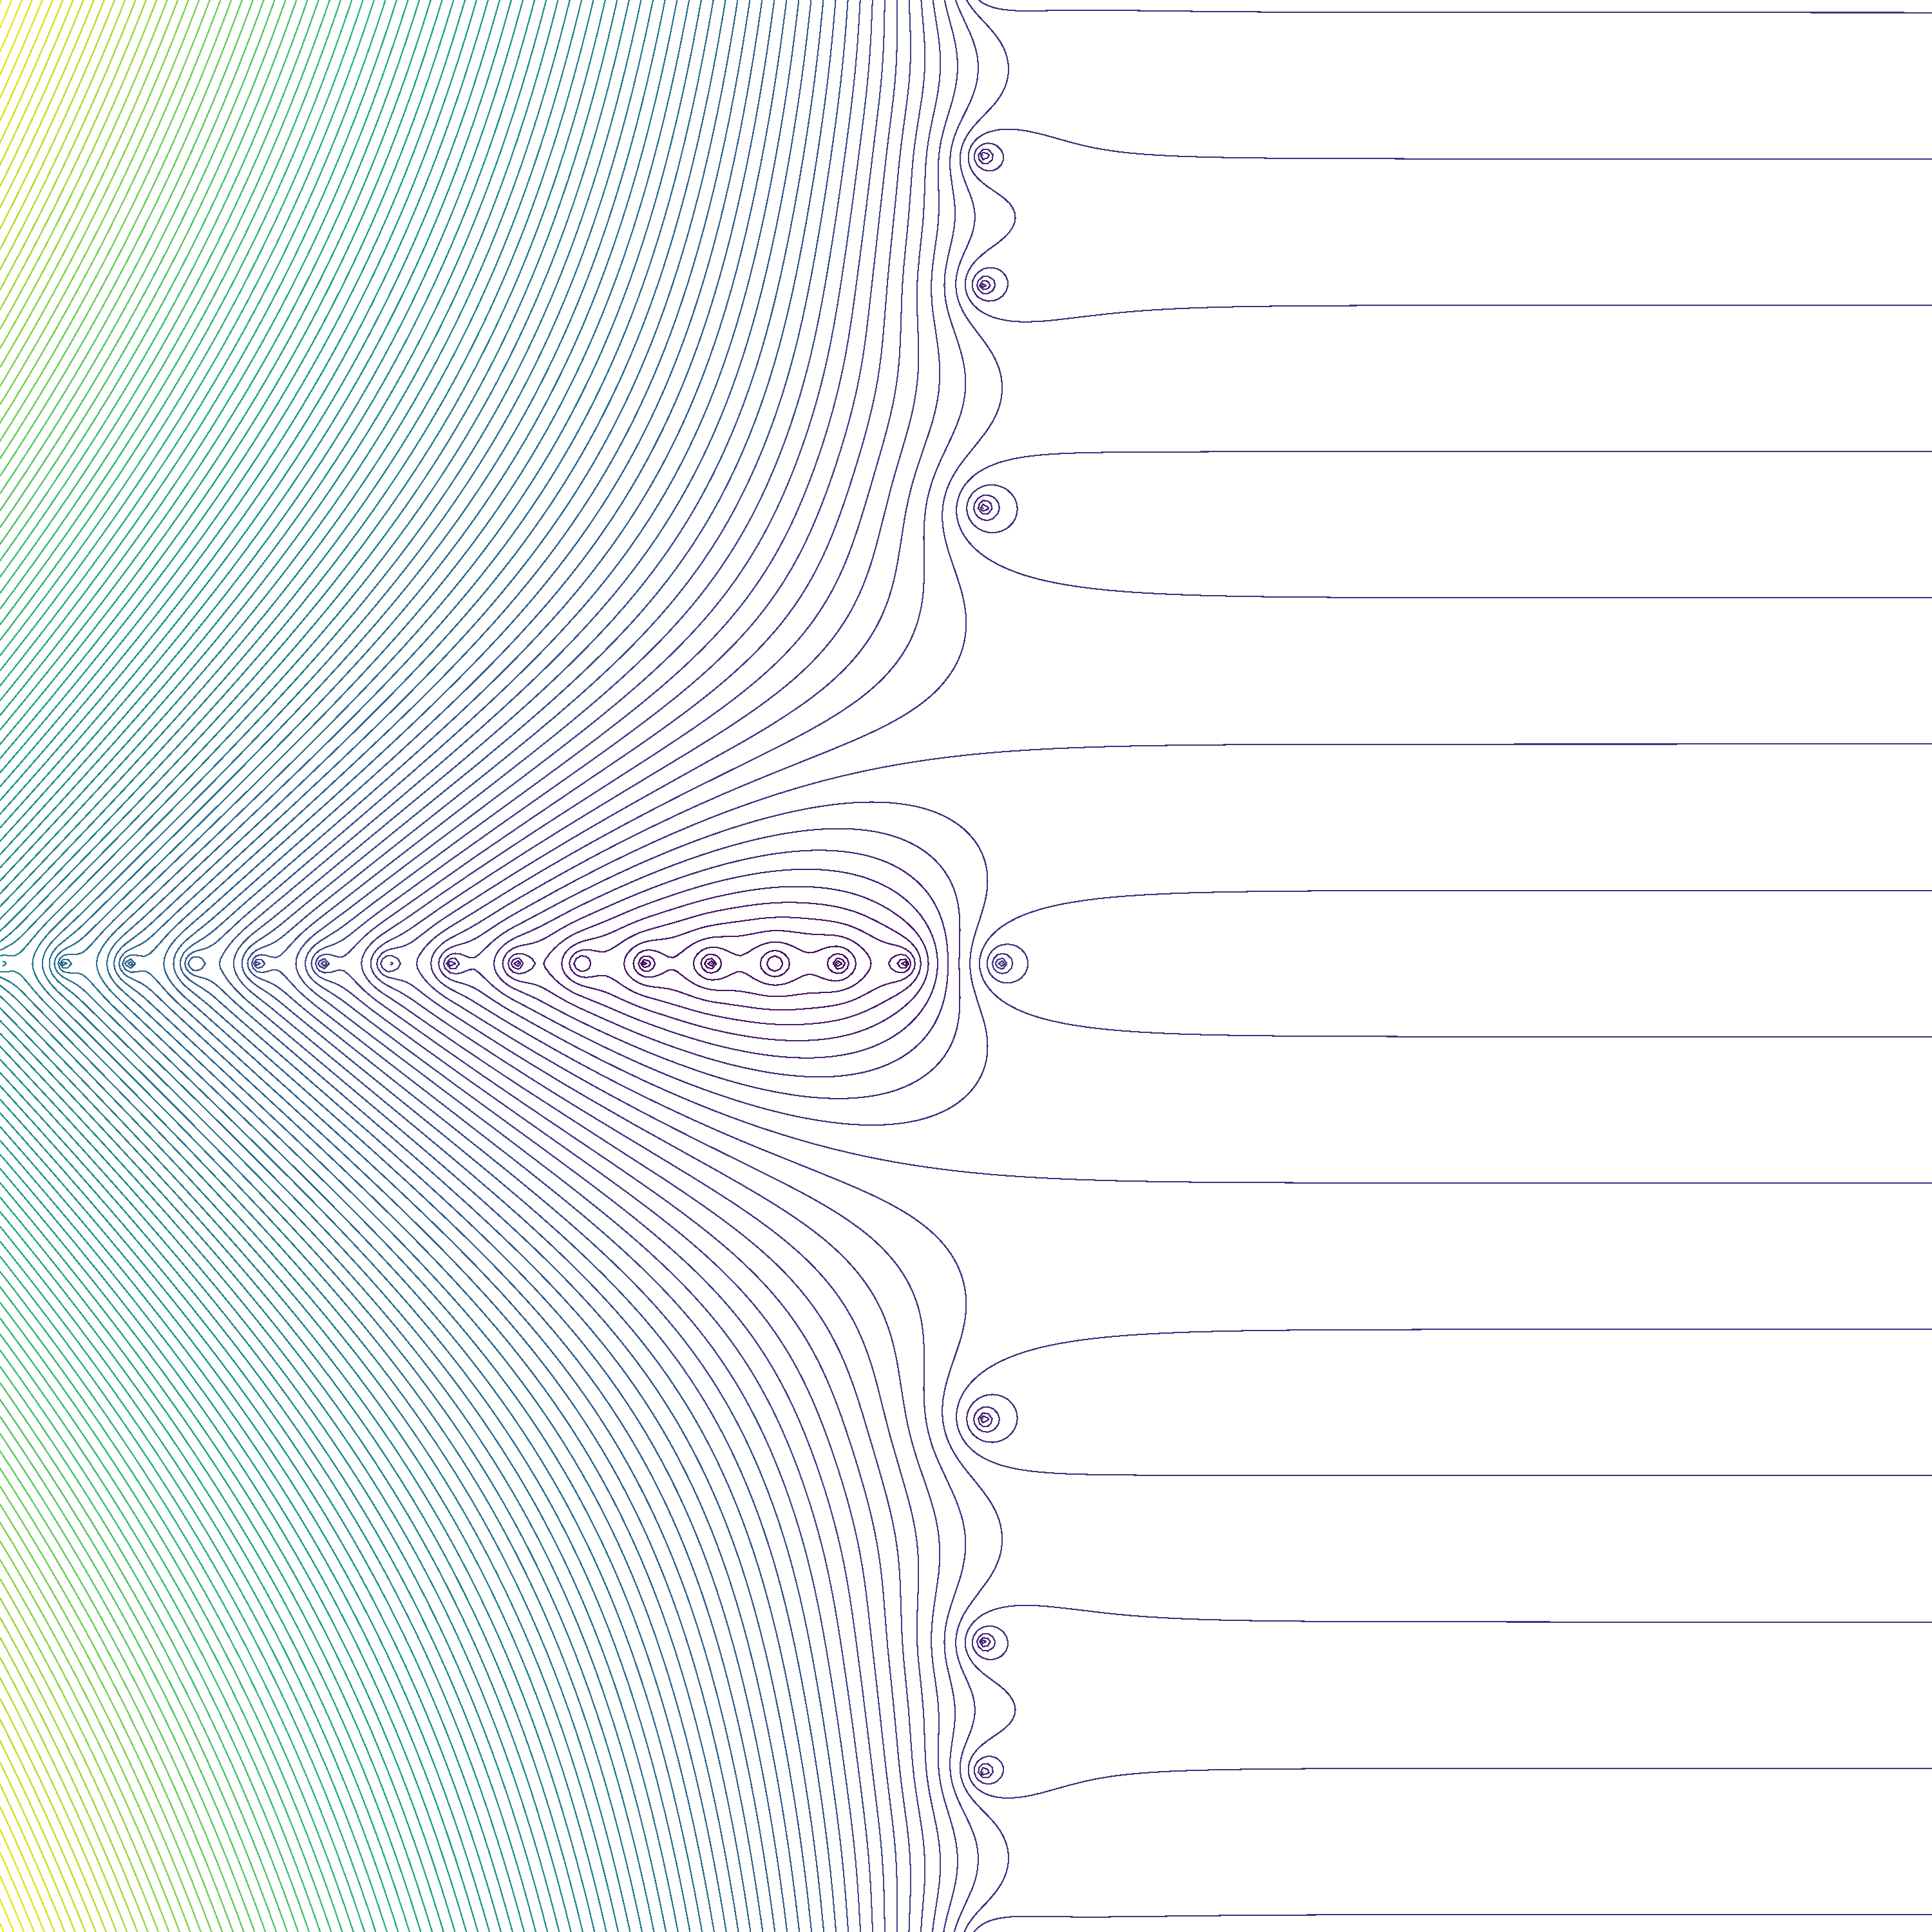
\includegraphics[width=0.55\textwidth]{figures/3030abs_contour_py.pdf}};
            }
        \begin{scope}[x={(image.south east)},y={(image.north west)}]
            %\draw[help lines,xstep=.1,ystep=.1] (0,0) grid (1,1);
            \foreach \y in {-20,-10,...,20} {
                \node [anchor=east] at (0,\y/60+0.5) {$\y$}; 
                \draw (0,\y/60+0.5) -- (-1mm,\y/60+0.5);
                }
            \foreach \x in {-20,-10,0,1,10,20} { 
                \node [anchor=north] at (\x/56+0.5,0) {$\x$}; 
                \draw (\x/60+0.5,0) -- (\x/60+0.5,-1mm);
                }
            \node[rotate=90] (ylabel) at (-.12,0.5) {$\operatorname{\Im s}$};
            \node (xlabel) at (0.5,-.115) {$\operatorname{\Re s}$};
            \draw[very thin] (0,0) rectangle (1,1);
            \only<4->{\fill[color=white, opacity=0.8] (0.52,0) rectangle (1,1);}
        \end{scope}
    \end{tikzpicture}%
    \vspace*{-13pt}
    \caption{\temporal<2>{Imaginärteil}{Realteil}{Betrag} der $\zeta$-Funktion}
    \end{figure}
\end{frame}
\section{Nullstellen, Riemannsche Hypothese}
\begin{frame}
    \begin{figure}%
        \begin{tikzpicture}
        \only<1>{\node[anchor=south west,inner sep=0] (image) at (0,0) {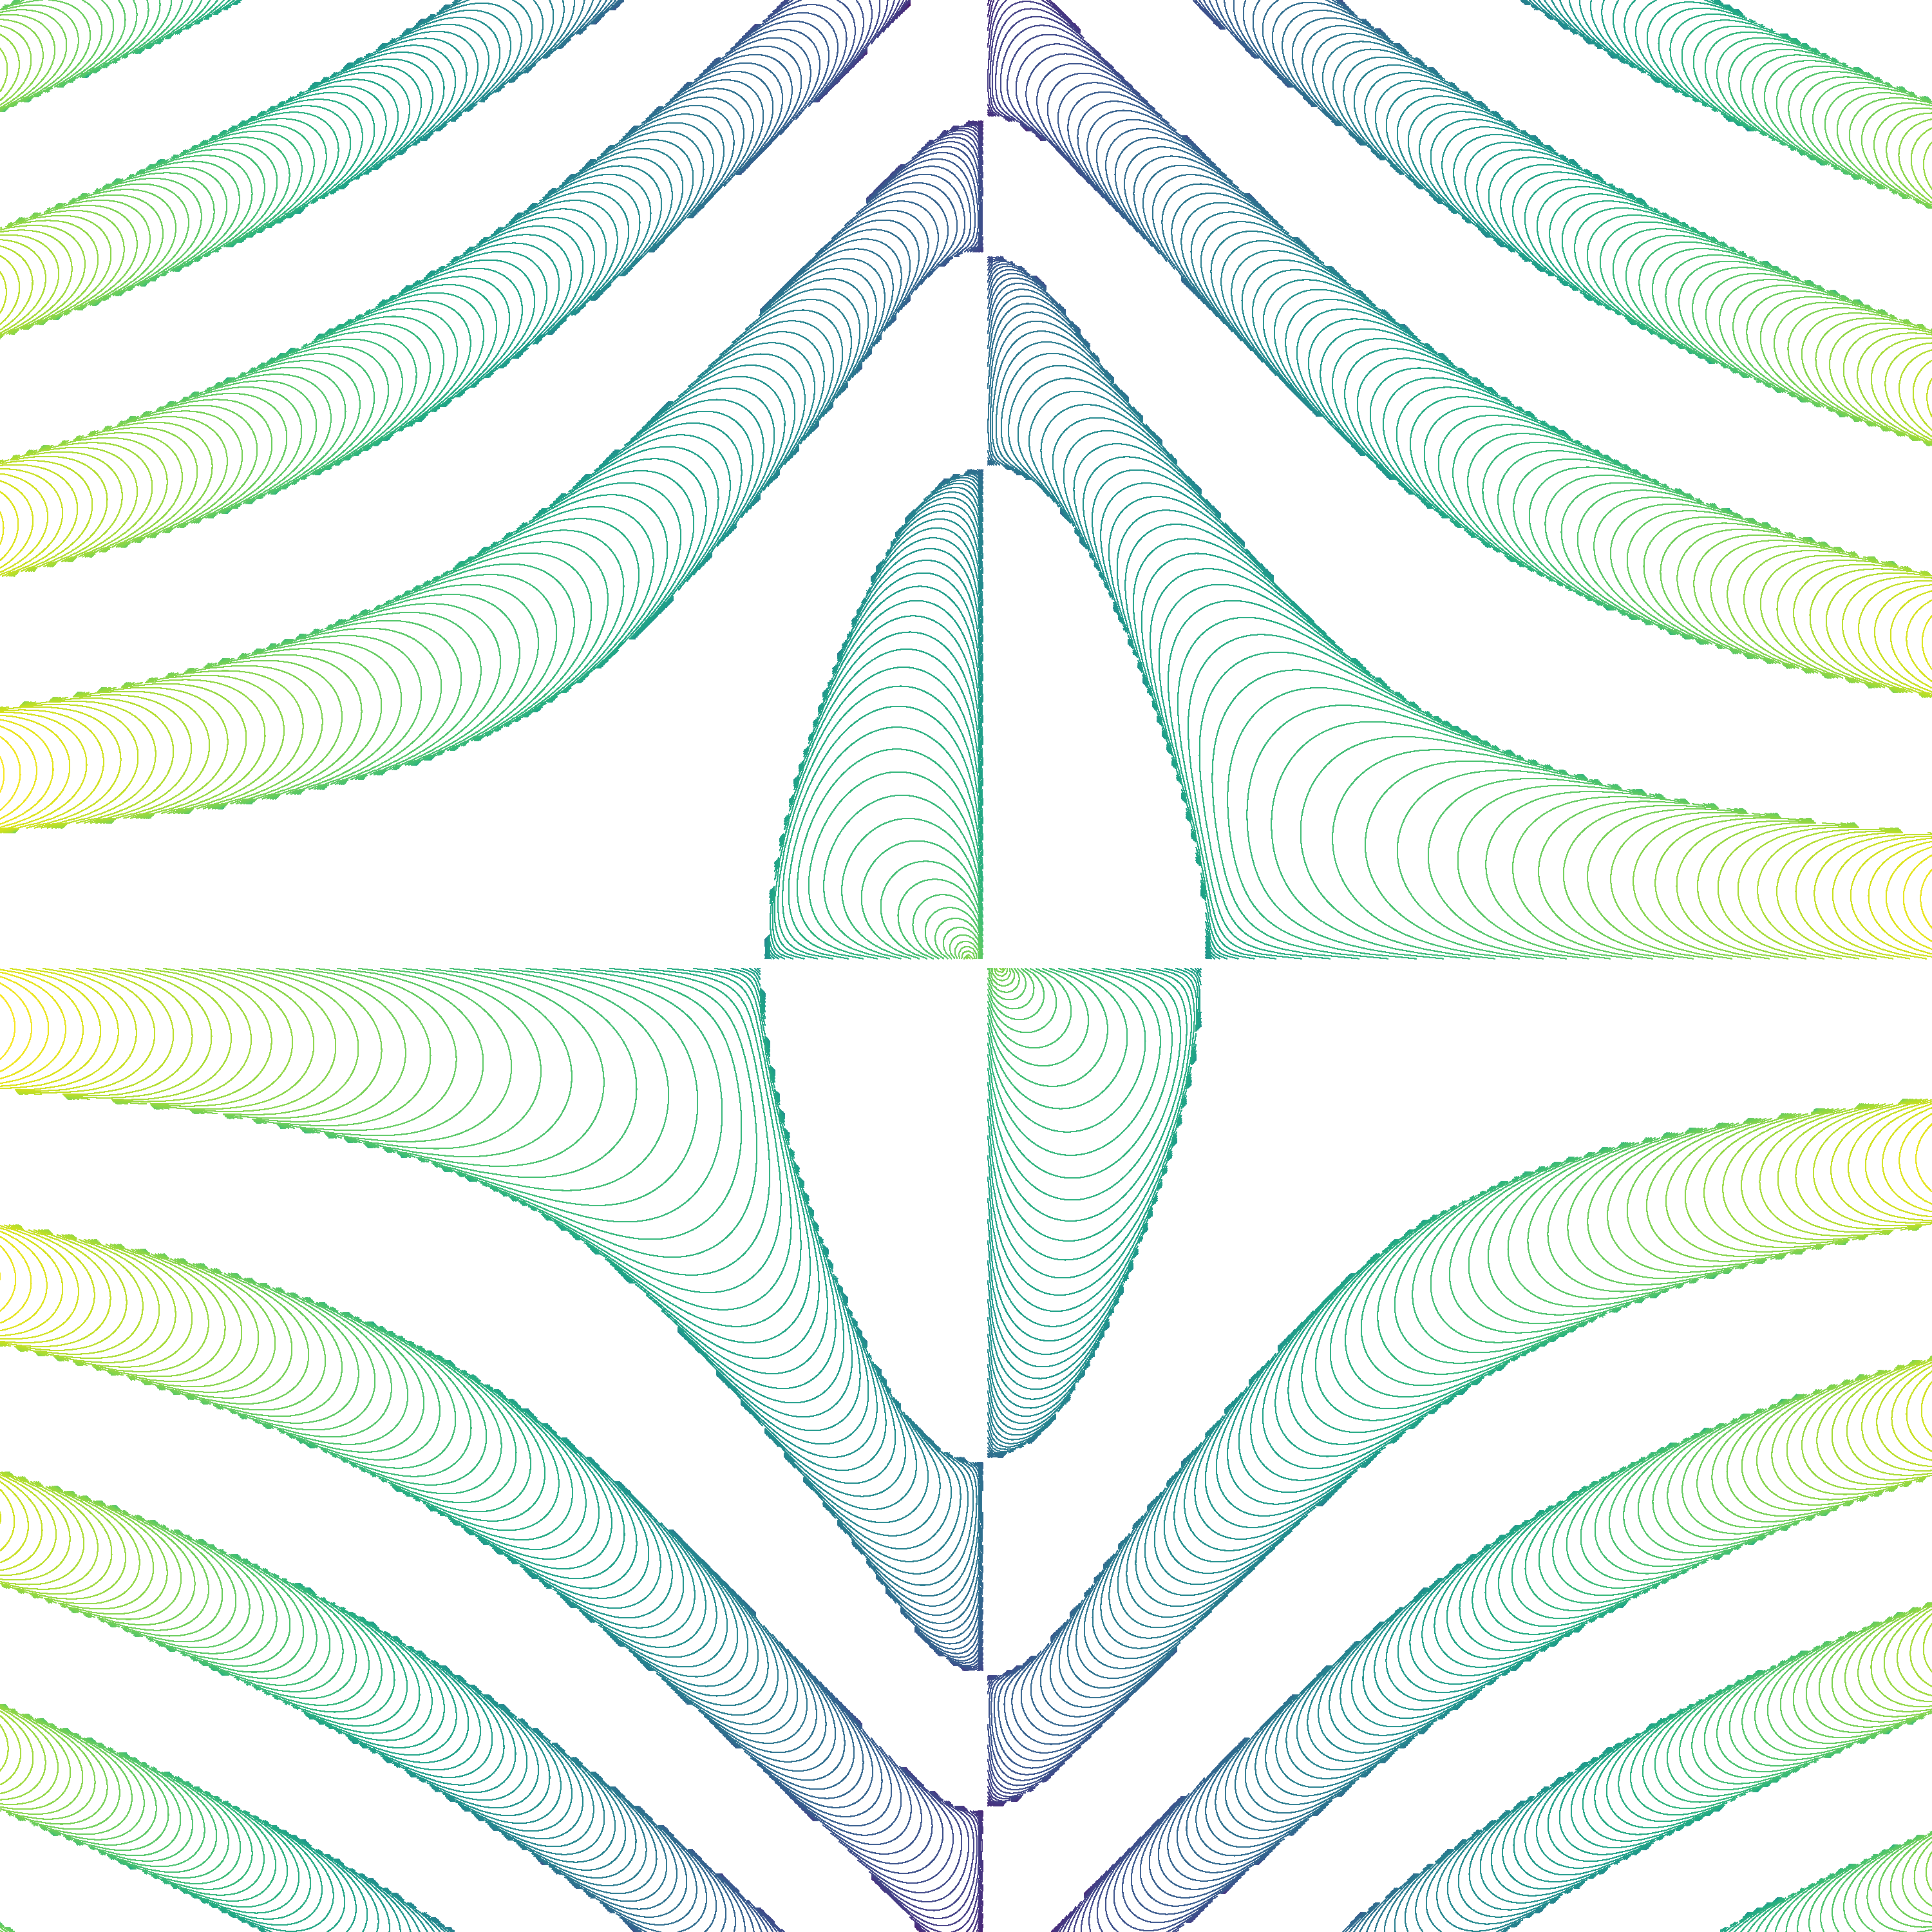
\includegraphics[width=0.55\textwidth]{figures/3030imag_contour_xi.pdf}};}
        \only<2>{\node[anchor=south west,inner sep=0] (image) at (0,0) {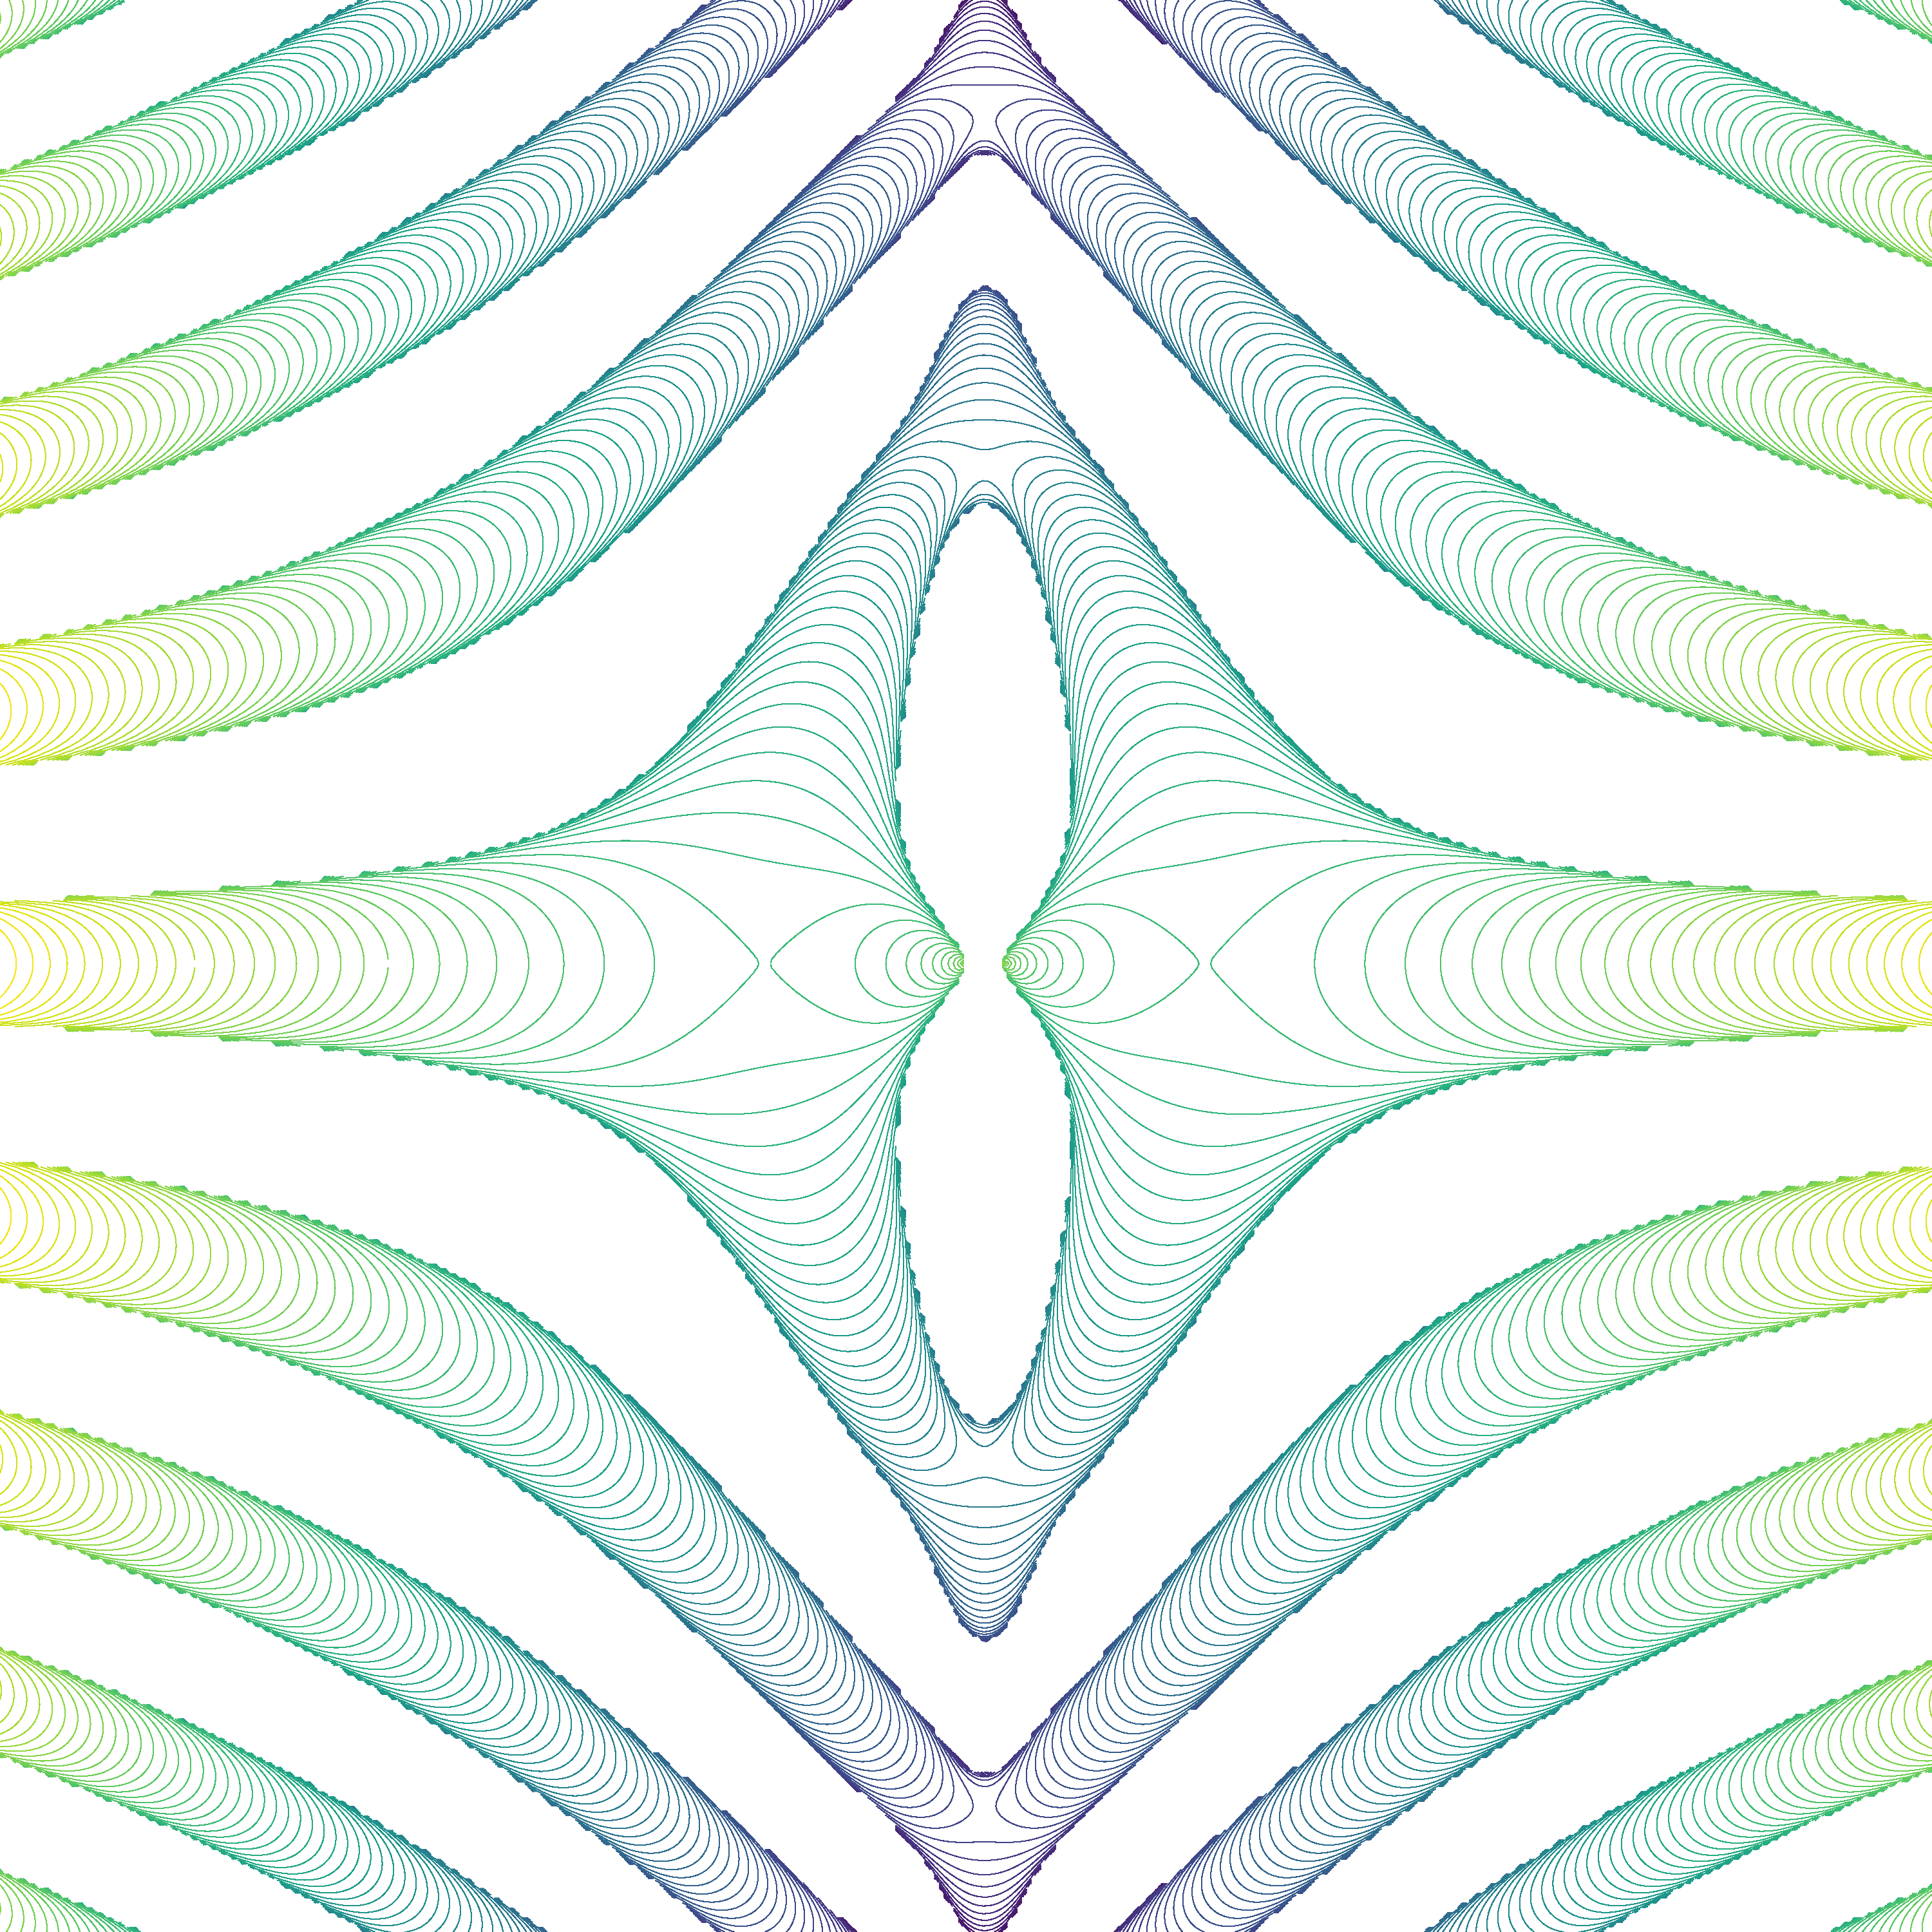
\includegraphics[width=0.55\textwidth]{figures/3030real_contour_xi.pdf}};}
        \only<3->{\node[anchor=south west,inner sep=0] (image) at (0,0) {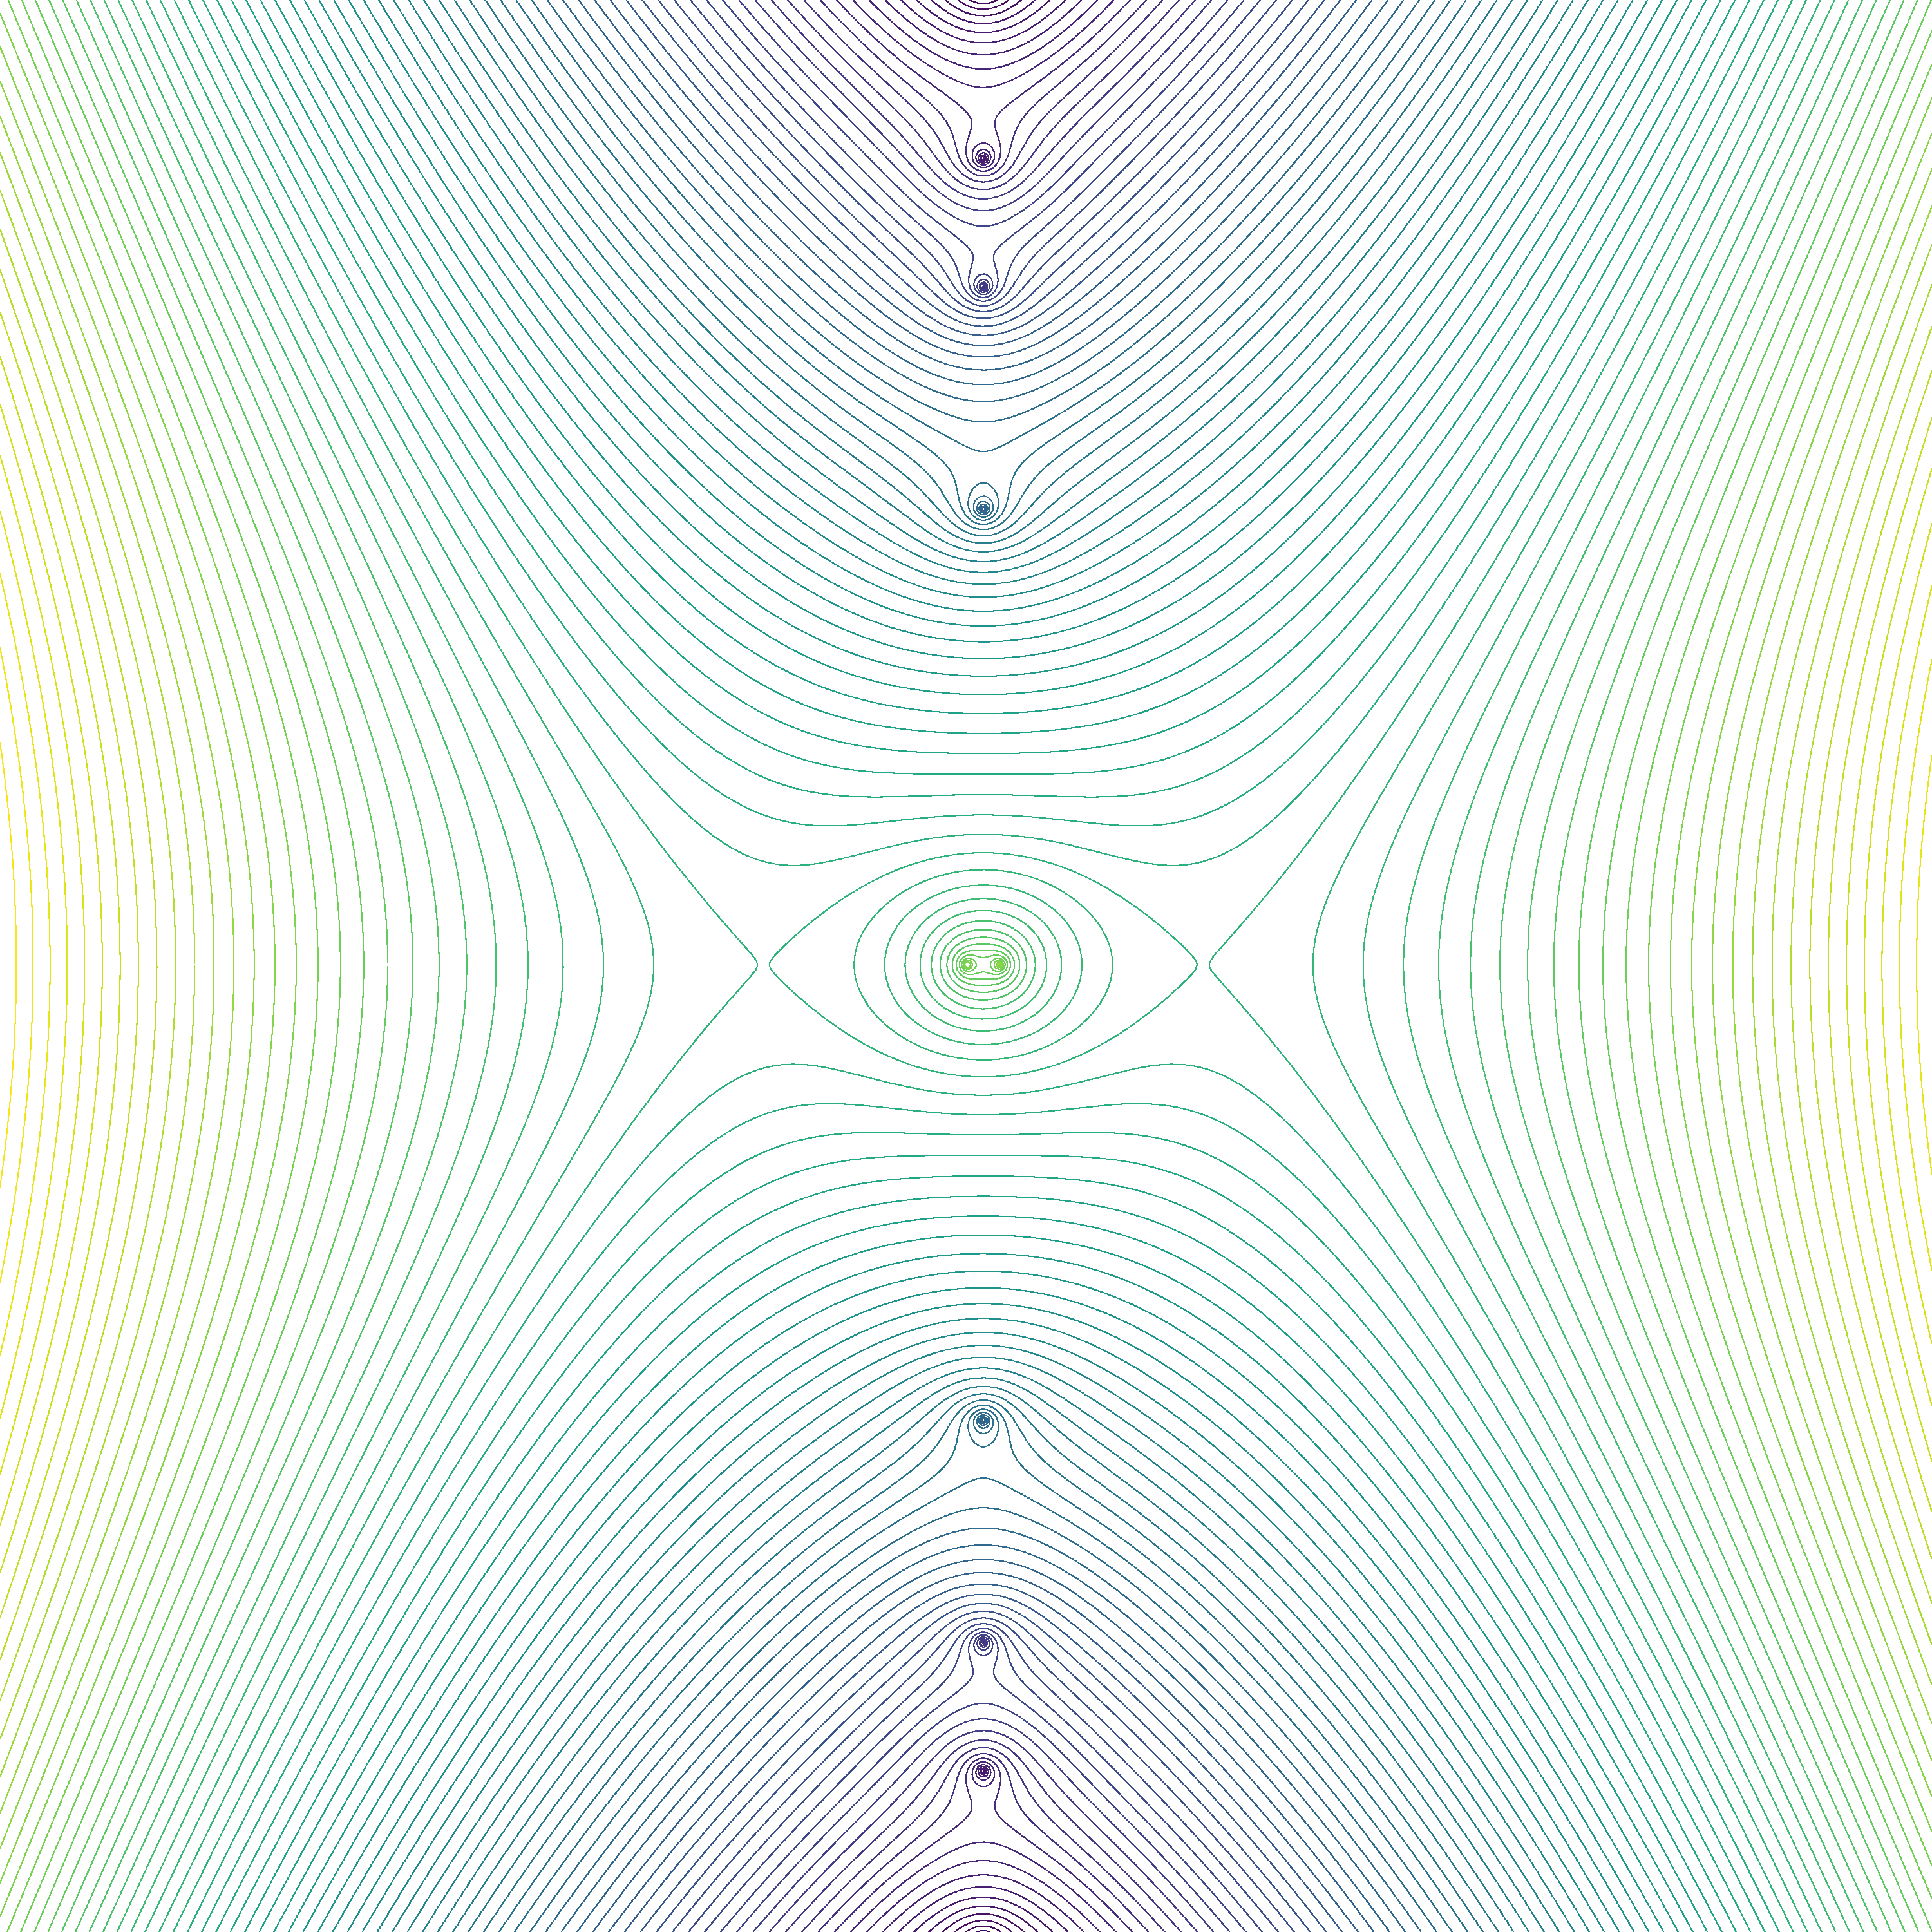
\includegraphics[width=0.55\textwidth]{figures/3030abs_contour_xi.pdf}};}
        \begin{scope}[x={(image.south east)},y={(image.north west)}]
            %\draw[help lines,xstep=.1,ystep=.1] (0,0) grid (1,1);
            \foreach \y in {-20,-10,...,20} {
                \node [anchor=east] at (0,\y/60+0.5) {$\y$}; 
                \draw (0,\y/60+0.5) -- (-1mm,\y/60+0.5);
                }
            \foreach \x in {-20,-10,0,1,10,20} { 
                \node [anchor=north] at (\x/56+0.5,0) {$\x$}; 
                \draw (\x/60+0.5,0) -- (\x/60+0.5,-1mm);
                }
            \node[rotate=90] (ylabel) at (-.12,0.5) {$\operatorname{\Im s}$};
            \node (xlabel) at (0.5,-.115) {$\operatorname{\Re s}$};
            \draw[very thin] (0,0) rectangle (1,1);
        \end{scope}
    \end{tikzpicture}%
    \vspace*{-13pt}
    \caption{\only<1>{Imaginärteil}\only<2>{Realteil}\only<3>{Betrag} der $\xi$-Funktion}
    \end{figure}
\end{frame}
\begin{frame}
    \frametitle{Nullstellenverteilung der $\xi$-Funktion}
    \begin{lemma}
        \[\xi(s) = 0\implies 0 \leq \Re s \leq 1\]
    \end{lemma}
    \begin{proof}
        Aufgrund der Eulerproduktdarstellung gilt
        \begin{itemize}[<+->]
            \item $0 \neq \zeta(s) = \frac{\pi^{s/2}}{\Gamma(s/2)}\xi(s) \quad \forall \Re s > 1$
            \item $\implies \xi(s) \neq 0 \Leftrightarrow \xi(1-s) \neq 0\quad \forall \Re s > 1$
            \item $\implies \xi(s) \neq 0 \quad \forall \Re s < 0$
        \end{itemize}
    \end{proof}
\end{frame}
\begin{frame}
    \begin{figure}%
        \begin{tikzpicture}
        \node[anchor=south west,inner sep=0] (image) at (0,0) {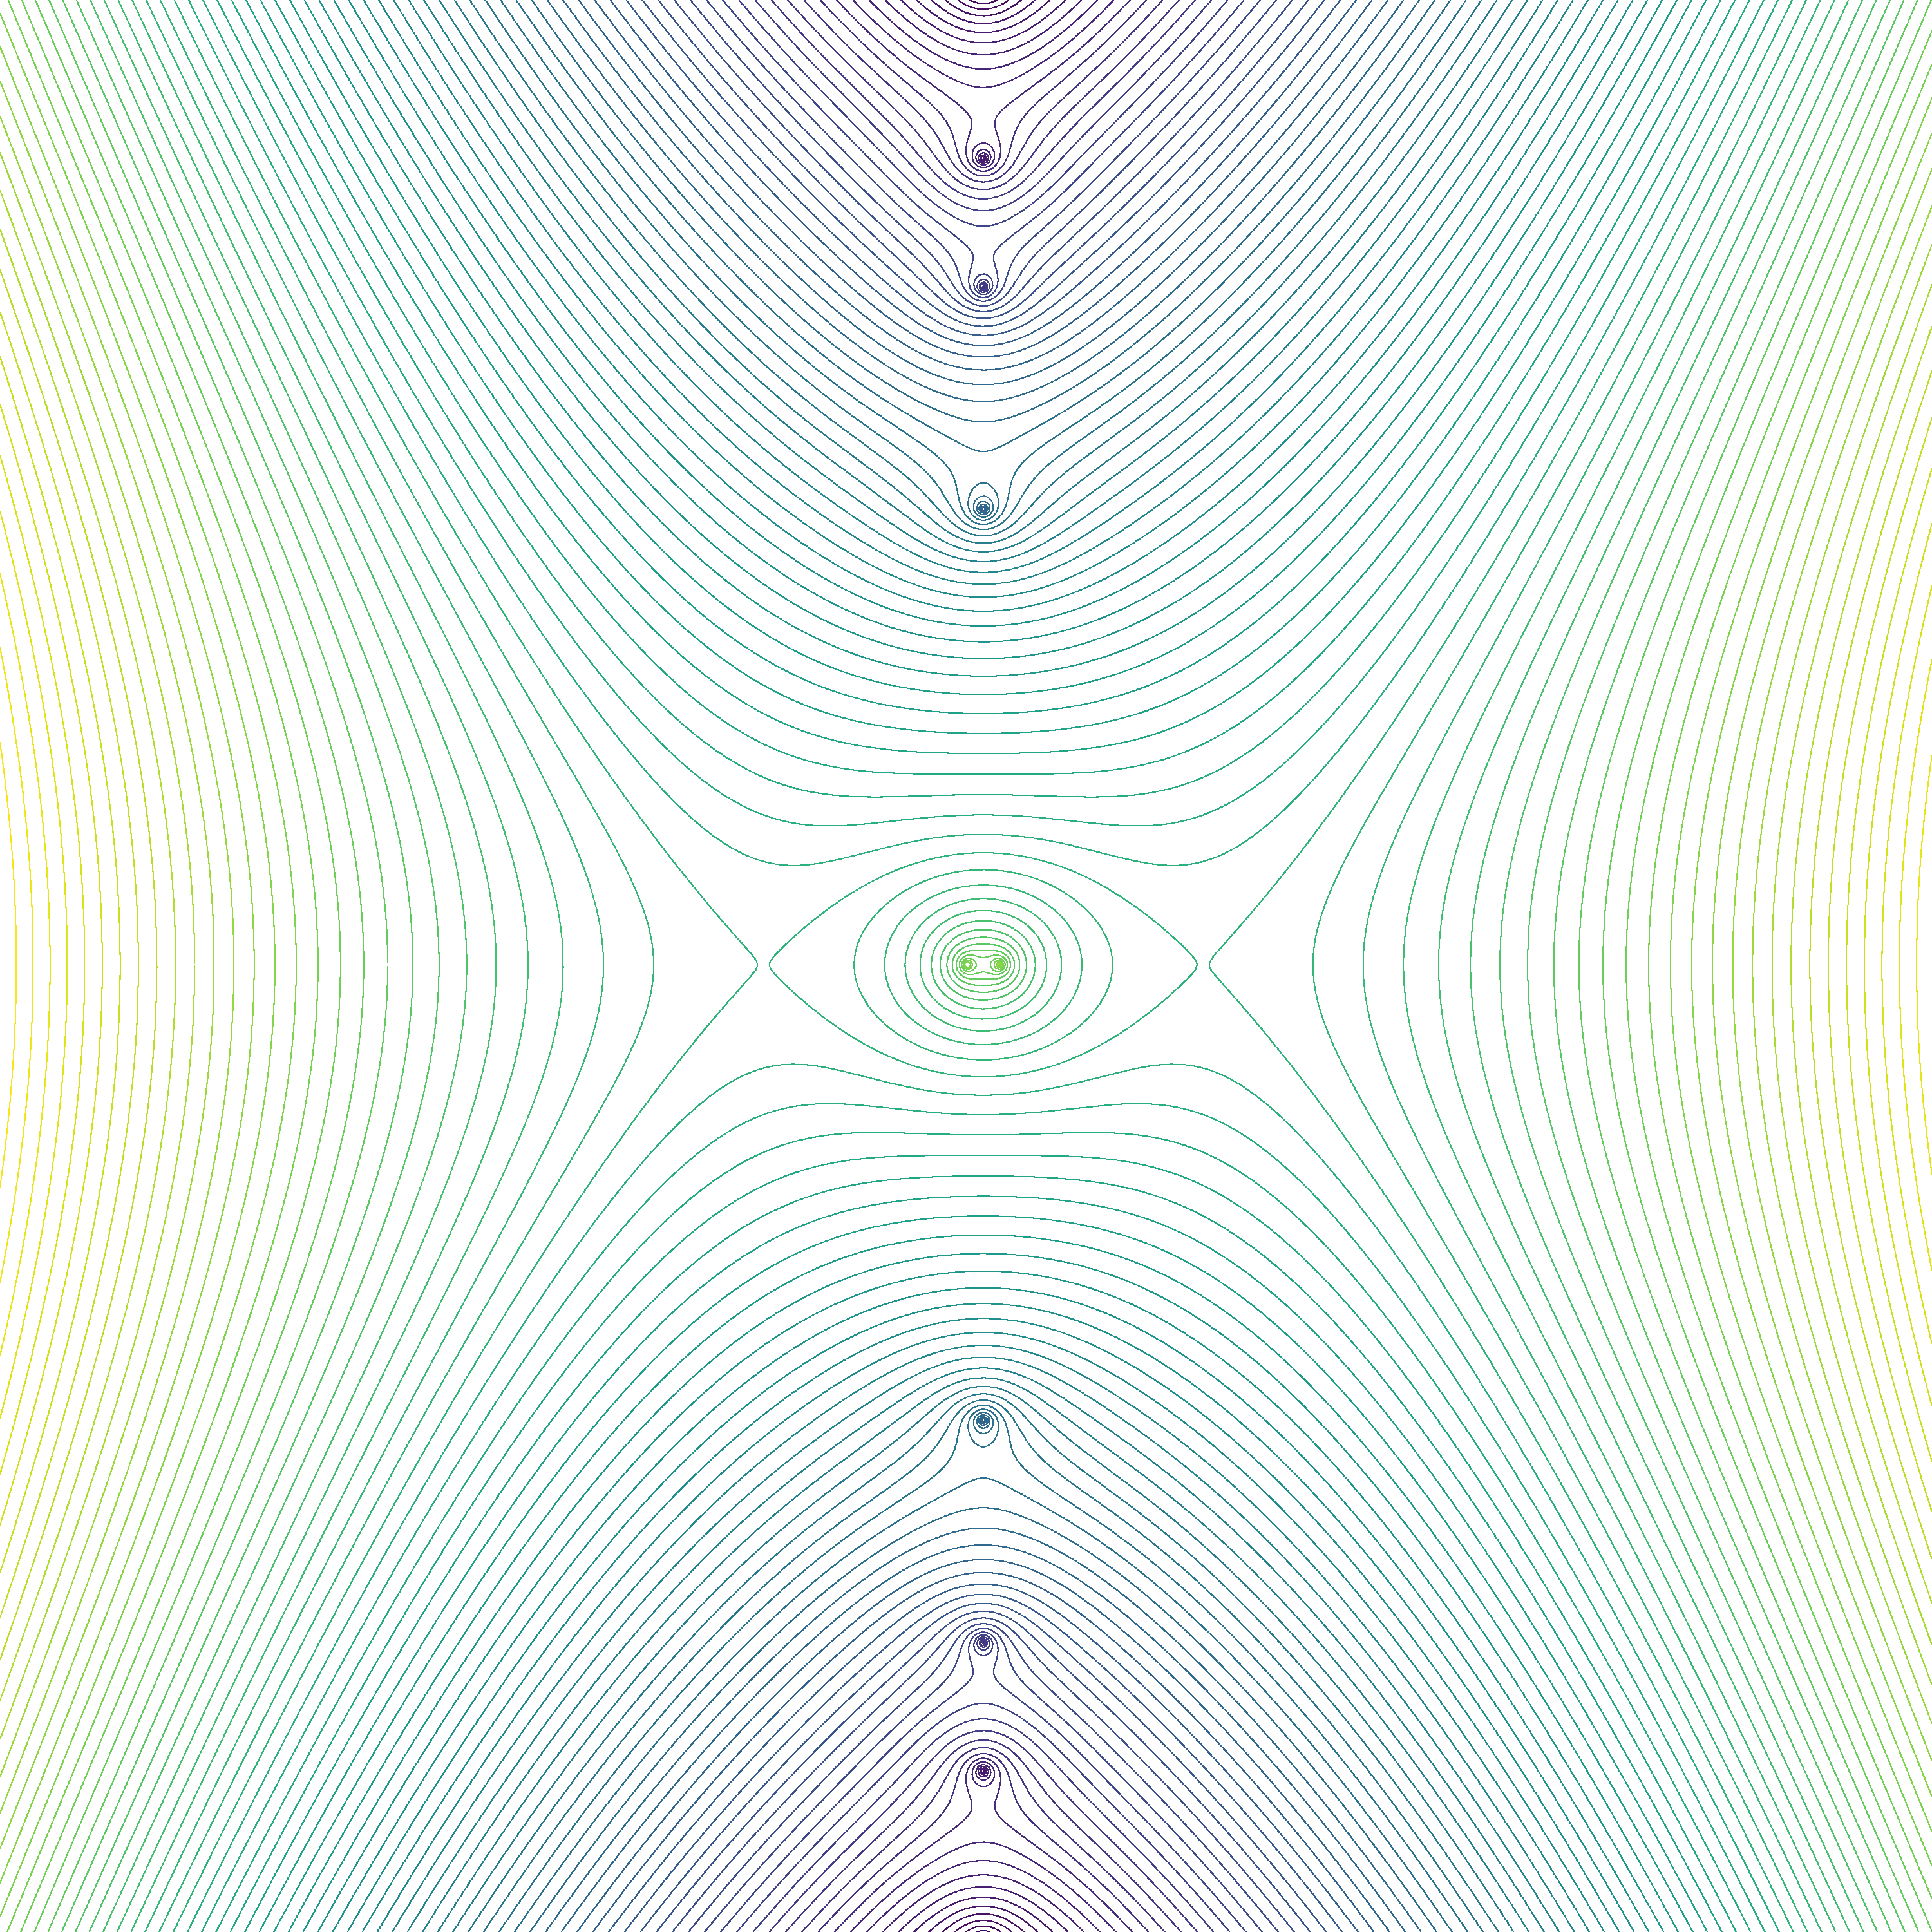
\includegraphics[width=0.55\textwidth]{figures/3030abs_contour_xi.pdf}};
        \begin{scope}[x={(image.south east)},y={(image.north west)}]
            %\draw[help lines,xstep=.1,ystep=.1] (0,0) grid (1,1);
            \foreach \y in {-20,-10,...,20} {
                \node [anchor=east] at (0,\y/60+0.5) {$\y$}; 
                \draw (0,\y/60+0.5) -- (-1mm,\y/60+0.5);
                }
            \foreach \x in {-20,-10,0,1,10,20} { 
                \node [anchor=north] at (\x/56+0.5,0) {$\x$}; 
                \draw (\x/60+0.5,0) -- (\x/60+0.5,-1mm);
                }
            \node[rotate=90] (ylabel) at (-.12,0.5) {$\operatorname{\Im s}$};
            \node (xlabel) at (0.5,-.115) {$\operatorname{\Re s}$};
            \draw[very thin] (0,0) rectangle (1,1);
            \only<2>{\fill[color=white, opacity=0.8] (0.52,0) rectangle (1,1);
            \fill[color=white, opacity=0.8] (0,0) rectangle (0.5,1);}
        \end{scope}
    \end{tikzpicture}%
    \vspace*{-13pt}
    \caption{Betrag der $\xi$-Funktion}
    \end{figure}
\end{frame}
\begin{frame}
    \frametitle{Nullstellenverteilung der $\zeta$-Funktion}
    \[
        \zeta(s) = \frac{\pi^{s/2}}{\Gamma(s/2)}\xi(s)  
    \]
    \begin{itemize}
        \item<2-> $\xi(s) = 0$ nur für $0 \leq \Re s \leq 1$.
        \item<3-> Genau für die Polstellen von $\Gamma(s/2)$ gilt $\frac{\pi^{2/s}}{\Gamma(s/2)} = 0$.
        \item<4-> $\implies \frac{\pi^{2/s}}{\Gamma(s/2)} = 0\qquad \forall s \in \{0,-2, -4, \dots\}$.
    \end{itemize}
    \visible<5->{
        \begin{block}{Folgerung.}
            $\zeta$ besitzt die \glqq trivialen Nullstellen\grqq\ bei $s = -2n,\; n\in \N$ und die Nullstellen von $\xi$, die allesamt im \glqq kritischen Streifen\grqq\  $0\leq \Re s \leq 1$ liegen.
        \end{block}
    }
\end{frame}
\begin{frame}[label=current]%
    \begin{figure}%
        \begin{tikzpicture}
        \node[anchor=south west,inner sep=0] (image) at (0,0) {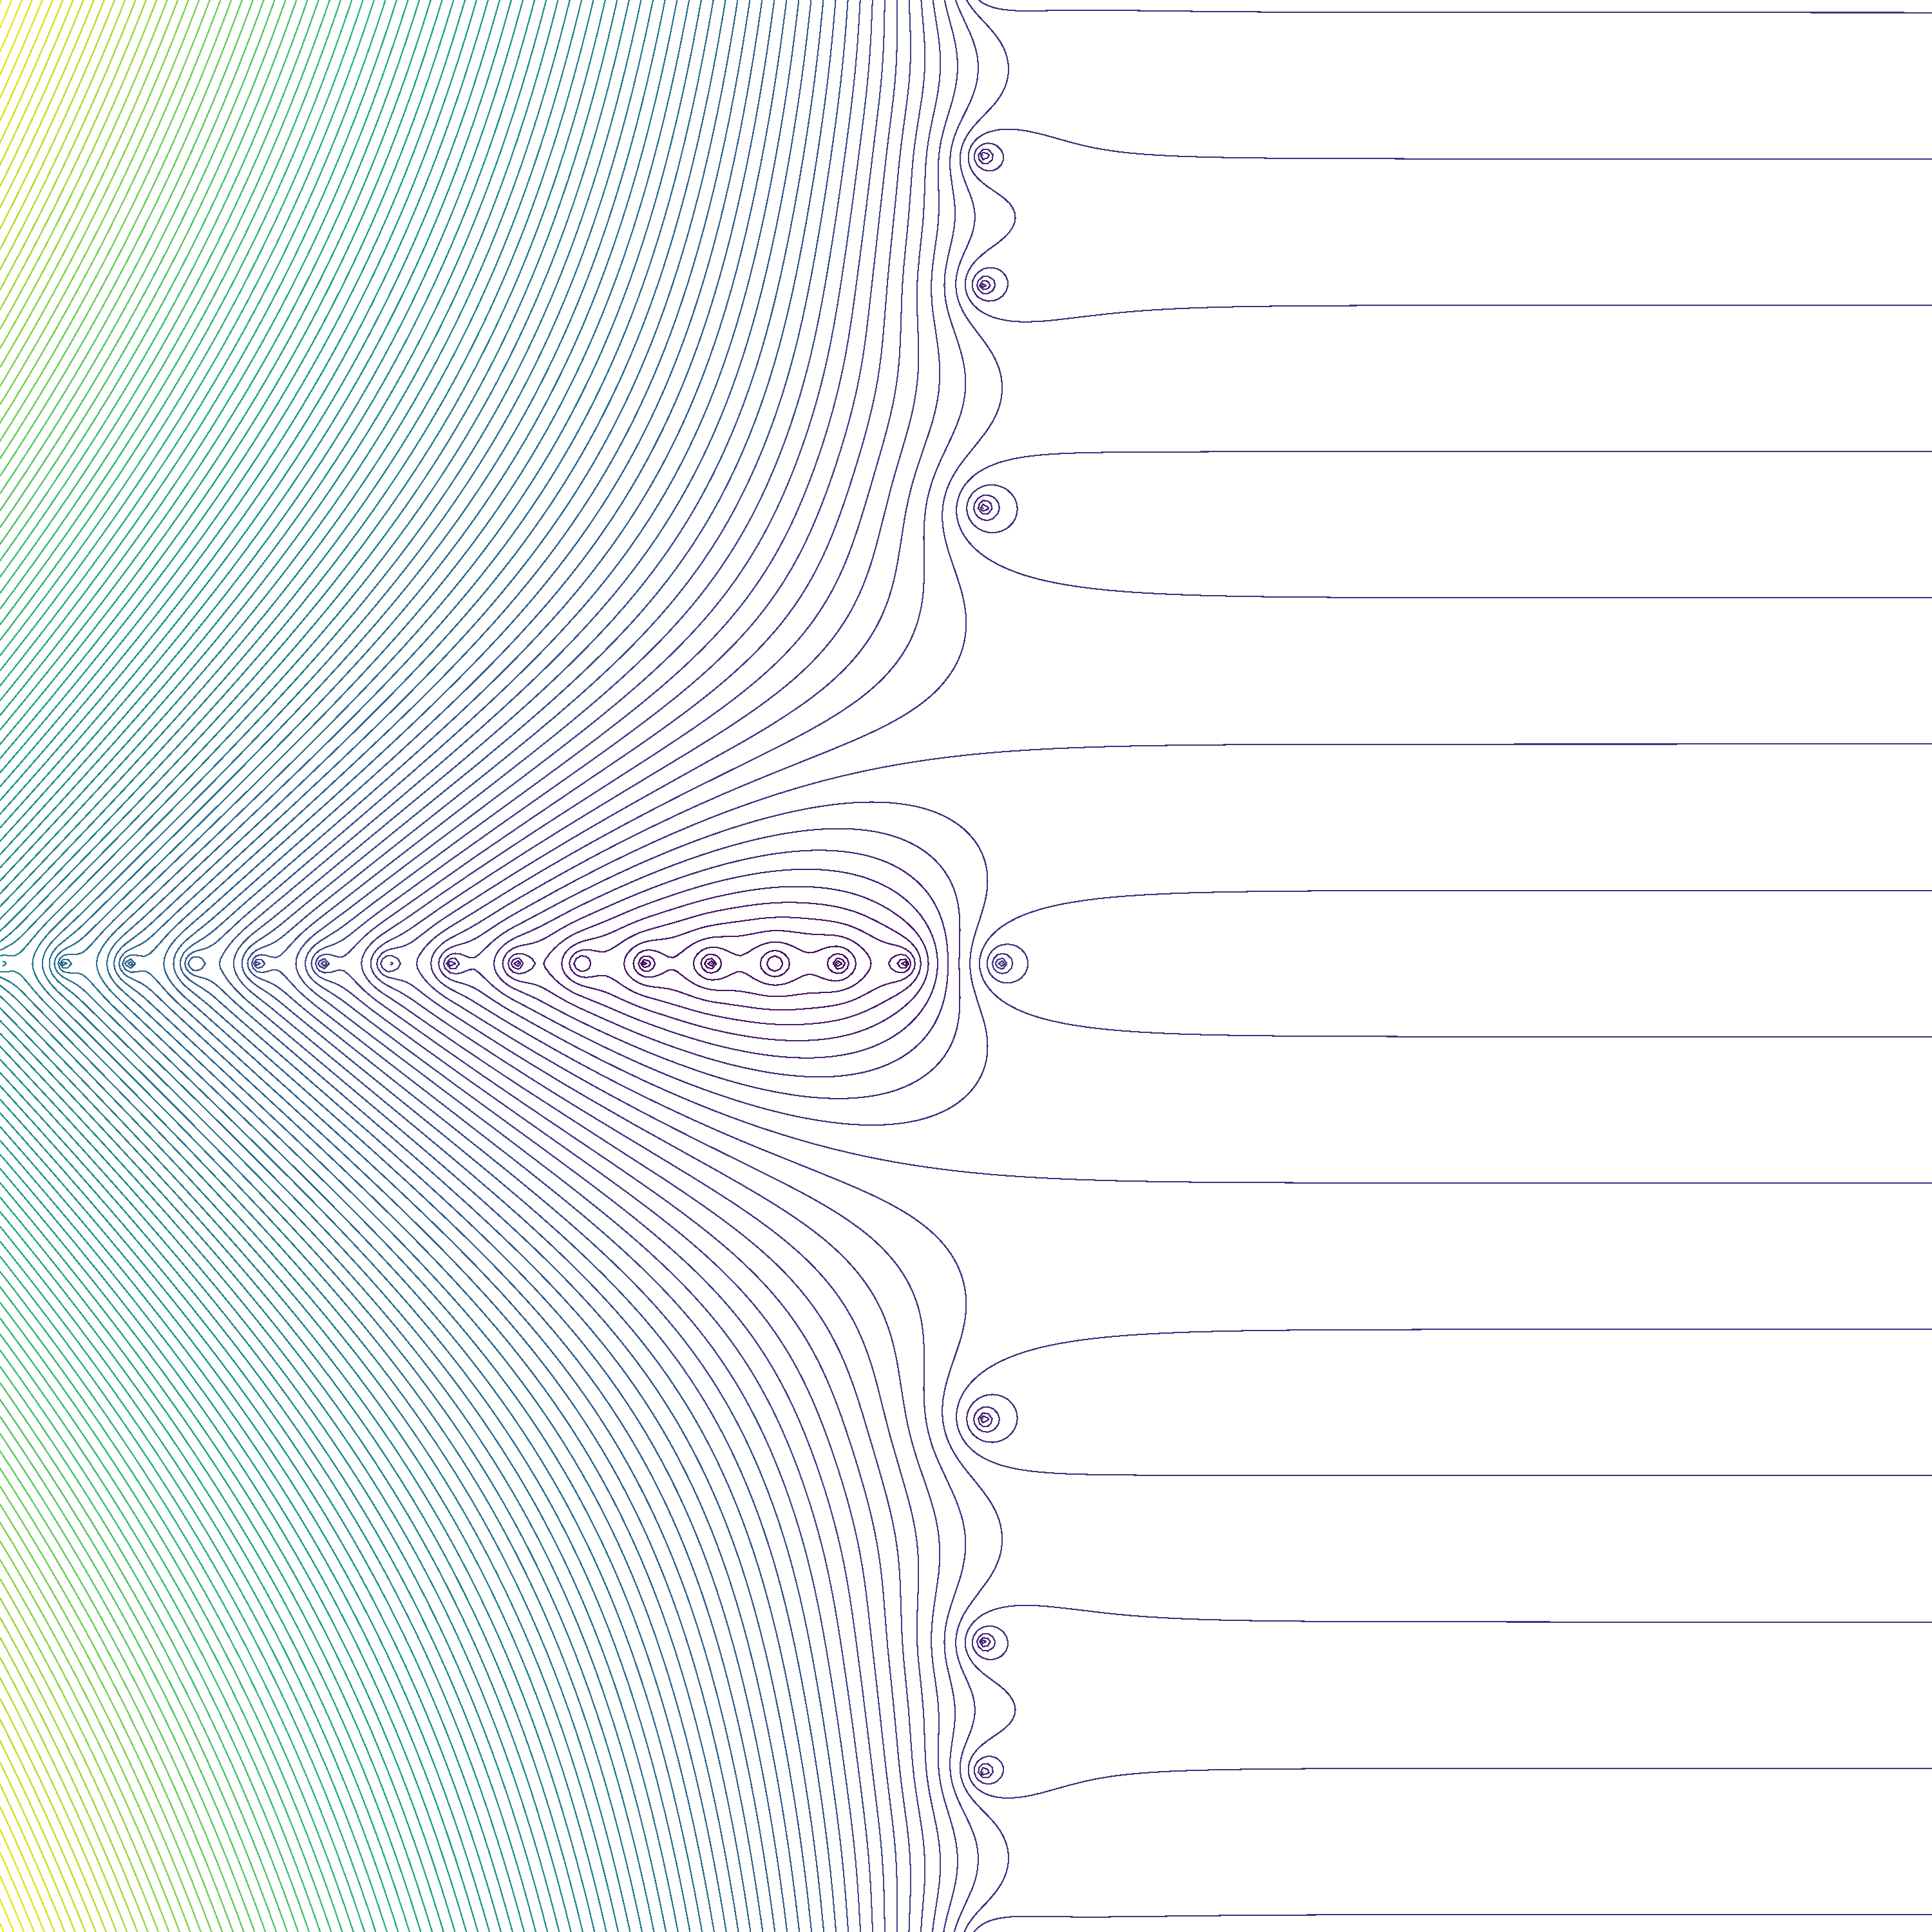
\includegraphics[width=0.55\textwidth]{figures/3030abs_contour_py.pdf}};
        \begin{scope}[x={(image.south east)},y={(image.north west)}]
            %\draw[help lines,xstep=.1,ystep=.1] (0,0) grid (1,1);
            \foreach \y in {-20,-10,...,20} {
                \node [anchor=east] at (0,\y/60+0.5) {$\y$}; 
                \draw (0,\y/60+0.5) -- (-1mm,\y/60+0.5);
                }
            \foreach \x in {-20,-10,0,1,10,20} { 
                \node [anchor=north] at (\x/56+0.5,0) {$\x$}; 
                \draw (\x/60+0.5,0) -- (\x/60+0.5,-1mm);
                }
            \node[rotate=90] (ylabel) at (-.12,0.5) {$\operatorname{\Im s}$};
            \node (xlabel) at (0.5,-.115) {$\operatorname{\Re s}$};
            \draw[very thin] (0,0) rectangle (1,1);
            \fill[color=white, opacity=0.8] (0.52,0) rectangle (1,1);
            \only<2->{\fill[color=white, opacity=0.8] (0,0) rectangle (0.5,1);}
        \end{scope}
    \end{tikzpicture}%
    \vspace*{-13pt}
    \caption{Betrag der $\zeta$-Funktion}
    \end{figure}
\end{frame}
\begin{frame}
    \begin{hypothesis}[Riemannsche Hypothese]
        Abgesehen von den \glqq trivialen\grqq\ Nullstellen bei $s = -2n,\; n\in \N$ haben alle Nullstellen Realteil $\frac{1}{2}$.
    \end{hypothesis}
    \only<1>{
    \begin{figure}
        \begin{tikzpicture}
            \node[anchor=south west,inner sep=0] (image) at (0,0) {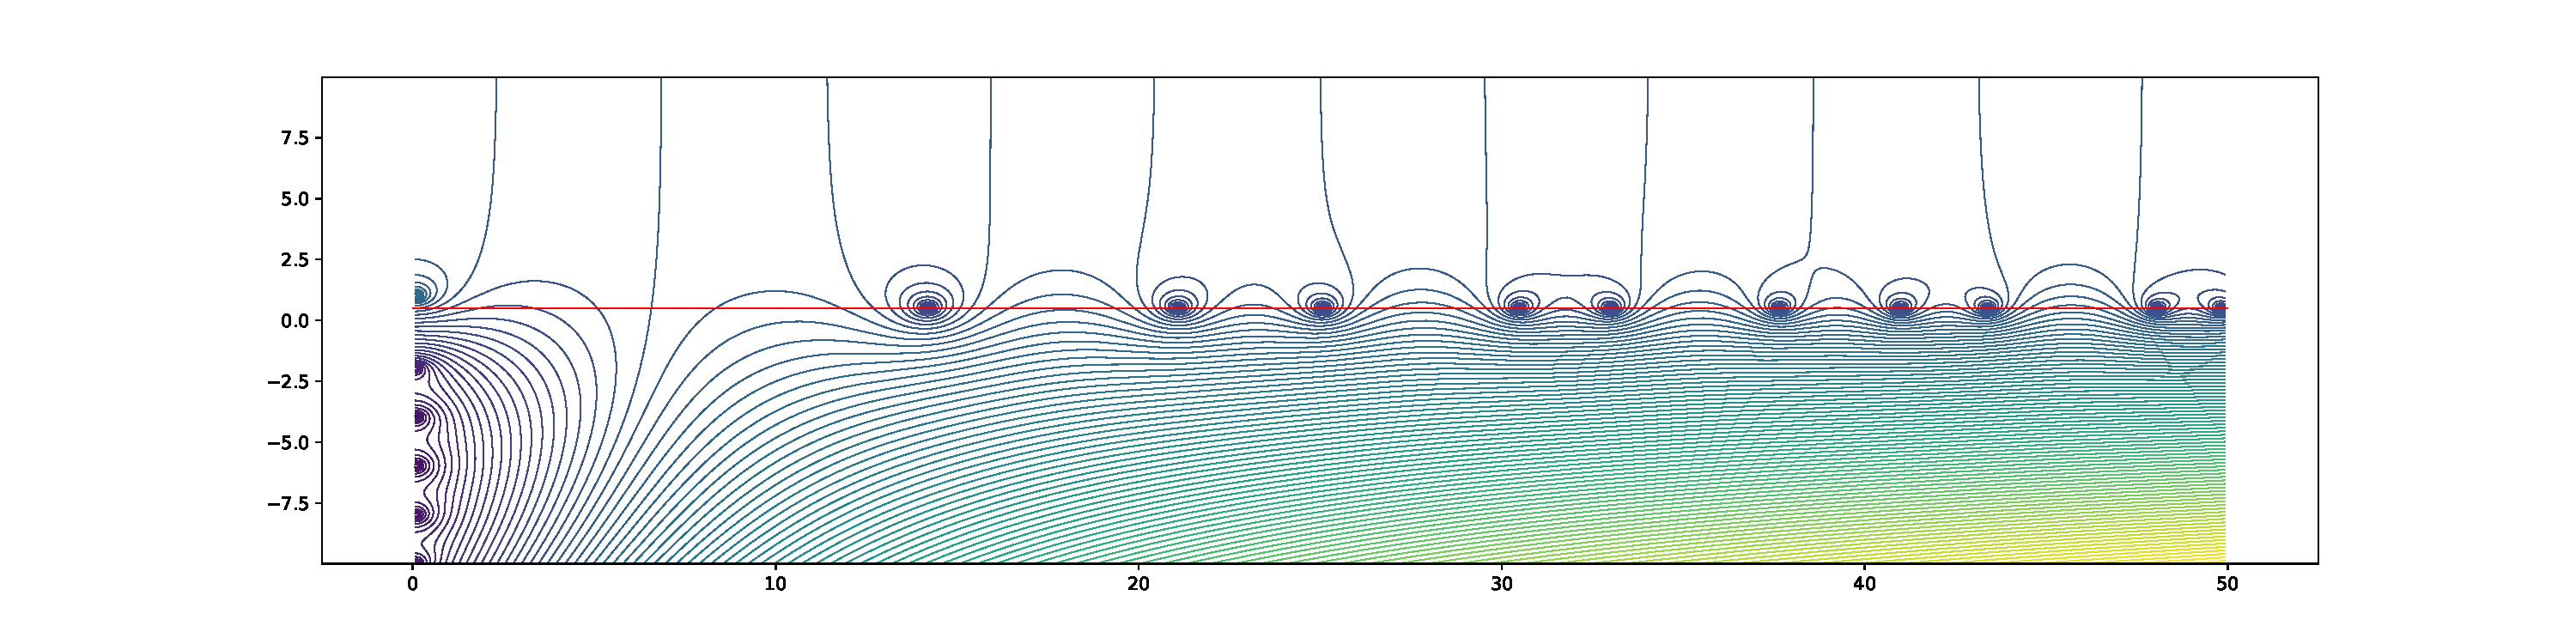
\includegraphics[width=0.8\textwidth, trim=231 46 195 44, clip]{figures/jupyter_zeros.pdf}};
            \begin{scope}[x={(image.south east)},y={(image.north west)}]
                %\draw[help lines,xstep=.1,ystep=.1] (0,0) grid (1,1);
                \foreach \y in {-10,-5,...,10} { 
                    \node [anchor=east] at (0,\y/20+0.5) {$\y$}; 
                    \draw (0,\y/20+0.5) -- (-1mm,\y/20+0.5);
                    }
                \foreach \x in {0,10,...,50} { 
                    \node [anchor=north] at (\x/50,0) {$\x$}; 
                    \draw (\x/50,0) -- (\x/50,-1mm);
                    }
                \node (ylabel) at (-.12,0.5) {$\operatorname{\Re s}$};
                \node (xlabel) at (0.5,-.25) {$\operatorname{\Im s}$};
                \draw[very thin] (0,0) rectangle (1,1);
            \end{scope}
        \end{tikzpicture}
        \caption{Absolutbetrag der $\zeta$-Funktion bei $\Re s = \frac{1}{2}$ von $\Im s = 0$ bis $\Im s = 50$}
    \end{figure}
    }
    \only<2>{
        \begin{center}
            \sagestr{output}
        \end{center}
    }
\end{frame}
\begin{frame}
    \frametitle{Konsequenzen der Riemannschen Hypothese}

    \begin{definition}
        \[
            \mu(n) = \begin{cases}
                (-1)^k & n \text{ ist quadratfrei und hat $k$ Primfaktoren}\\
                0 & \text{sonst}
            \end{cases}  
        \]
    \end{definition}
    \begin{lemma}
        Es gilt \[
            \frac{1}{\zeta(s)} = \sum_{n = 1}^{\infty} \frac{\mu(n)}{n^s}  
        \] für $\Re s > 1$ mit
    \end{lemma}
\end{frame}
\begin{frame}
    \frametitle{Konsequenzen der Riemannschen Hypothese}
    \begin{proof}\vspace*{-0.5cm}
        \[
            \frac{1}{\zeta(s)} = \prod_{k=1}^\infty \left(1 - \frac{1}{p_k^s}\right) = \left(1 - \frac{1}{2^s}\right)\left(1 - \frac{1}{3^s}\right) \dots = \sum_{n = 1}^{\infty} \frac{\mu(n)}{n^s} 
        \]
    \end{proof}
    \begin{theorem}
        Die Gleichung \[
            \frac{1}{\zeta(s)} = \sum_{n = 1}^{\infty} \frac{\mu(n)}{n^s}
        \] für $\Re s > \frac{1}{2}$ ist äquivalent zur Riemannschen Hypothese.
    \end{theorem}
\end{frame}
\begin{frame}
    \frametitle{Literarurverzeichnis}

    \begin{thebibliography}{Freitag und Busam, 2000}
        \bibitem[Neukirch, 1992]{Neukirch1992}
            J.~Neukirch.
            \newblock {\em Algebraische Zahlentheorie}.
            \newblock Springer-Verlag Berlin Heidelberg, 1992.
        \bibitem[Freitag und Busam, 2000]{FuB2000}
            E.~Freitag., R.~Busam
            \newblock {\em Funktionentheorie 1}.
            \newblock Springer-Verlag Berlin Heidelberg, 2000.
    \end{thebibliography}

\end{frame}
\appendix
% This file was created by tikzplotlib v0.9.4.
\begin{tikzpicture}

\definecolor{color0}{rgb}{0.12156862745098,0.466666666666667,0.705882352941177}

\begin{axis}[
legend cell align={left},
legend style={fill opacity=0.8, draw opacity=1, text opacity=1, at={(0.03,0.97)}, anchor=north west, draw=white!80!black},
tick align=outside,
tick pos=left,
x grid style={white!69.0196078431373!black},
xmin=0.1, xmax=19.9,
xtick style={color=black},
y grid style={white!69.0196078431373!black},
ymin=-0.35, ymax=7.35,
ytick style={color=black}
]
\addplot [semithick, color0, const plot mark right]
table {%
1 0
2 0
3 1
4 2
5 2
6 3
7 3
8 4
9 4
10 4
11 4
12 5
13 5
14 6
15 6
16 6
17 6
18 7
19 7
};
\addlegendentry{$\pi(x)$}
\end{axis}

\end{tikzpicture}

\begin{frame}
    \frametitle{Konsequenzen der Riemannschen Hypothese}
    \only<1>{
        \begin{lemma}
            \[
                \sigma(n) = \sum_{d | n} d < e^\gamma n \log \log n + \frac{0.6483\ n}{\log \log n}
            \]
        \end{lemma}
        \begin{theorem}[Robin, 1984]
            Die Abschätzung \[
                \sigma(n) < e^\gamma n \log \log n 
                    \]
            ist äquivalent zur Riemannschen Hypothese.
        \end{theorem}
    }
    \only<2>{
        \begin{figure}
            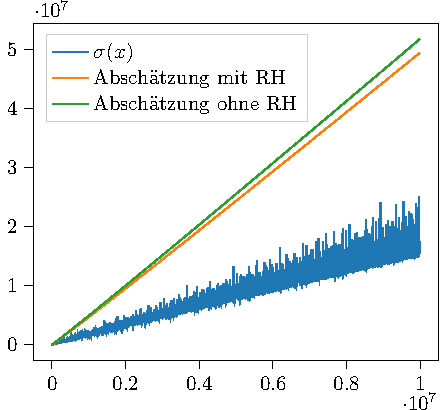
\includegraphics[scale=0.9]{figures/robins_inequality_plot.pdf}
        \end{figure}
    }
\end{frame}
\end{document}